% Options for packages loaded elsewhere
\PassOptionsToPackage{unicode}{hyperref}
\PassOptionsToPackage{hyphens}{url}
\documentclass[
]{article}
\usepackage{xcolor}
\usepackage[margin=1in]{geometry}
\usepackage{amsmath,amssymb}
\setcounter{secnumdepth}{5}
\usepackage{iftex}
\ifPDFTeX
  \usepackage[T1]{fontenc}
  \usepackage[utf8]{inputenc}
  \usepackage{textcomp} % provide euro and other symbols
\else % if luatex or xetex
  \usepackage{unicode-math} % this also loads fontspec
  \defaultfontfeatures{Scale=MatchLowercase}
  \defaultfontfeatures[\rmfamily]{Ligatures=TeX,Scale=1}
\fi
\usepackage{lmodern}
\ifPDFTeX\else
  % xetex/luatex font selection
\fi
% Use upquote if available, for straight quotes in verbatim environments
\IfFileExists{upquote.sty}{\usepackage{upquote}}{}
\IfFileExists{microtype.sty}{% use microtype if available
  \usepackage[]{microtype}
  \UseMicrotypeSet[protrusion]{basicmath} % disable protrusion for tt fonts
}{}
\makeatletter
\@ifundefined{KOMAClassName}{% if non-KOMA class
  \IfFileExists{parskip.sty}{%
    \usepackage{parskip}
  }{% else
    \setlength{\parindent}{0pt}
    \setlength{\parskip}{6pt plus 2pt minus 1pt}}
}{% if KOMA class
  \KOMAoptions{parskip=half}}
\makeatother
\usepackage{longtable,booktabs,array}
\newcounter{none} % for unnumbered tables
\usepackage{calc} % for calculating minipage widths
% Correct order of tables after \paragraph or \subparagraph
\usepackage{etoolbox}
\makeatletter
\patchcmd\longtable{\par}{\if@noskipsec\mbox{}\fi\par}{}{}
\makeatother
% Allow footnotes in longtable head/foot
\IfFileExists{footnotehyper.sty}{\usepackage{footnotehyper}}{\usepackage{footnote}}
\makesavenoteenv{longtable}
\usepackage{graphicx}
\makeatletter
\newsavebox\pandoc@box
\newcommand*\pandocbounded[1]{% scales image to fit in text height/width
  \sbox\pandoc@box{#1}%
  \Gscale@div\@tempa{\textheight}{\dimexpr\ht\pandoc@box+\dp\pandoc@box\relax}%
  \Gscale@div\@tempb{\linewidth}{\wd\pandoc@box}%
  \ifdim\@tempb\p@<\@tempa\p@\let\@tempa\@tempb\fi% select the smaller of both
  \ifdim\@tempa\p@<\p@\scalebox{\@tempa}{\usebox\pandoc@box}%
  \else\usebox{\pandoc@box}%
  \fi%
}
% Set default figure placement to htbp
\def\fps@figure{htbp}
\makeatother
\setlength{\emergencystretch}{3em} % prevent overfull lines
\providecommand{\tightlist}{%
  \setlength{\itemsep}{0pt}\setlength{\parskip}{0pt}}
\usepackage[]{natbib}
\bibliographystyle{plainnat}
\usepackage{graphicx}
\usepackage{float}
\usepackage{booktabs}
\usepackage{longtable}
\usepackage{caption}
\usepackage{listings}
\usepackage{xcolor}
\usepackage{hyperref}
\usepackage{url}
\usepackage{etoolbox}
\usepackage{natbib}

\renewcommand{\refname}{}
\renewcommand{\bibname}{}

% --- Title handling ---
\title{$title$}
\author{$author$}
\date{$date$}

\AtBeginDocument{
  \maketitle
  %\tableofcontents
  \clearpage
}

% --- allow alt= ---
\makeatletter
\define@key{Gin}{alt}{}
\makeatother

% --- scale figures ---
\makeatletter
\def\maxwidth{\ifdim\Gin@nat@width>\linewidth\linewidth\else\Gin@nat@width\fi}
\makeatother

\setkeys{Gin}{width=\maxwidth,height=0.8\textheight,keepaspectratio}

% --- syntax highlighting (arXiv-safe) ---
\lstdefinelanguage{Python}{
  keywords={def, return, if, else, elif, for, while, import, from, as, class, try, except, raise, with, lambda, yield, True, False, None},
  keywordstyle=\color{blue}\bfseries,
  comment=[l]{\#},
  commentstyle=\color{gray}\itshape,
  stringstyle=\color{red},
  morestring=[b]',
  morestring=[b]",
}

\lstset{
  language=Python,
  basicstyle=\ttfamily\small,
  keywordstyle=\color{blue}\bfseries,
  commentstyle=\color{gray}\itshape,
  stringstyle=\color{red},
  breaklines=true,
  frame=single,
  showstringspaces=false,
  columns=fullflexible,
  keepspaces=true
}

% --- new page per section ---
%\pretocmd{\section}{\clearpage}{}{}
\makeatletter
\pretocmd{\section}{%
  \ifnum\pdfstrcmp{\@currentlabelname}{References}=0
    % do nothing
  \else
    \clearpage
  \fi
}{}{}
\makeatother

% --- nicer captions ---
\captionsetup{
  font=small,
  labelfont=bf
}

% --- FIX bold-text bug ---
\normalfont
\renewcommand{\familydefault}{\rmdefault}
\usepackage{bookmark}
\IfFileExists{xurl.sty}{\usepackage{xurl}}{} % add URL line breaks if available
\urlstyle{same}
\hypersetup{
  hidelinks,
  pdfcreator={LaTeX via pandoc}}

\title{Boolean Network Modeling in Systems Biology: A Hands-On Tutorial with BoolForge}
\author{Claus Kadelka}
\date{March 31, 2026}

\begin{document}
\maketitle

{
\setcounter{tocdepth}{3}
\tableofcontents
}
\section*{Abstract}\label{abstract}
\addcontentsline{toc}{section}{Abstract}

Boolean networks are a widely used modeling framework for studying
complex dynamical systems in systems biology, including gene regulatory
and signaling networks. Despite their conceptual simplicity, practical
challenges -- such as constructing biologically meaningful models,
analyzing dynamical behavior, and generating appropriate null models --
often limit their accessibility, reproducibility, and systematic use.

We present a comprehensive, hands-on tutorial to Boolean network
modeling and analysis, accompanied by the Python package BoolForge. This
tutorial is designed for researchers and students with diverse
backgrounds and provides a step-by-step introduction ranging from basic
concepts to advanced topics. Covered topics include Boolean functions
and their representations, canalization, random function generation
under structural constraints, construction of Boolean networks and
wiring diagrams, synchronous and asynchronous dynamics, attractor and
basin analysis, robustness and coherence measures, and the generation of
controlled null models for hypothesis testing.

Emphasis is placed on reproducible computational workflows and the
systematic investigation of structure--dynamics relationships. Through a
series of progressively developed examples and executable code snippets,
readers learn how to construct, analyze, and interpret Boolean network
models, as well as how to generate ensembles of randomized networks that
preserve key structural features such as degree distribution, bias, and
canalizing depth. Code and tutorials are openly available at
\url{https://github.com/ckadelka/BoolForge}.

This tutorial serves both as a practical introduction for new users and
as a reference for advanced researchers seeking to apply Boolean network
methods in systems biology. By integrating theory, algorithms, and
software implementation, it aims to facilitate the adoption of rigorous
and reproducible modeling practices in the study of complex biological
systems.

\section*{Preface}\label{preface}
\addcontentsline{toc}{section}{Preface}

This tutorial is designed as a hands-on, computational introduction to
Boolean network modeling using BoolForge.

Rather than focusing purely on theory, we emphasize executable workflows
and reproducible experiments. The goal is to enable readers to explore
structure-dynamics relationships directly through code.

To illustrate the type of analyses enabled by BoolForge, we begin with a
simple example reproducing Derrida's classical phase transition (see
\citet{derrida1986random}) in a few lines of BoolForge code.

\begin{lstlisting}
import boolforge as bf
import matplotlib.pyplot as plt

N = 100          # network size
ks = range(1,5)  # constant in-degree
n_networks = 50  # ensemble size
p = 0.5          # bias p: probability of ones in truth table

derrida_values = []
for k in ks:
    derrida_values.append([])
    for _ in range(n_networks):
        bn = bf.random_network(N, k, bias = p, allow_degenerate_functions=True)
        derrida_values[-1].append( bn.get_derrida_value(exact=True) )

plt.boxplot(derrida_values, positions=list(ks))
plt.axhline(1, linestyle="--", color="gray", label="critical value")
plt.plot(ks, [2*k*p*(1-p) for k in ks], "o-", label=r"$2kp(1-p)$ (annealed theory)")
plt.xlabel("Constant in-degree k")
plt.ylabel("Derrida value")
plt.legend(frameon=False);
\end{lstlisting}

\pandocbounded{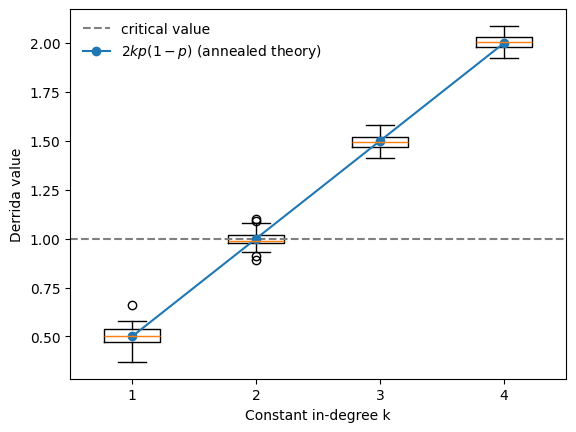
\includegraphics[keepaspectratio]{figures/tutorial00_preface_tex_fig0.png}}

The Derrida value measures the average number of nodes affected by a
single-bit random perturbation after one synchronous update of the
network.

\subsection*{Structure of the
tutorials}\label{structure-of-the-tutorials}
\addcontentsline{toc}{subsection}{Structure of the tutorials}

The tutorials gradually introduce the main concepts and tools provided
by BoolForge, moving from individual Boolean functions to full Boolean
network models and their dynamical analysis.

\begin{itemize}
\tightlist
\item
  \emph{Boolean functions:} representation and structural analysis
\item
  \emph{Canalization:} redundancy and robustness of regulatory rules
\item
  \emph{Random function generation:} sampling functions with prescribed
  properties
\item
  \emph{Boolean networks:} construction and wiring diagrams
\item
  \emph{Network dynamics:} attractors and state transition graphs
\item
  \emph{Stability and robustness:} sensitivity to perturbations
\item
  \emph{Random network ensembles:} statistical analysis of network
  dynamics
\item
  \emph{Biological models:} analysis of curated regulatory networks
\end{itemize}

Each tutorial contains executable code examples illustrating how these
ideas can be explored using BoolForge. Corresponding Jupyter notebook
(ipynb) files can be found at
\url{https://github.com/ckadelka/BoolForge/tree/main/tutorials}. Readers
are encouraged to run the code cells and modify the examples to explore
their own Boolean functions and networks.

\section*{Introduction}\label{introduction}
\addcontentsline{toc}{section}{Introduction}

Boolean networks have emerged as a central modeling framework for
studying complex dynamical systems in systems biology, including gene
regulatory, signaling, and cellular decision-making networks
\citep{kauffman1969metabolic}. In a Boolean network, each component is
represented by a binary variable, and its dynamics are governed by
logical update rules that capture regulatory interactions. Despite their
conceptual simplicity, Boolean networks are capable of reproducing rich
dynamical behavior such as multistability, oscillations, and robustness
to perturbations, making them a widely used tool for qualitative
modeling when detailed kinetic information is unavailable.

Over the past decades, Boolean network models have been successfully
applied to a broad range of biological systems, from cell cycle
regulation to developmental processes and disease-related signaling
pathways. At the same time, theoretical advances have deepened our
understanding of how structural properties---such as network topology,
regulatory logic, and canalization---shape dynamical behavior. In
particular, concepts such as attractors, basins of attraction,
robustness, and sensitivity have become standard tools for analyzing the
long-term behavior of these systems.

However, despite this progress, practical challenges remain.
Constructing biologically meaningful Boolean network models, analyzing
their dynamics, and interpreting results in a reproducible and
systematic way can be difficult, especially for researchers new to the
field. Moreover, many commonly used approaches rely on ad hoc
randomization or lack appropriate null models, making it challenging to
disentangle the effects of network structure from those of the update
rules. As a result, there is a growing need for tools and tutorials that
integrate theoretical concepts with practical, reproducible workflows.

This tutorial addresses these challenges by providing a comprehensive,
hands-on introduction to Boolean network modeling and analysis,
accompanied by the Python package BoolForge. The goal is to bridge the
gap between theory and practice by guiding the reader from fundamental
concepts to advanced applications, with an emphasis on reproducibility,
clarity, and methodological rigor.

We begin by introducing Boolean functions and their representations,
including truth tables and logical expressions, and discuss key
structural properties such as bias, essential variables, and
canalization. We then present methods for generating random Boolean
functions under structural constraints, including \(k\)-canalizing
functions and nested canalizing functions, which play a central role in
biological modeling. Building on these foundations, we introduce Boolean
networks and wiring diagrams, and demonstrate how to construct and
manipulate models programmatically.

A central focus of this tutorial is the analysis of network dynamics. We
cover both synchronous and asynchronous update schemes, and describe
methods for identifying attractors, computing basins of attraction, and
quantifying dynamical properties such as robustness, fragility, and
coherence. In addition, we emphasize the importance of ensemble-based
approaches and controlled null models, which allow systematic
investigation of how structural features---such as degree distribution,
bias, and canalizing depth---affect network behavior.

Throughout the tutorial, we provide executable code examples and
reproducible workflows that enable readers to directly apply the
presented methods to their own research questions. By integrating
theory, algorithms, and software implementation, this tutorial aims to
make Boolean network modeling more accessible, transparent, and
rigorous.

This document is intended for a broad audience, including students,
experimentalists, and computational researchers. Readers new to Boolean
networks will find a step-by-step introduction to the key concepts and
methods, while more experienced users may use this tutorial as a
reference for advanced topics such as constrained random function
generation and null model construction.

\subsection*{Positioning within the
literature}\label{positioning-within-the-literature}
\addcontentsline{toc}{subsection}{Positioning within the literature}

While numerous introductions to Boolean networks exist, they are often
fragmented across textbooks, review articles, and software-specific
documentation, and typically emphasize either theoretical aspects or
particular applications. In contrast, this tutorial provides a unified,
end-to-end treatment that integrates structural theory, dynamical
analysis, and reproducible computational workflows within a single
framework. A distinguishing feature is the systematic treatment of
constrained random function and network generation, including
canalization-controlled ensembles and null models that preserve key
structural properties. This enables rigorous investigation of
structure--dynamics relationships beyond traditional random network
paradigms. By combining these methodological advances with practical
implementation in BoolForge, this work is positioned not merely as an
introduction, but as a comprehensive reference for modern Boolean
network analysis in systems biology.

\textbf{Citation note}. If you use BoolForge in your research, please
cite the accompanying software paper \citep{kadelka2025boolforge}. If
this tutorial contributed to your modeling, analysis, or interpretation,
please cite this work.

\section{Working with Boolean
Functions}\label{working-with-boolean-functions}

Boolean functions are the building blocks of Boolean network models used
to represent gene regulatory networks, signaling pathways, and other
biological control systems. Understanding how to create and analyze
individual Boolean functions is essential before studying network-level
dynamics.

In this tutorial, we explore the \texttt{BooleanFunction} class --- the
foundation of BoolForge. Boolean functions form the regulatory rules in
Boolean network models of gene regulation, so understanding their
structure is essential before studying networks.

\subsection{What you will learn}\label{what-you-will-learn}

In this tutorial you will:

\begin{itemize}
\tightlist
\item
  create Boolean functions from truth tables and from textual
  expressions,
\item
  inspect core attributes such as degree, variable names, and stored
  properties,
\item
  compute basic structural properties (essential variables, Hamming
  weight, bias),
\item
  convert Boolean functions into logical and polynomial representations,
\item
  and interface with CANA objects.
\end{itemize}

\subsection{Setup}\label{setup}

\begin{lstlisting}
import boolforge as bf
\end{lstlisting}

\subsection{Create a Boolean function}\label{create-a-boolean-function}

Boolean functions can be described in logical form, as polynomials, or
as truth tables. BoolForge treats Boolean functions as binary vectors of
length \(2^n\), where \(n\) is the number of inputs. The vectors
describe the \emph{right side} of the truth table. The left side of the
truth table is not stored because it is the same for any function with n
inputs. For example, the function \[
f(A,B) = A \land B
\] is stored as \texttt{{[}0,\ 0,\ 0,\ 1{]}}, corresponding to:

{\def\LTcaptype{none} % do not increment counter
\begin{longtable}[]{@{}ccc@{}}
\toprule\noalign{}
A & B & f(A,B) \\
\midrule\noalign{}
\endhead
\bottomrule\noalign{}
\endlastfoot
0 & 0 & 0 \\
0 & 1 & 0 \\
1 & 0 & 0 \\
1 & 1 & 1 \\
\end{longtable}
}

\subsubsection{Create Boolean functions from a truth
table}\label{create-boolean-functions-from-a-truth-table}

A \texttt{BooleanFunction} object can be generated by specifying the
right side of the truth table, i.e., by providing a binary vector of
length \(2^n\) for any \(n\geq 0\). For example, to create the AND
function above, we can write

\begin{lstlisting}
f = bf.BooleanFunction([0, 0, 0, 1], name="f_AND") #name is optional
print("f:", f)
print("Truth table of f:\n", f.to_truth_table().to_string())
\end{lstlisting}

\begin{lstlisting}
f: [0 0 0 1]
Truth table of f:
    x0  x1  f_AND
0   0   0      0
1   0   1      0
2   1   0      0
3   1   1      1
\end{lstlisting}

Any Boolean function is stored as right side of the truth table. That
is, the outputs are ordered by the binary representation of inputs:

\begin{itemize}
\tightlist
\item
  Position 0 --\textgreater{} (A,B) = (0,0)
\item
  Position 1 --\textgreater{} (A,B) = (0,1)
\item
  Position 2 --\textgreater{} (A,B) = (1,0)
\item
  Position 3 --\textgreater{} (A,B) = (1,1)
\end{itemize}

\subsubsection{Create Boolean functions from
text}\label{create-boolean-functions-from-text}

Boolean functions can also be created from textual expressions. For
example, to define the same function as f, we can write

\begin{lstlisting}
f2 = bf.BooleanFunction("A and B")
print("f2:", f2)
\end{lstlisting}

\begin{lstlisting}
f2: [0 0 0 1]
\end{lstlisting}

The text processor is fairly versatile. For example, we can define the
same function as f also by writing

\begin{lstlisting}
f3 = bf.BooleanFunction("A + B > 1")
print("f3:", f3)
\end{lstlisting}

\begin{lstlisting}
f3: [0 0 0 1]
\end{lstlisting}

Some examples of more complicated functions include:

\begin{lstlisting}
g = bf.BooleanFunction("(A AND B) OR (NOT A AND C)")
h = bf.BooleanFunction("(x + y + z) % 2 == 0")
k = bf.BooleanFunction("(-1) * x + y + z > 0")

labels = ["g", "h", "k"]
bf.display_truth_table(g, h, k, labels=labels)
\end{lstlisting}

\begin{lstlisting}
x0  x1  x2  |   g   h   k
-------------------------------------------------
0   0   0   |   0   1   0
0   0   1   |   1   0   1
0   1   0   |   0   0   1
0   1   1   |   1   1   1
1   0   0   |   0   0   0
1   0   1   |   0   1   0
1   1   0   |   1   1   0
1   1   1   |   1   0   1
\end{lstlisting}

\subsubsection{Combining BooleanFunction
objects}\label{combining-booleanfunction-objects}

New Boolean functions can be constructed by combining existing ones
using Boolean algebra operations. This is useful when building larger
rules from simpler components.

Supported operations include:

\begin{itemize}
\tightlist
\item
  \texttt{\textasciitilde{}} NOT
\item
  \texttt{\&} AND
\item
  \texttt{\textbar{}} OR
\item
  \texttt{\^{}} XOR
\end{itemize}

\begin{lstlisting}
a = bf.BooleanFunction("X + Y == 1")
b = bf.BooleanFunction("X OR Y")

not_a = ~a
a_and_b = a & b
a_or_b = a | b
a_xor_b = a ^ b

labels = ["a", "b", "~a", "a&b", "a|b", "a^b"]
bf.display_truth_table(a, b, not_a, a_and_b, a_or_b, a_xor_b, labels=labels)
\end{lstlisting}

\begin{lstlisting}
x0  x1  |   a   b   ~a  a&b a|b a^b
-------------------------------------------------------------------
0   0   |   0   0   1   0   0   0
0   1   |   1   1   0   1   1   0
1   0   |   1   1   0   1   1   0
1   1   |   0   1   1   0   1   1
\end{lstlisting}

\subsection{Attributes of
BooleanFunction}\label{attributes-of-booleanfunction}

Each \texttt{BooleanFunction} object has the following attributes:

{\def\LTcaptype{none} % do not increment counter
\begin{longtable}[]{@{}lll@{}}
\toprule\noalign{}
attribute & type & description \\
\midrule\noalign{}
\endhead
\bottomrule\noalign{}
\endlastfoot
\texttt{f} & \texttt{np.ndarray} & truth table (right side) \\
\texttt{n} & \texttt{int} & number of variables \\
\texttt{variables} & \texttt{np.ndarray} & variable names \\
\texttt{name} & \texttt{str} & optional name \\
\texttt{properties} & \texttt{dict} & cached properties \\
\end{longtable}
}

\begin{lstlisting}
print("f.f:", f.f)
print("f.n:", f.n)
print("f.variables:", f.variables)
print("f.name:", f.name)
print("f.properties:", f.properties)
\end{lstlisting}

\begin{lstlisting}
f.f: [0 0 0 1]
f.n: 2
f.variables: ['x0' 'x1']
f.name: f_AND
f.properties: {}
\end{lstlisting}

When a function is created from a truth table, variable names default to
\texttt{x0,\ x1,\ ...}. When created from text, variable names are
inferred.

\begin{lstlisting}
print("f2.variables:", f2.variables)
print("f3.variables:", f3.variables)
print("g.variables:", g.variables)
print("h.variables:", h.variables)
\end{lstlisting}

\begin{lstlisting}
f2.variables: ['A' 'B']
f3.variables: ['A' 'B']
g.variables: ['A' 'B' 'C']
h.variables: ['x' 'y' 'z']
\end{lstlisting}

The variable order is determined by first occurrence in the expression.
See e.g.,

\begin{lstlisting}
print(bf.BooleanFunction("(x + y + z) % 2 == 0").variables)
print(bf.BooleanFunction("(y + z + x) % 2 == 0").variables)
\end{lstlisting}

\begin{lstlisting}
['x' 'y' 'z']
['y' 'z' 'x']
\end{lstlisting}

The variable order determines how the truth table is indexed. For
example, if variables are sorted as {[}x,y,z{]}, the entry in position i
corresponds to the binary expansion of i over (x,y,z). E.g., row \(i=4\)
corresponds to \(x=1,y=0,z=0\). Therefore, the same expression with a
different variable order results in a different truth table ordering.
This becomes important when combining functions inside networks or
importing networks from text files. That said, it is all handled
internally by BoolForge.

\subsection{Basic properties of Boolean
functions}\label{basic-properties-of-boolean-functions}

We can inspect various properties of a Boolean function. The degree,
i.e., the number of inputs, is readily available via `f.n'. Other
properties can be computed.

\begin{itemize}
\tightlist
\item
  `is\_constant()' checks if the function is constant,
\item
  `is\_degenerate()' checks if the function contains non-essential
  variables,
\item
  `get\_essential\_variables()' provides the indices (Python: starting
  at 0!) of the essential variables,
\item
  `get\_type\_of\_inputs()' describes the type of each input
  (`positive', `negative', `conditional', or `non-essential').
\item
  The Hamming weight is the number of 1s in the right side of the truth
  table.
\item
  The bias is \(\text{\#ones} / 2^n\). It equals 0.5 for unbiased
  functions.
\item
  The absolute bias is \(|\text{\#ones} - \text{\#zeros}| / 2^n\). It
  equals 1 for constant functions and 0 for unbiased functions.
\end{itemize}

\begin{lstlisting}
print("Number of variables:", f.n)
print("Is constant?", f.is_constant())
print("Is degenerate?", f.is_degenerate())
print("Essential variables:", f.get_essential_variables())
print("Type of inputs:", f.get_type_of_inputs())
print("Hamming weight:", f.hamming_weight)
print("Bias:", f.bias)
print("Absolute bias:", f.absolute_bias)
\end{lstlisting}

\begin{lstlisting}
Number of variables: 2
Is constant? False


Is degenerate? False
Essential variables: [0 1]
Type of inputs: ['positive' 'positive']
Hamming weight: 1
Bias: 0.25
Absolute bias: 0.5
\end{lstlisting}

You may repeat this for \texttt{g} and observe how the properties
differ.

Conveniently, the \texttt{.summary()} method prints a human-readable
overview of basic properties.

\begin{lstlisting}
f = bf.BooleanFunction("(A and B) OR NOT C")
print(f.summary())
\end{lstlisting}

\begin{lstlisting}
BooleanFunction
---------------
Number of variables:       3
Hamming Weight:            5
Bias:                      0.625
Absolute bias:             0.250
Variables:                 ['A', 'B', 'C']
\end{lstlisting}

If more advanced properties have already been computed, e.g., by
\texttt{get\_layer\_structure()} or \texttt{get\_type\_of\_inputs()},
they are also displayed. This is also the case if the optional keyword
\texttt{compute\_all} is set to True; default is False to avoid
potentially time-consuming computations.

\begin{lstlisting}
print(f.summary(compute_all=True)) #or simply print(f.summary(True))
\end{lstlisting}

\begin{lstlisting}
BooleanFunction
---------------
Number of variables:       3
Hamming Weight:            5
Bias:                      0.625
Absolute bias:             0.250
Variables:                 ['A', 'B', 'C']
Activities:                ['0.250', '0.250', '0.750']
Average sensitivity:       0.417
InputTypes:                ['positive' 'positive' 'negative']
CanalizingDepth:           3
NumberOfLayers:            2
CanalizingInputs:          [0 0 0]
CanalizedOutputs:          [1 0 0]
CoreFunction:              [1]
OrderOfCanalizingVariables:[2 0 1]
LayerStructure:            [1, 2]
\end{lstlisting}

The more advanced properties displayed here (e.g., all properties
related to canalization) are the subject of later tutorials.

\subsection{Logical and polynomial
representations}\label{logical-and-polynomial-representations}

While Boolean functions are stored as truth tables, they can be
expressed in logical and polynomial format.

\begin{lstlisting}
print(f"Logical form of {f.name}:", f.to_logical(and_op=" \wedge ", or_op=" \vee ", not_op=" \neg"))
print(f"Polynomial form of {f.name}:", f.to_polynomial())
\end{lstlisting}

\begin{lstlisting}
Logical form of : (( \negC)) \vee (A \wedge B)
Polynomial form of : (1 - A) * (1 - B) * (1 - C) + (1 - A) * B * (1 - C) + A * (1 - B) * (1 - C) + A * B * (1 - C) + A * B * C
\end{lstlisting}

In addition, a \texttt{BooleanFunction} object can be turned into
\texttt{BooleanNode} object from the
\href{https://www.github.com/CASCI-lab/CANA}{CANA package}. This
requires the optional \texttt{CANA} package to be installed.

\begin{lstlisting}
cana_object = f.to_cana()
print(type(cana_object))
\end{lstlisting}

\begin{lstlisting}
<class 'cana.boolean_node.BooleanNode'>
\end{lstlisting}

\subsection{Summary}\label{summary}

Before moving on to more advanced topics, here is a short summary of the
fundamental ideas introduced in this tutorial:

\subsubsection{Boolean functions}\label{boolean-functions}

A Boolean function maps a set of binary inputs (0/1) to a single binary
output. BoolForge represents Boolean functions internally by their truth
table, i.e., the list of outputs in lexicographic order of the input
combinations.

\subsubsection{Representations of Boolean
functions}\label{representations-of-boolean-functions}

Boolean functions can be created from:

\begin{itemize}
\tightlist
\item
  a truth table (a sequence of 0s and 1s of length \(2^n\) for some
  \(n\)),
\item
  a logical expression written in Python syntax,
\item
  algebraic combinations of existing BooleanFunction objects using
  operations such as\\
  \texttt{+} (OR), \texttt{*} (AND), \texttt{\^{}} (XOR), and other
  supported Boolean operations.
\end{itemize}

Each representation produces an equivalent internal truth-table-based
object.

\subsubsection{Variable names and
ordering}\label{variable-names-and-ordering}

BoolForge automatically infers variable names from the order of first
appearance in expressions.\\
This order determines the indexing of the truth table and therefore
affects how the function interacts with larger Boolean networks.

\subsubsection{Basic properties of Boolean
functions}\label{basic-properties-of-boolean-functions-1}

BoolForge can compute structural properties, including:

\begin{itemize}
\tightlist
\item
  the number of variables (\texttt{n}),
\item
  the Hamming weight (number of 1s in the truth table),
\item
  absolute bias (imbalance between 0s and 1s),
\item
  essential and non-essential variables,
\item
  positive/negative influence of each input.
\end{itemize}

These properties help characterize the function's behavior and are used
throughout later tutorials.

\subsubsection{Conversions and
interoperability}\label{conversions-and-interoperability}

BoolForge supports conversion between representations (truth table,
polynomial, and logical form) and is compatible with external packages
such as \href{https://www.github.com/CASCI-lab/CANA}{CANA} for advanced
analysis.\\
This makes it easy to move between analytical frameworks and reuse
models.

Together, these concepts provide the foundation for understanding
canalization, random Boolean function generation, and eventually the
construction and analysis of full Boolean networks.

\subsection{Frequently Asked
Questions}\label{frequently-asked-questions}

\subsubsection{Why does the order of variables
matter?}\label{why-does-the-order-of-variables-matter}

The order in which variables appear determines the ordering of the truth
table. For a function with variables \texttt{{[}A,\ B,\ C{]}}, the entry
at position \(i\in\{0,1,\ldots,2^n-1\}\) corresponds to the binary
representation of \(i\) over \texttt{(A,\ B,\ C)}. For example, row 4
(i.e., the fifth row since Python starts indexing at 0) corresponds to
\(A = 1, B = 0, C = 0\).

If two equivalent expressions list variables in different orders, their
truth tables will be indexed differently. See, for example,

\begin{lstlisting}
print(bf.BooleanFunction('A and not B'))
print(bf.BooleanFunction('not B and A'))
\end{lstlisting}

\begin{lstlisting}
[0 0 1 0]
[0 1 0 0]
\end{lstlisting}

To ensure reproducibility, always use consistent variable names and
ordering.

\subsubsection{How do I choose between defining a function via a truth
table or via an
expression?}\label{how-do-i-choose-between-defining-a-function-via-a-truth-table-or-via-an-expression}

Short answer: It does not matter. Both methods produce identical
internal representations.

Slightly longer answer: Use a \emph{textual expression} if:

\begin{itemize}
\tightlist
\item
  you know the natural logical description of your function (e.g.,
  \texttt{A\ and\ B}),
\item
  the function is part of a Boolean network stored in some text file.
\end{itemize}

Use a \emph{truth table} if:

\begin{itemize}
\tightlist
\item
  you generated the table programmatically (e.g., using
  \texttt{bf.random\_function}).
\end{itemize}

\subsubsection{\texorpdfstring{What is the difference between
\texttt{get\_type\_of\_inputs()} and
monotonicity?}{What is the difference between get\_type\_of\_inputs() and monotonicity?}}\label{what-is-the-difference-between-get_type_of_inputs-and-monotonicity}

The method \texttt{get\_type\_of\_inputs()} classifies each input
variable individually, i.e., it describes how an increase in the
variable can affect the function output:

\begin{itemize}
\tightlist
\item
  positive: the function value increases at least sometimes but never
  decreases,
\item
  negative: the function value decreases at least sometimes but never
  increases,
\item
  conditional: both positive and negative,
\item
  non-essential: the function value never changes.
\end{itemize}

Monotonicity, by contrast, is a \emph{global property} of the Boolean
function. A function is monotone if \emph{none} of its essential
variables are conditional.

A function can therefore be non-monotone even if some individual inputs
affect it in a monotone manner.

\subsubsection{Quick Reference}\label{quick-reference}

{\def\LTcaptype{none} % do not increment counter
\begin{longtable}[]{@{}ll@{}}
\toprule\noalign{}
Task & Example \\
\midrule\noalign{}
\endhead
\bottomrule\noalign{}
\endlastfoot
Create from truth table &
\texttt{BooleanFunction({[}0,\ 0,\ 0,\ 1{]})} \\
Create from expression & \texttt{BooleanFunction("A\ and\ B")} \\
Combine with operations &
\texttt{f\ \&\ g,\ f\ \textbackslash{}\textbar{}\ g,\ \textasciitilde{}f,\ f\ \^{}\ g} \\
Check properties & \texttt{f.n}, \texttt{f.is\_constant()},
\texttt{f.is\_degenerate()} \\
Get variable names & \texttt{f.variables} \\
Convert representations & \texttt{f.to\_logical()},
\texttt{f.to\_polynomial()} \\
\end{longtable}
}

\section{Advanced Concepts for Boolean
Functions}\label{advanced-concepts-for-boolean-functions}

Understanding the structure of a Boolean function is essential for
analyzing the behavior of the Boolean networks they define. In this
tutorial, we move beyond the basics of \texttt{BooleanFunction} and
explore three core concepts:

\begin{itemize}
\tightlist
\item
  symmetries among inputs
\item
  activities of inputs
\item
  average sensitivity of a Boolean function
\end{itemize}

These quantities are tied to redundancy, robustness, and dynamical
behavior -- concepts that will play a central role in later tutorials on
canalization and network dynamics.

\subsection{What you will learn}\label{what-you-will-learn-1}

In this tutorial you will learn how to:

\begin{itemize}
\tightlist
\item
  identify symmetry groups of Boolean functions,
\item
  compute activities and sensitivities,
\item
  choose between exact computation and Monte Carlo estimation,
\item
  interpret these quantities in terms of robustness and redundancy.
\end{itemize}

\subsection{Setup}\label{setup-1}

\begin{lstlisting}
import boolforge as bf
import numpy as np
\end{lstlisting}

\subsection{Symmetries in Boolean
functions}\label{symmetries-in-boolean-functions}

In gene regulation, symmetric variables might represent redundant
transcription factor binding sites or functionally equivalent
repressors. Identifying symmetries can:

\begin{itemize}
\tightlist
\item
  Reduce model complexity
\item
  Suggest evolutionary mechanisms (gene duplication)
\item
  Identify potential drug targets (symmetric inputs may compensate)
\end{itemize}

A symmetry of a Boolean function is a permutation of input variables
that does \emph{not} change its output.

\begin{itemize}
\tightlist
\item
  Inputs in the same symmetry group can be swapped freely.
\item
  Inputs in different groups cannot.
\end{itemize}

The following three Boolean functions exhibit full, partial, and no
symmetry.

\begin{lstlisting}

# Fully symmetric (parity / XOR)
f = bf.BooleanFunction("(x0 + x1 + x2) % 2")


# Partially symmetric
g = bf.BooleanFunction("x0 | (x1 & x2)")


# No symmetry
h = bf.BooleanFunction("x0 | (x1 & ~x2)")

labels = ["f", "g", "h"]
bf.display_truth_table(f, g, h, labels=labels)

for func, label in zip([f, g, h], labels):
    print(f"Symmetry groups of {label}:")
    for group in func.get_symmetry_groups():
        print("  ", func.variables[np.array(group)])
    print()
\end{lstlisting}

\begin{lstlisting}
x0  x1  x2  |   f   g   h
-------------------------------------------------
0   0   0   |   0   0   0
0   0   1   |   1   0   0
0   1   0   |   1   0   1
0   1   1   |   0   1   0
1   0   0   |   1   1   1
1   0   1   |   0   1   1
1   1   0   |   0   1   1
1   1   1   |   1   1   1
Symmetry groups of f:
   ['x0' 'x1' 'x2']

Symmetry groups of g:
   ['x0']
   ['x1' 'x2']

Symmetry groups of h:
   ['x0']
   ['x1']
   ['x2']
\end{lstlisting}

Interpretation:

\begin{itemize}
\tightlist
\item
  \texttt{f} is fully symmetric: all variables are interchangeable.
\item
  \texttt{g} has partial symmetry: \texttt{x1} and \texttt{x2} are
  equivalent but \texttt{x0} is distinct.
\item
  \texttt{h} has no symmetries: all inputs play unique roles.
\end{itemize}

These patterns foreshadow the concepts of canalization, and specifically
canalizing layers, explored in later tutorials.

\subsection{Degenerate functions}\label{degenerate-functions}

A function is \emph{degenerate} if one or more inputs do not matter at
all.

\begin{lstlisting}
print("f.is_degenerate()", f.is_degenerate())
k = bf.BooleanFunction("(x AND y) OR x")
print("k.is_degenerate()", k.is_degenerate())
\end{lstlisting}

\begin{lstlisting}
f.is_degenerate() False
k.is_degenerate() True
\end{lstlisting}

Detecting degeneracy is NP-hard in general. However even at relatively
low degree, such functions are extremely rare unless intentionally
created.

We can also identify the specific variables that cause a function to be
degenerate.

\begin{lstlisting}
nonessential = [
    str(v) for v, t in zip(k.variables, k.get_type_of_inputs())
    if t == "non-essential"
]

print("Non-essential variables:", nonessential)
\end{lstlisting}

\begin{lstlisting}
Non-essential variables: ['y']
\end{lstlisting}

\subsection{Activities and
sensitivities}\label{activities-and-sensitivities}

Activities and sensitivity quantify how much each input affects the
output of a Boolean function.

\subsubsection{Activity}\label{activity}

The activity of input \(x_i\) is the probability that flipping \(x_i\)
changes the function's output:

\[
a(f,x_i) = \Pr[f(\mathbf{x}) \neq f(\mathbf{x} \oplus e_i)],
\] where \(e_i=(0,\ldots,0,1,0,\ldots,0)\) is the ith unit vector.

\begin{itemize}
\tightlist
\item
  If \(a = 1\): the variable always matters.
\item
  If \(a = 0\): the variable is irrelevant (degenerate).
\item
  In large random Boolean functions, \(a \approx 0.5\) for all
  variables.
\end{itemize}

\subsubsection{Average sensitivity}\label{average-sensitivity}

The \emph{average sensitivity} of a Boolean function describes how
sensitive its output is to changes in its inputs, specifically to a
random single-bit flip \citep{shmulevich2004activities}. The
(unnormalized) average sensitivity is the sum of all its activities:

\[
S(f) = \sum_i a(f,x_i).
\]

Division by \(n\) yields the \emph{normalized average sensitivity}
\(s(f)\), which can be readily compared between functions of different
degree \(n\):

\[
s(f) = \frac{S(f)}{n}.
\]

Interpretation:

In Boolean network theory, the mean normalized average sensitivity
\(s(f)\) determines how perturbations tend to propagate through the
system.

\begin{itemize}
\tightlist
\item
  If \(s(f) < 1\), perturbations tend to die out (\emph{ordered
  regime}).
\item
  If \(s(f) > 1\), perturbations typically amplify (\emph{chaotic
  regime}).
\item
  The boundary \(s(f) = 1\) defines the \emph{critical regime}.
\end{itemize}

The critical regime is believed to characterize many biological networks
(see later tutorials and also \citet{daniels2018criticality}). It
represents a balance between order and chaos. Operating at this ``edge
of chaos'' may optimize information processing and evolvability.

\subsubsection{Exact vs Monte Carlo
computation}\label{exact-vs-monte-carlo-computation}

\begin{itemize}
\tightlist
\item
  Exact (\texttt{exact=True}) computation enumerates all \(2^n\) states;
  feasible for small \(n\).
\item
  Monte Carlo (\texttt{exact=False}, default) simulation approximates
  using random samples; scalable to large \(n\).
\end{itemize}

Computational cost guide:

\begin{itemize}
\tightlist
\item
  Exact methods: \(O(2^n)\) time and space, where \(n =\) number of
  inputs.
\item
  Monte Carlo: \(O(k)\) time, where \(k =\) number of samples.
\end{itemize}

Recommendation:

\begin{itemize}
\tightlist
\item
  \(n \leq 10\): Use exact methods (fast, deterministic)
\item
  \(10 < n \leq 20\): Use exact if possible, Monte Carlo if repeated
  computation needed
\item
  n \textgreater{} 20: Use Monte Carlo (exact is infeasible)
\end{itemize}

\subsubsection{Computing activities and
sensitivities}\label{computing-activities-and-sensitivities}

To investigate how to compute the activities and the average sensitivity
in \texttt{BoolForge}, we work with the linear function \texttt{f} from
above, as well as with the function \texttt{g}.

\begin{lstlisting}
exact = True
normalized = True

print("Activities of f:", f.get_activities(exact=exact))
print("Activities of g:", g.get_activities(exact=exact))

print("Normalized average sensitivity of f:", f.get_average_sensitivity(exact=exact, 
                                                                        normalized=normalized))
print("Normalized average sensitivity of g:", g.get_average_sensitivity(exact=exact, 
                                                                        normalized=normalized))
\end{lstlisting}

\begin{lstlisting}
Activities of f: [1. 1. 1.]
Activities of g: [0.75 0.25 0.25]
Normalized average sensitivity of f: 1.0
Normalized average sensitivity of g: 0.4166666666666667
\end{lstlisting}

Interpretation:

\begin{itemize}
\tightlist
\item
  For \texttt{f} (XOR), flipping any input always flips the output, so
  \(s(f) = 1\).
\item
  For \texttt{g}, \(x_0\) influences the output more often than \(x_1\)
  or \(x_2\). 75\% of \(x_0\) flips and 25\% of \(x_1\) or \(x_2\) flips
  change the output of \texttt{g}. Thus, the normalized average
  sensitivity of \texttt{g} is
  \(\frac 13*75\% + \frac 23 25\% = \frac{5}{12}\).
\end{itemize}

This unequal influence is a precursor to canalization, a property
investigated in depth in the next tutorial.

Exact computation is infeasible for large \(n\), so Monte Carlo
simulation must be used.

When generating such a large function randomly (see Tutorial 4), it is
not recommended to require that all inputs are essential, as (i) this is
almost certainly the case anyways (the probability that an n-input
function does not depend on input \(x_i\) is given \(1/2^{n-1}\)), and
(ii) checking for input degeneracy is NP-hard (i.e., very
computationally expensive). In this specific case, we thus suggest
diverging from BoolForge's default and setting
\texttt{allow\_degenerate\_functions=True}. You find more on this and
the \texttt{random\_function} method in Tutorial 4.

\begin{lstlisting}
exact = False
n = 25

h = bf.random_function(n=n, allow_degenerate_functions=True)

activities = h.get_activities(exact=exact)
print(f"Mean activity: {np.mean(activities):.4f}")
print(
    f"Normalized average sensitivity: {h.get_average_sensitivity(exact=exact):.4f}"
)
\end{lstlisting}

\begin{lstlisting}
Mean activity: 0.5012
Normalized average sensitivity: 0.5018
\end{lstlisting}

Interpretation:

Random Boolean functions satisfy:

\begin{itemize}
\tightlist
\item
  mean activity \(\approx 0.5\),
\item
  normalized average sensitivity \(\approx 0.5\).
\end{itemize}

Thus, the results for \texttt{h} align with known theoretical results.
More generally, random Boolean function results define the typical
behavior against which biological functions can be compared (see
Tutorial 5).

\subsection{Summary}\label{summary-1}

In this tutorial you learned:

\begin{itemize}
\tightlist
\item
  how to compute symmetry groups,
\item
  how to test for input degeneracy,
\item
  how to compute activities and sensitivities,
\item
  how these quantities relate to robustness and structure.
\end{itemize}

These concepts provide essential foundations for understanding

\begin{itemize}
\tightlist
\item
  canalization, the core concept of Tutorial 3,
\item
  and the robustness of Boolean networks, explored in Tutorial 8.
\end{itemize}

\section{Canalization}\label{canalization}

Canalization is a key property of biological Boolean functions that
confers robustness: when a canalizing variable takes its canalizing
value, the output is determined regardless of other inputs. This
``buffering'' mechanism is thought to protect organisms from genetic and
environmental perturbations.

First described by C.H. Waddington in 1942 in developmental biology
\citep{waddington1942canalization}, canalization has since been
formalized in Boolean network theory \citep{kauffman1974large}, and
found to be abundantly prevalent in empirically-derived gene regulatory
networks \citep{kadelka2024meta}.

\subsection{What you will learn}\label{what-you-will-learn-2}

In this tutorial you will:

\begin{itemize}
\tightlist
\item
  determine if a Boolean function is canalizing, \(k\)-canalizing, and
  nested canalizing,
\item
  compute the canalizing layer structure of any Boolean function,
\item
  compute properties related to collective canalization, such as
  canalizing strength, effective degree and input redundancy.
\end{itemize}

\subsection{Setup}\label{setup-2}

\begin{lstlisting}
import boolforge as bf
import matplotlib.pyplot as plt
\end{lstlisting}

\subsection{Canalizing variables and
layers}\label{canalizing-variables-and-layers}

A Boolean function \(f(x_1, \ldots, x_n)\) is \emph{canalizing} if there
exists at least one \emph{canalizing variable} \(x_i\) and a
\emph{canalizing input value} \(a \in \{0,1\}\) such that

\[
f(x_1,\ldots,x_i=a,\ldots,x_n)=b,
\]

where \(b \in \{0,1\}\) is a constant, the \emph{canalized output}
\citep{kauffman1974large}.

A Boolean function is \emph{k-canalizing} if it has at least k
conditionally canalizing variables. This is checked recursively: after
fixing a canalizing variable \(x_i\) to its non-canalizing input value
\(\bar a\), the subfunction \(f(x_1,\ldots,x_{i-1},x_{i+1},\ldots,x_n)\)
must itself contain another canalizing variable, and so on. For a given
function, the maximal possible value of k is defined as its
\emph{canalizing depth} \citep{layne2012nested}. If all variables are
conditionally canalizing (i.e., if the canalizing depth is \(n\)), the
function is called a \emph{nested canalizing} function (\emph{NCF})
\citep{he2016stratification}. Biological networks are heavily enriched
for NCFs as we explore in Tutorial 11.

Per \citet{he2016stratification}, any Boolean function can be decomposed
into a unique standard monomial form by recursively identifying and
removing all conditionally canalizing variables (this set of variables
is called a \emph{canalizing layer}). Each variable of a Boolean
function appears in exactly one layer, or (if it is not conditionally
canalizing) it is part of the non-canalizing core function that has to
be evaluated only if all conditionally canalizing variables receive
their non-canalizing input value. The \emph{canalizing layer structure}
\([k_1,\ldots,k_r]\) describes the number of variables in each
canalizing layer \citep{dimitrova2022revealing}. We thus have
\(r\geq 0\), \(k_i\geq 1\) and \(k_1+\cdots+k_r\).

In the following code, we define four 3-input functions with different
canalizing properties.

\begin{lstlisting}

# Non-canalizing XOR function
f = bf.BooleanFunction("(x0 + x1 + x2) % 2")


# 1-canalizing function
g = bf.BooleanFunction("(x0 | (x1 & x2 | !x1 & !x2)) % 2")


# Nested canalizing function with all variables in one layer
h = bf.BooleanFunction("~x0 & x1 & x2")


# Nested canalizing function with two canalizing layers
k = bf.BooleanFunction("x0 | (x1 & x2)")

labels = ["f", "g", "h", "k"]
bf.display_truth_table(f, g, h, k, labels=labels)
\end{lstlisting}

\begin{lstlisting}
x0  x1  x2  |   f   g   h   k
---------------------------------------------------------
0   0   0   |   0   1   0   0
0   0   1   |   1   0   0   0
0   1   0   |   1   0   0   0
0   1   1   |   0   1   1   1
1   0   0   |   1   1   0   1
1   0   1   |   0   1   0   1
1   1   0   |   0   1   0   1
1   1   1   |   1   1   0   1
\end{lstlisting}

\subsubsection{Canalizing depth and nested
canalization}\label{canalizing-depth-and-nested-canalization}

For each function, we can determine whether it is canalizing and/or
nested canalizing. This is determined by the canalizing depth (the
number of conditionally canalizing variables), which we can also
directly compute. As a reminder, an \(n\)-input function is canalizing
if its canalizing depth is non-zero and nested canalizing if its
canalizing depth equals \(n\).

\begin{lstlisting}
for func, label in zip([f, g, h, k], labels):
    depth = func.get_canalizing_depth()
    print(f"Canalizing depth of {label}: {depth}")

    print(f"{label} is canalizing:", func.is_canalizing())
    print(f"{label} is nested canalizing:", func.is_k_canalizing(k=func.n))
    print()
\end{lstlisting}

\begin{lstlisting}
Canalizing depth of f: 0
f is canalizing: False
f is nested canalizing: False

Canalizing depth of g: 1
g is canalizing: True
g is nested canalizing: False

Canalizing depth of h: 3
h is canalizing: True
h is nested canalizing: True

Canalizing depth of k: 3
k is canalizing: True
k is nested canalizing: True
\end{lstlisting}

\subsubsection{Canalizing layer
structure}\label{canalizing-layer-structure}

The full canalizing layer structure includes canalizing input values,
canalized output values, the order of canalizing variables, the layer
structure, and the remaining non-canalizing core function.

\begin{lstlisting}
for func, label in zip([f, g, h, k], labels):
    info = func.get_layer_structure()
    print(f"Canalizing input values of {label}: {info['CanalizingInputs']}")
    print(f"Canalized output values of {label}: {info['CanalizedOutputs']}")
    print(f"Order of canalizing variables of {label}: {info['OrderOfCanalizingVariables']}")
    print(f"Layer structure of {label}: {info['LayerStructure']}")
    print(f"Number of layers of {label}: {info['NumberOfLayers']}")
    print(f"Core function of {label}: {info['CoreFunction']}")
    print()
\end{lstlisting}

\begin{lstlisting}
Canalizing input values of f: []
Canalized output values of f: []
Order of canalizing variables of f: []
Layer structure of f: []
Number of layers of f: 0
Core function of f: [0 1 1 0 1 0 0 1]

Canalizing input values of g: [1]
Canalized output values of g: [1]
Order of canalizing variables of g: [0]
Layer structure of g: [1]
Number of layers of g: 1
Core function of g: [1 0 0 1]

Canalizing input values of h: [1 0 0]
Canalized output values of h: [0 0 0]
Order of canalizing variables of h: [0 1 2]
Layer structure of h: [3]
Number of layers of h: 1
Core function of h: [1]

Canalizing input values of k: [1 0 0]
Canalized output values of k: [1 0 0]
Order of canalizing variables of k: [0 1 2]
Layer structure of k: [1, 2]
Number of layers of k: 2
Core function of k: [1]
\end{lstlisting}

Consider, for example, the output for \texttt{k}. The canalizing input
values corresponding to \(x_0, x_1, x_2\) are \(1,0,0\), respectively,
with the same canalized outputs. That is,

\begin{itemize}
\tightlist
\item
  Layer 1 contains \(x_0\) (if \(x_0=1\), then \(k=1\), regardless of
  \(x_1\) and \(x_2\))
\item
  Layer 2 contains \(x_1\) and \(x_2\) (given \(x_0=0\), if \(x_1=0\) or
  \(x_2=0\), then \(k=0\))
\end{itemize}

\subsection{Collective canalization}\label{collective-canalization}

Collective canalization treats canalization as a property of the
function rather than individual variables
\citep{reichhardt2007canalization}. Individual canalization asks:
``Which \emph{single} variables can determine output?'' Collective
canalization asks: ``Which \emph{sets} of variables can determine
output?''

A Boolean function is \emph{\(k\)-set canalizing} if there exists a set
of \(k\) variables whose fixed values determine the output irrespective
of the remaining inputs.

Consider, for example, the function
\(k(x_0,x_1,x_2) = x_0 \vee (x_1 \wedge x_2)\), defined above. This
function is 2-set canalizing because

\begin{itemize}
\tightlist
\item
  \(\{x_0,x_1\}\) can determine the output: if \((x_0,x_1)=(1,0)\),
  \(k=1\) (\(x_2\) irrelevant), or
\item
  \(\{x_1,x_2\}\) can determine the output: if \((x_1,x_2)=(1,1)\),
  \(k=1\) (\(x_0\) irrelevant)
\end{itemize}

The proportion of such \(k\)-sets, the \emph{\(k\)-set canalizing
proportion} denoted \(P_k(f)\), is an important summary statistic. It is
fairly obvious that

\begin{itemize}
\tightlist
\item
  nested canalizing functions of a single layer such as \texttt{h} are
  the non-degenerate functions with largest k-set canalizing proportion
  \(P_k(f) = 1-1/2^k\), and
\item
  \(P_{k-1}(f) \leq P_k(f)\), i.e., more knowledge about a function's
  inputs cannot result in less knowledge about its output,
\item
  the \(n-1\)-set canalizing proportion \(P_{n-1}(f)\) is 1 minus the
  function's normalized average sensitivity.
\end{itemize}

We can compute the \(k\)-set canalizing proportions for the four 3-input
functions:

\begin{lstlisting}
for func, label in zip([f, g, h, k], labels):
    print(f"1-set canalizing proportion of {label}: {func.get_kset_canalizing_proportion(k=1)}")
    print(f"2-set canalizing proportion of {label}: {func.get_kset_canalizing_proportion(k=2)}")
    print(f"Normalized average sensitivity of {label}:"
          f"{func.get_average_sensitivity(exact=True, normalized=True)}")
    print(f"3-set canalizing proportion of {label}: {func.get_kset_canalizing_proportion(k=3)}")
    print()
\end{lstlisting}

\begin{lstlisting}
1-set canalizing proportion of f: 0.0
2-set canalizing proportion of f: 0.0
Normalized average sensitivity of f:1.0
3-set canalizing proportion of f: 1.0

1-set canalizing proportion of g: 0.16666666666666666
2-set canalizing proportion of g: 0.5
Normalized average sensitivity of g:0.5
3-set canalizing proportion of g: 1.0

1-set canalizing proportion of h: 0.5
2-set canalizing proportion of h: 0.75
Normalized average sensitivity of h:0.25
3-set canalizing proportion of h: 1.0

1-set canalizing proportion of k: 0.16666666666666666
2-set canalizing proportion of k: 0.5833333333333334
Normalized average sensitivity of k:0.4166666666666667
3-set canalizing proportion of k: 1.0
\end{lstlisting}

\subsubsection{Canalizing strength}\label{canalizing-strength}

The \emph{canalizing strength} summarizes collective canalization as a
weighted average of the \(k\)-set canalizing proportions
\citep{kadelka2023collectively}. It ranges from:

\begin{itemize}
\tightlist
\item
  1 for maximally canalizing non-degenerate functions (namely, nested
  canalizing functions of a single canalizing layer such as \texttt{h}),
\item
  0 for linear functions such as \texttt{f},
\end{itemize}

For all other non-degenerate Boolean functions it is within \((0,1)\).

It helps to consider the canalizing strength as a probability: Given
that I know a random number of function inputs (drawn uniformly at
random from \(1,\ldots,n-1\)), how likely am I to already know the
function output?

\begin{lstlisting}
for func, label in zip([f, g, h, k], labels):
    strength = func.get_canalizing_strength()
    print(f"Canalizing strength of {label}: {strength}")
    print()
\end{lstlisting}

\begin{lstlisting}
Canalizing strength of f: 0.0

Canalizing strength of g: 0.5

Canalizing strength of h: 1.0

Canalizing strength of k: 0.5555555555555556
\end{lstlisting}

\subsubsection{Distribution of canalizing
strength}\label{distribution-of-canalizing-strength}

An enumeration of all non-degenerate 3-input Boolean functions reveals
the distribution of the canalizing strength. Note that this brute-force
code can also run (in less than a minute) for all
\(2^{2^4}=2^{16}=65,536\) 4-input functions but will take days for all
\(2^{2^5}=2^{32}=4,294,967,296\) 5-input functions.

\begin{lstlisting}
n = 3
all_functions = bf.get_left_side_of_truth_table(2 n)

canalizing_strengths = []
for binary_vector in all_functions:
    func = bf.BooleanFunction(f=binary_vector)
    if not func.is_degenerate():
        canalizing_strengths.append(func.get_canalizing_strength())

fig, ax = plt.subplots()
ax.hist(canalizing_strengths, bins=50)
ax.set_xlabel("Canalizing strength")
ax.set_ylabel("Count")
plt.show()
\end{lstlisting}

\pandocbounded{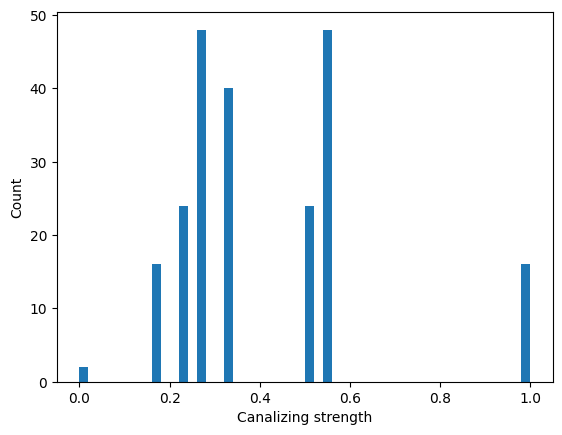
\includegraphics[keepaspectratio]{figures/tutorial03_canalization_fig0.png}}

\subsection{Canalization as a measure of input
redundancy}\label{canalization-as-a-measure-of-input-redundancy}

Canalization, symmetry and redundancy are related concepts. A highly
symmetry Boolean function with few (e.g., one) symmetry groups exhibits
high input redundancy and is on average more canalizing, irrespective of
the measure of canalization. Recently, it was shown that almost all
Boolean functions (except the linear functions) exhibit some level of
\emph{input redundancy} \citep{gates2021effective}. The input redundancy
of a variable is defined as 1 minus its \emph{edge effectiveness}, which
describes the proportion of times that this variable is needed to
determine the output of the function. Edge effectiveness is very similar
to the activity of a variable but is not the same (the difference is
defined as \emph{excess canalization}). The sum of all edge
effectiveness values of the inputs of a function is known as its
\emph{effective degree}. The average input redundancy serves as a
measure of the canalization in a function.

\texttt{BoolForge} can compute all these quantities. To use this
functionality, the optional \texttt{CANA} package must be installed
(\texttt{pip\ install\ cana} or
\texttt{pip\ install\ boolforge{[}cana{]}}). To exemplify this,
reconsider the four 3-input functions from above.

\begin{lstlisting}
for func, label in zip([f, g, h, k], labels):
    edge_eff = func.get_edge_effectiveness()
    activities = func.get_activities()
    effective_degree = func.get_effective_degree()
    input_redundancy = func.get_input_redundancy()

    print(f"Edge effectiveness of {label}: {edge_eff}")
    print(f"Activities of {label}: {activities}")
    print(f"Excess canalization of {label}: {edge_eff - activities}")
    print(f"Effective degree of {label}: {effective_degree}")
    print(f"Average edge effectiveness of {label}: {effective_degree / func.n}")
    print(f"Normalized input redundancy of {label}: {input_redundancy}")
    print()
\end{lstlisting}

\begin{lstlisting}
Edge effectiveness of f: [1.0, 1.0, 1.0]
Activities of f: [1. 1. 1.]
Excess canalization of f: [0. 0. 0.]
Effective degree of f: 3.0
Average edge effectiveness of f: 1.0
Normalized input redundancy of f: 0.0

Edge effectiveness of g: [0.625, 0.625, 0.625]
Activities of g: [0.5 0.5 0.5]
Excess canalization of g: [0.125 0.125 0.125]
Effective degree of g: 1.875
Average edge effectiveness of g: 0.625
Normalized input redundancy of g: 0.375

Edge effectiveness of h: [0.41666666666666663, 0.41666666666666663, 0.41666666666666663]
Activities of h: [0.25 0.25 0.25]
Excess canalization of h: [0.16666667 0.16666667 0.16666667]
Effective degree of h: 1.25
Average edge effectiveness of h: 0.4166666666666667
Normalized input redundancy of h: 0.5833333333333334

Edge effectiveness of k: [0.8125, 0.375, 0.375]
Activities of k: [0.75 0.25 0.25]
Excess canalization of k: [0.0625 0.125  0.125 ]
Effective degree of k: 1.5625
Average edge effectiveness of k: 0.5208333333333334
Normalized input redundancy of k: 0.4791666666666667
\end{lstlisting}

\subsection{Summary}\label{summary-2}

In this tutorial you learned how to:

\begin{itemize}
\tightlist
\item
  compute canalizing depth and identify nested canalizing functions,
\item
  compute the canalizing layer structure and interpret layers and core
  functions,
\item
  quantify collective canalization via \(k\)-set canalizing proportions,
\item
  summarize canalization via canalizing strength,
\item
  relate canalization to redundancy-based measures such as edge
  effectiveness.
\end{itemize}

Canalization provides a structural explanation for why many biological
Boolean rules are robust to perturbations.

Next steps: Subsequent tutorials will explore random Boolean functions
with prescribed canalization properties and the impact of canalization
on Boolean network dynamics and robustness.

\section{Random Boolean function
generation}\label{random-boolean-function-generation}

This tutorial focuses on the random generation of Boolean functions with
prescribed properties, enabling large-scale computational studies.

Controlled random Boolean function generation enables:

\begin{enumerate}
\def\labelenumi{\arabic{enumi}.}
\tightlist
\item
  Null model comparisons: Are biological regulatory rules special?
\item
  Ensemble studies: How do structural properties affect dynamical
  properties?
\item
  Theoretical predictions: Derive expected values for function
  properties
\end{enumerate}

\subsection{What you will learn}\label{what-you-will-learn-3}

In this tutorial you will learn how to generate random Boolean functions
with:

\begin{itemize}
\tightlist
\item
  specified canalizing properties (depth, layer structure),
\item
  bias, absolute bias, or a specific Hamming weight,
\item
  linearity constraints,
\item
  degeneracy constraints.
\end{itemize}

It is strongly recommended to complete the previous tutorials first.

\subsection{Setup}\label{setup-3}

\begin{lstlisting}
import boolforge as bf
import numpy as np
import matplotlib.pyplot as plt
\end{lstlisting}

\subsection{Generating random Boolean
functions}\label{generating-random-boolean-functions}

The function \texttt{random\_function(n,\ *args)} generates a random
\(n\)-input Boolean function subject to optional constraints. By
default, it generates a \emph{non-degenerate} function, meaning that all
variables are essential.

\begin{lstlisting}
n = 3
f = bf.random_function(n)

bf.display_truth_table(f, labels="f_random_non_degenerate")

print("Is f degenerate?", f.is_degenerate())
print("Activities of f:", f.get_activities(exact=True))
print("Edge effectiveness of f:", f.get_edge_effectiveness())
\end{lstlisting}

\begin{lstlisting}
x0  x1  x2  |   f_random_non_degenerate
-------------------------------------------------------
0   0   0   |   0
0   0   1   |   0
0   1   0   |   1
0   1   1   |   0
1   0   0   |   0
1   0   1   |   1
1   1   0   |   1
1   1   1   |   1
Is f degenerate? False
Activities of f: [0.5 0.5 0.5]
Edge effectiveness of f: [0.625, 0.625, 0.75]
\end{lstlisting}

The rest of this tutorial describes the various constraints. Each
constraint defines a specific family of n-input Boolean functions, from
which \texttt{random\_function(n,*args)} samples \emph{uniformly at
random}. That is, each function satisfying a given set of constraints is
selected with equal probability.

\subsection{Parity functions}\label{parity-functions}

Setting \texttt{parity=True} generates \emph{parity} functions, also
known as non-degenerate \emph{linear} functions.

\begin{lstlisting}
f = bf.random_function(n, parity=True)

bf.display_truth_table(f, labels="f_linear")

print("Activities:", f.get_activities(exact=True))
print("Edge effectiveness:", f.get_edge_effectiveness())
print("Normalized average sensitivity:", f.get_average_sensitivity(exact=True))
print("Canalizing strength:", f.get_canalizing_strength())
\end{lstlisting}

\begin{lstlisting}
x0  x1  x2  |   f_linear
----------------------------------------
0   0   0   |   1
0   0   1   |   0
0   1   0   |   0
0   1   1   |   1
1   0   0   |   0
1   0   1   |   1
1   1   0   |   1
1   1   1   |   0
Activities: [1. 1. 1.]
Edge effectiveness: [1.0, 1.0, 1.0]
Normalized average sensitivity: 1.0
Canalizing strength: 0.0
\end{lstlisting}

Parity functions are the only Boolean functions with activity 1 (for all
variables), normalized average sensitivity 1 and canalizing strength 0.

\subsection{Functions with prescribed canalizing
properties}\label{functions-with-prescribed-canalizing-properties}

If \texttt{parity=False} (default), canalizing properties can be
specified via \texttt{layer\_structure} and \texttt{depth}.

\subsubsection{Functions with prescribed canalizing layer
structure}\label{functions-with-prescribed-canalizing-layer-structure}

The canalizing layer structure can be specified via
\texttt{layer\_structure}. This vector describes the number of
conditionally canalizing variables in each layer of the randomly
generated function.

\begin{itemize}
\tightlist
\item
  If the optional argument \texttt{exact\_depth=True} (default is
  False), then \texttt{layer\_structure} describes the \emph{exact}
  layer structure, i.e., the core function cannot be canalizing.
\item
  If \texttt{exact\_depth=False} (the default), it is possible that the
  core function is canalizing (meaning that the last described layer in
  \texttt{layer\_structure} may contain more conditionally canalizing
  variables, or that there are additional canalizing layers).
\end{itemize}

Before generating any random function, \texttt{random\_function()} goes
through a number of checks ensuring that the provided optional arguments
make sense. For example, it checks that the provided layer structure
\((k_1,\ldots,k_r)\) satisfies

\begin{itemize}
\tightlist
\item
  \(k_i\geq 1\),
\item
  \(k_1 + \cdots + k_r \leq n\), and
\item
  if \(k_1 + \cdots + k_r = n\), then \(k_r \geq 2\) because the last
  layer of a nested canalizing function must always contain two or more
  variables.
\end{itemize}

\begin{lstlisting}
f = bf.random_function(n, layer_structure=[1])
g = bf.random_function(n, layer_structure=[1], exact_depth=True)
h = bf.random_function(n, layer_structure=[3])
k = bf.random_function(n, layer_structure=[1, 2])

labels = ["f", "g", "h", "k"]
bf.display_truth_table(f, g, h, k, labels=labels)

for func, label in zip([f, g, h, k], labels):
    info = func.get_layer_structure()
    print(f"Canalizing depth of {label}: {func.get_canalizing_depth()}")
    print(f"Layer structure of {label}: {info['LayerStructure']}")
    print(f"Number of layers of {label}: {info['NumberOfLayers']}")
    print(f"Core function of {label}: {info['CoreFunction']}")
    print()
\end{lstlisting}

\begin{lstlisting}
x0  x1  x2  |   f   g   h   k
---------------------------------------------------------
0   0   0   |   0   1   1   0
0   0   1   |   0   0   1   0
0   1   0   |   0   1   1   1
0   1   1   |   0   1   1   0
1   0   0   |   1   0   1   0
1   0   1   |   0   1   1   0
1   1   0   |   0   1   1   1
1   1   1   |   0   1   0   1
Canalizing depth of f: 3
Layer structure of f: [3]
Number of layers of f: 1
Core function of f: [1]

Canalizing depth of g: 1
Layer structure of g: [1]
Number of layers of g: 1
Core function of g: [1 0 0 1]

Canalizing depth of h: 3
Layer structure of h: [3]
Number of layers of h: 1
Core function of h: [0]

Canalizing depth of k: 3
Layer structure of k: [1, 2]
Number of layers of k: 2
Core function of k: [0]
\end{lstlisting}

Repeated evaluation of this block of code shows that the canalizing
depth of \texttt{f} is either 1 or 3 (note that a canalizing depth of
\(n-1\) is never possible for a non-degenerate function). On the
contrary, the canalizing depth of \texttt{g} is always 1 because we set
\texttt{exact\_depth=True}. The 2-input core function of \texttt{g} is
one of the two parity functions, each with 50\% probability. Likewise,
the core function for the other functions is simply {[}0{]} or {[}1{]},
each with 50\% probability. Functions \texttt{h} and \texttt{k} are
nested canalizing, i.e., their canalizing depth is 3. Their layer
structure is exactly as specified.

\subsubsection{Functions with prescribed canalizing
depth}\label{functions-with-prescribed-canalizing-depth}

If we do not care about the specific layer structure but only about the
canalizing depth, we specify the optional argument \texttt{depth}
instead of \texttt{layer\_structure}.

\begin{lstlisting}

# any function has at least canalizing depth 0 so this is the same as bf.random_function(n)
f = bf.random_function(n,depth=0)


# a random non-canalizing function
g = bf.random_function(n,depth=0,exact_depth=True)


# a random canalizing function
h = bf.random_function(n,depth=1)


# a random nested canalizing function
k = bf.random_function(n,depth=n)

labels = ["f", "g", "h", "k"]
bf.display_truth_table(f, g, h, k, labels=labels)

for func, label in zip([f, g, h, k], labels):
    print(f"Canalizing depth of {label}: {func.get_canalizing_depth()}")
    print()
\end{lstlisting}

\begin{lstlisting}
x0  x1  x2  |   f   g   h   k
---------------------------------------------------------
0   0   0   |   0   0   1   1
0   0   1   |   0   1   1   1
0   1   0   |   0   0   0   1
0   1   1   |   1   0   1   0
1   0   0   |   0   1   1   1
1   0   1   |   1   1   1   1
1   1   0   |   1   1   1   0
1   1   1   |   0   0   0   0
Canalizing depth of f: 0

Canalizing depth of g: 0

Canalizing depth of h: 1

Canalizing depth of k: 3
\end{lstlisting}

Repeated evaluation of this block of code shows that the canalizing
depth of \texttt{f} can be 0, 1, or 3. Note that specifying
\texttt{depth=0} without \texttt{exact\_depth=True} does not restrict
the space of functions at all. On the contrary, the canalizing depth of
\texttt{g} is always 0 (i.e., g does not contain any canalizing
variables) because we set \texttt{exact\_depth=True}. Function
\texttt{h} is canalizing and may be nested canalizing (because we
specified that the minimal canalizing depth is 1), and \texttt{k} is
always nested canalizing (i.e., it has canalizing depth \(n=3\)).

We remember: If \texttt{exact\_depth=True}, \texttt{depth} is
interpreted as exact canalizing depth. Otherwise (default),
\texttt{depth} is interpreted as minimal canalizing depth. For example,

\begin{itemize}
\tightlist
\item
  \texttt{depth=1}: ``At least 1-canalizing'' (could be
  2,3,\ldots,n-canalizing)
\item
  \texttt{depth=1,\ exact\_depth=True}: ``Exactly 1-canalizing'' (not
  2,3,\ldots,n-canalizing)
\end{itemize}

\subsection{Allowing degenerate
functions}\label{allowing-degenerate-functions}

It is possible that an n-input Boolean function does not depend on all
its variables. For example, the function \(f(x,y) = x\) depends on \(x\)
but not on \(y\). \emph{By default, such degenerate functions are never
generated by \texttt{random\_function()}}. To enable the generation of
possibly degenerate functions, we set
\texttt{allow\_degenerate\_functions=True}. Although hardly of any
practical value, we can even restrict the random generation to
degenerate functions only, using
\texttt{bf.generate.random\_degenerate\_function(n,*args)}.

Note: When generating random canalizing functions, the value of
\texttt{allow\_degenerate\_functions} is ignored. The non-canalizing
core function is constructed to depend on all of its variables so that
the number of essential variables equals the specified value. Otherwise
degeneracy would reduce the number of essential variables and confound
analyses of random Boolean networks, especially when the degree is
small.

Since degenerate functions occur much more frequently at low degree, we
set \texttt{n=2}, generate a large number of random, possibly degenerate
functions and compare a histogram of the observed number of essential
variables to the expected proportions.

\begin{lstlisting}
n = 2
n_simulations = 10000

count_essential = np.zeros(n + 1, dtype=int)

for _ in range(n_simulations):
    f = bf.random_function(n, allow_degenerate_functions=True)
    count_essential[f.get_number_of_essential_variables()] += 1

expected = np.array([2 / 16, 4 / 16, 10 / 16])

x = np.arange(n + 1)
width = 0.4

fig, ax = plt.subplots()
ax.bar(x - width / 2, count_essential / n_simulations, width=width, label="observed")
ax.bar(x + width / 2, expected, width=width, label="expected")
ax.legend(frameon=False)
ax.set_xticks(x)
ax.set_xlabel("Number of essential variables")
ax.set_ylabel(f"Proportion of {n}-input functions")

print("Error:", count_essential / n_simulations - expected)
plt.show()
\end{lstlisting}

\begin{lstlisting}
Error: [ 0.0008 -0.0038  0.003 ]
\end{lstlisting}

\pandocbounded{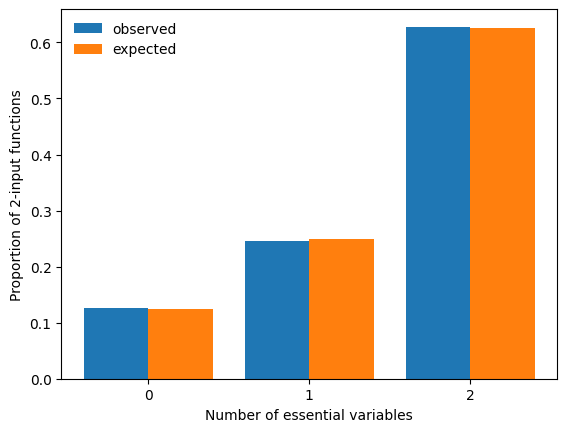
\includegraphics[keepaspectratio]{figures/tutorial04_random_Boolean_function_generation_fig0.png}}

\subsection{Functions with prescribed Hamming
weight}\label{functions-with-prescribed-hamming-weight}

The Hamming weight of a Boolean function is the number of ones in its
truth table. BoolForge allows for the generation of random n-input
functions with a specific Hamming weight \(w\in\{0,1,\ldots,2^n\}\). The
additional optional parameters \texttt{allow\_degenerate\_functions} and
\texttt{exact\_depth} specify whether degenerate and canalizing
functions are allowed. By default, canalizing functions are allowed,
while degenerate functions are not. Since all functions with Hamming
weight \(w\in\{0,1,2^n-1,2^n\}\) are canalizing, we require
\(2\leq w\leq 2^n-2\) whenever canalizing functions are not permissible
(i.e., whenever \texttt{exact\_depth=True}).

\begin{lstlisting}
n = 3

f = bf.random_function(n, hamming_weight=5)
g = bf.random_function(n, hamming_weight=5, exact_depth=True)
h = bf.random_function(n, hamming_weight=2, allow_degenerate_functions=True)

labels = ["f", "g", "h"]
bf.display_truth_table(f, g, h, labels=labels)

for func, label in zip([f, g, h], labels):
    print(f"Hamming weight of {label}: {func.hamming_weight}")
    print(f"Canalizing depth of {label}: {func.get_canalizing_depth()}")
    print(f"Number of essential variables of {label}: {func.get_number_of_essential_variables()}")
    print()
\end{lstlisting}

\begin{lstlisting}
x0  x1  x2  |   f   g   h
-------------------------------------------------
0   0   0   |   1   0   1
0   0   1   |   1   1   0
0   1   0   |   0   1   0
0   1   1   |   1   0   0
1   0   0   |   0   1   0
1   0   1   |   1   0   1
1   1   0   |   0   1   0
1   1   1   |   1   1   0
Hamming weight of f: 5
Canalizing depth of f: 3
Number of essential variables of f: 3

Hamming weight of g: 5
Canalizing depth of g: 0
Number of essential variables of g: 3

Hamming weight of h: 2
Canalizing depth of h: 1
Number of essential variables of h: 3
\end{lstlisting}

\subsection{Biased and absolutely biased
functions}\label{biased-and-absolutely-biased-functions}

While specifying the Hamming weight fixes the exact number of 1s in the
truth table of a generated function, specifying the bias or absolute
bias acts slightly differently. The bias \(p\) describes the probability
of selecting a 1 at any position in the truth table and can be modified
using the optional argument \texttt{bias}. Instead of specifying the
bias, the absolute bias may also be specified. Unbiased functions
contain an equal number of ones and zeros in their truth table and have
an absolute bias of \(0\), the default. If, for example, we set
\texttt{absolute\_bias=0.5} and specify to use absolute bias
(\texttt{use\_absolute\_bias=True}, default is False), the bias used to
generate the function is either 0.25 or 0.75, both with probability
50\%. Generally, if we set
\texttt{use\_absolute\_bias=True;\ absolute\_bias=a} for \(a\in [0,1]\),
the bias is either \((1+a)/2\) or \((1-a)/2\), both with probability
50\%.

To display these different modes, we repeatedly generate random Boolean
functions under three different constraints (\texttt{f} with bias
\(p=0.75\), \texttt{g} with absolute bias 0.5, and \texttt{h} an
unbiased function, i.e., with bias \(p=0.5\)), and compare the empirical
Hamming weight distribution of the three families of functions.

\begin{lstlisting}
n = 4
n_simulations = 10000

counts = np.zeros((3, 2 n + 1), dtype=int)

for _ in range(n_simulations):
    f = bf.random_function(n, bias=0.75)
    g = bf.random_function(n, absolute_bias=0.5, use_absolute_bias=True)
    h = bf.random_function(n, absolute_bias=0.5) #absolute_bias ignored!

    counts[0, f.hamming_weight] += 1
    counts[1, g.hamming_weight] += 1
    counts[2, h.hamming_weight] += 1

labels = ["bias = 0.75", "absolute bias = 0.5", "random (bias = 0.5)"]
x = np.arange(2 n + 1)
width = 0.3

fig, ax = plt.subplots()
for i in range(3):
    ax.bar(x - width + i * width, counts[i] / n_simulations, width=width, label=labels[i])

ax.legend(frameon=False)
ax.set_xticks(x)
ax.set_xlabel("Hamming weight")
ax.set_ylabel(f"Proportion of {n}-input functions")
plt.show()
\end{lstlisting}

\pandocbounded{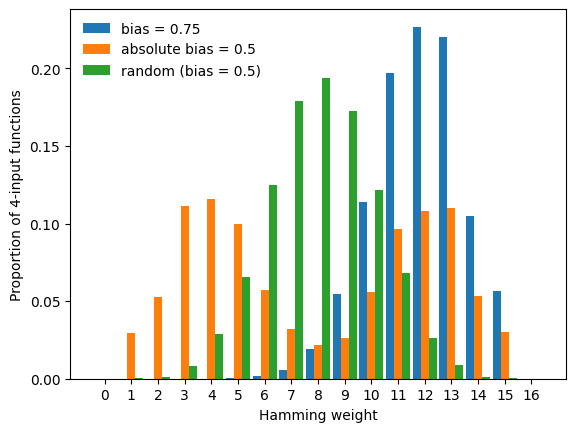
\includegraphics[keepaspectratio]{figures/tutorial04_random_Boolean_function_generation_fig1.png}}

This plot exemplifies the difference between bias and absolute bias:

\begin{itemize}
\tightlist
\item
  Specifying the bias shifts the mode of the Hamming weight distribution
  to the value of \texttt{bias}.
\item
  Specifying the absolute bias yields random functions with a bimodal
  Hamming weight distribution.
\end{itemize}

Note that \texttt{absolute\_bias=0.5} is ignored in the generation of
\texttt{h}. If the value of \texttt{absolute\_bias} should be used, this
must be specified via \texttt{use\_absolute\_bias=True}. By default, the
value of \texttt{bias} (default 0.5) is used.

In the above plot, we notice a lack of functions with Hamming weight 0
and \(16=2^n\). These constant functions are degenerate and thus not
generated unless we set \texttt{allow\_degenerate\_functions=True},
which as we see below, slightly modifies the resulting Hamming weight
distributions.

\begin{lstlisting}
counts[:] = 0

for _ in range(n_simulations):
    f = bf.random_function(
        n, bias=0.75, allow_degenerate_functions=True
    )
    g = bf.random_function(
        n, absolute_bias=0.5, use_absolute_bias=True, allow_degenerate_functions=True
    )
    h = bf.random_function(
        n, allow_degenerate_functions=True
    )

    counts[0, f.hamming_weight] += 1
    counts[1, g.hamming_weight] += 1
    counts[2, h.hamming_weight] += 1

fig, ax = plt.subplots()
for i in range(3):
    ax.bar(x - width + i * width, counts[i] / n_simulations, width=width, label=labels[i])
    
ax.legend(frameon=False)
ax.set_xticks(x)
ax.set_xlabel("Hamming weight")
ax.set_ylabel(f"Proportion of {n}-input functions")
plt.show()
\end{lstlisting}

\pandocbounded{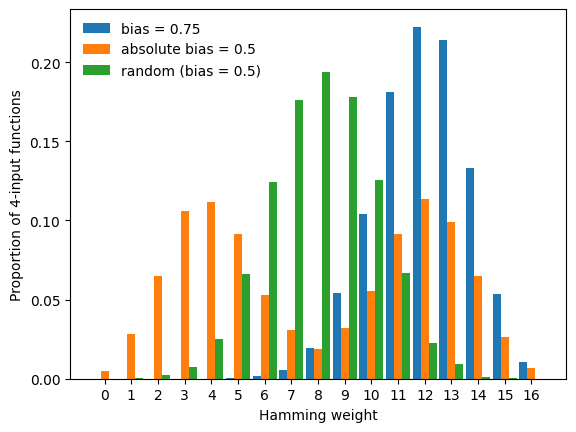
\includegraphics[keepaspectratio]{figures/tutorial04_random_Boolean_function_generation_fig2.png}}

\subsection{Summary}\label{summary-3}

This tutorial demonstrated how BoolForge enables uniform random
generation of Boolean functions under flexible constraints. Different
constraints define fundamentally different ensembles, and being explicit
about these choices is essential for a correct generation and
interpretation of computational results.

Next steps: The next tutorial exemplifies how these function-level
ensembles can be used to uncover new insights into biological regulatory
networks, as well as the relationship between network structure and
dynamics.

\subsection{Common pitfalls}\label{common-pitfalls}

\begin{itemize}
\tightlist
\item
  \texttt{absolute\_bias} has no effect unless
  \texttt{use\_absolute\_bias=True}.
\item
  \texttt{depth=0} without \texttt{exact\_depth=True} does not restrict
  the function space since any Boolean function is at least
  0-canalizing.
\item
  Constant functions and other degenerate functions that do not depend
  on all inputs are only generated if
  \texttt{allow\_degenerate\_functions=True}. If
  \texttt{layer\_structure} or \texttt{depth\textgreater{}0} are
  provided, canalizing functions are generated, which always depend on
  all inputs. That is, in these cases a possible parameter choice of
  \texttt{allow\_degenerate\_functions=True} is ignored.
\item
  For larger \(n\) (e.g., \(n>5\)), set
  \texttt{allow\_degenerate\_functions=True} to avoid expensive
  degeneracy tests. Almost all functions in many variables are
  non-degenerate.
\end{itemize}

\section{Ensemble experiments with random Boolean
functions}\label{ensemble-experiments-with-random-boolean-functions}

In this tutorial, we explore how BoolForge's random Boolean function
generator can be used to generate large ensembles of Boolean functions
with prescribed structural properties, whose statistical and dynamical
characteristics can then be studied.

\subsection{What you will learn}\label{what-you-will-learn-4}

In this tutorial you will learn how to:

\begin{itemize}
\tightlist
\item
  compute the prevalence of canalization, \(k\)-canalization, and nested
  canalization,
\item
  determine distributions of canalizing strength and normalized input
  redundancy,
\item
  investigate correlations between absolute bias and canalization,
\item
  generate and analyze dynamically distinct nested canalizing functions.
\end{itemize}

It is strongly recommended to complete the previous tutorials first.

\subsection{Setup}\label{setup-4}

\begin{lstlisting}
import boolforge as bf
import numpy as np
import matplotlib.pyplot as plt
import pandas as pd
import scipy.stats as stats
\end{lstlisting}

\subsection{Prevalence of
canalization}\label{prevalence-of-canalization}

Using random sampling, we estimate how frequently Boolean functions of
degree \(n\) exhibit a given canalizing depth.

\begin{lstlisting}
n_simulations = 1000
ns = np.arange(2, 7)
canalizing_depths = np.arange(max(ns) + 1)

count_depths = np.zeros((len(ns), max(ns) + 1))

for _ in range(n_simulations):
    for i, n in enumerate(ns):
        f = bf.random_function(n)
        count_depths[i, f.get_canalizing_depth()] += 1

count_depths /= n_simulations

fig, ax = plt.subplots()
for i, depth in enumerate(canalizing_depths):
    ax.bar(
        ns,
        count_depths[:, i],
        bottom=np.sum(count_depths[:, :i], axis=1),
        label=str(depth),
    )

ax.legend(
    frameon=False,
    loc="center",
    bbox_to_anchor=(0.5, 1.1),
    ncol=8,
    title="canalizing depth",
)
ax.set_xticks(ns)
ax.set_xlabel("Number of essential variables")
ax.set_ylabel("Proportion of functions")
plt.show()

out = pd.DataFrame(
    count_depths,
    index=["n=" + str(n) for n in ns],
    columns=["k=" + str(k) for k in canalizing_depths],
)

print(out.to_string())
\end{lstlisting}

\pandocbounded{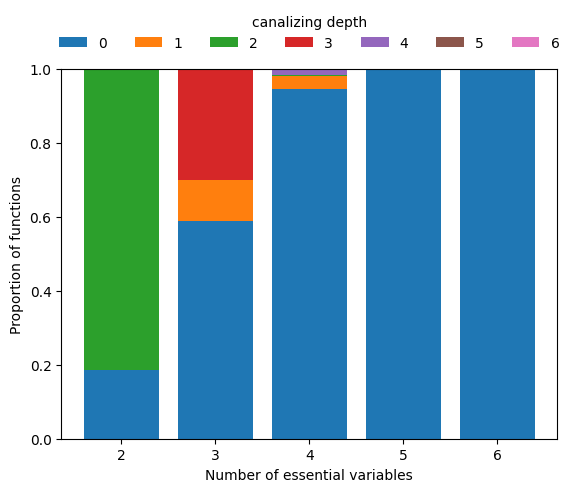
\includegraphics[keepaspectratio]{figures/tutorial05_ensemble_experiments_random_functions_fig5.png}}

\begin{lstlisting}
       k=0    k=1    k=2    k=3    k=4  k=5  k=6
n=2  0.187  0.000  0.813  0.000  0.000  0.0  0.0
n=3  0.590  0.109  0.000  0.301  0.000  0.0  0.0
n=4  0.946  0.035  0.002  0.000  0.017  0.0  0.0
n=5  0.999  0.001  0.000  0.000  0.000  0.0  0.0
n=6  1.000  0.000  0.000  0.000  0.000  0.0  0.0
\end{lstlisting}

We see that hardly any Boolean function with \(n\geq 5\) inputs is
canalizing, let alone nested canalizing. This makes the finding that
most Boolean functions in published Boolean gene regulatory network
models are nested canalizing very surprising \citep{kadelka2024meta}.

\subsubsection{Restricting to canalizing
functions}\label{restricting-to-canalizing-functions}

To zoom in on the few functions that are canalizing for higher \(n\), we
can simply require \texttt{depth=1} and repeat the above analysis.

\begin{lstlisting}
count_depths = np.zeros((len(ns), max(ns) + 1))

for _ in range(n_simulations):
    for i, n in enumerate(ns):
        f = bf.random_function(n, depth=1)
        count_depths[i, f.get_canalizing_depth()] += 1

count_depths /= n_simulations

fig, ax = plt.subplots()
for i, depth in enumerate(canalizing_depths):
    ax.bar(
        ns,
        count_depths[:, i],
        bottom=np.sum(count_depths[:, :i], axis=1),
        label=str(depth),
    )

ax.legend(
    frameon=False,
    loc="center",
    bbox_to_anchor=(0.5, 1.1),
    ncol=8,
    title="canalizing depth",
)
ax.set_xticks(ns)
ax.set_xlabel("Number of essential variables")
ax.set_ylabel("Proportion of functions")
plt.show()

out = pd.DataFrame(
    count_depths,
    index=["n=" + str(n) for n in ns],
    columns=["k=" + str(k) for k in canalizing_depths],
);

print(out.to_string())
\end{lstlisting}

\pandocbounded{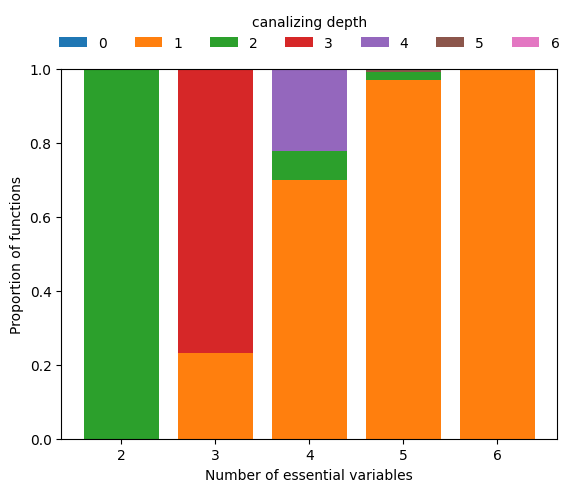
\includegraphics[keepaspectratio]{figures/tutorial05_ensemble_experiments_random_functions_fig6.png}}

\begin{lstlisting}
     k=0    k=1    k=2    k=3    k=4    k=5  k=6
n=2  0.0  0.000  1.000  0.000  0.000  0.000  0.0
n=3  0.0  0.233  0.000  0.767  0.000  0.000  0.0
n=4  0.0  0.700  0.078  0.000  0.222  0.000  0.0
n=5  0.0  0.970  0.022  0.000  0.000  0.008  0.0
n=6  0.0  1.000  0.000  0.000  0.000  0.000  0.0
\end{lstlisting}

This analysis reveals that among Boolean functions of degree
\(n\geq 5\), functions with few conditionally canalizing variables are
much more abundant than functions with more conditionally canalizing
variables, which is mathematically obvious due to the recursive nature
of the definition of k-canalization \citep{he2016stratification}.

\subsection{Collective canalization vs
degree}\label{collective-canalization-vs-degree}

Using a similar setup, we can investigate if and how the various
measures of collective canalization, specifically canalizing strength
\citep{kadelka2023collectively} and the normalized input redundancy
\citep{gates2021effective}, change when the degree of the functions
changes.

\begin{lstlisting}
n_simulations = 100
ns = np.arange(2, 8)

canalizing_strengths = np.zeros((len(ns), n_simulations))
input_redundancies = np.zeros((len(ns), n_simulations))

for j in range(n_simulations):
    for i, n in enumerate(ns):
        f = bf.random_function(n)
        canalizing_strengths[i, j] = f.get_canalizing_strength()
        input_redundancies[i, j] = f.get_input_redundancy()

width = 0.4
fig, ax = plt.subplots()

ax.violinplot(
    canalizing_strengths.T,
    positions=ns - width / 2,
    widths=width,
    showmeans=True,
    showextrema=False,
)
ax.scatter([], [], color="C0", label="canalizing strength")

ax.violinplot(
    input_redundancies.T,
    positions=ns + width / 2,
    widths=width,
    showmeans=True,
    showextrema=False,
)
ax.scatter([], [], color="C1", label="normalized input redundancy")

ax.legend(
    loc="center",
    bbox_to_anchor=(0.5, 1.05),
    frameon=False,
    ncol=2,
)
ax.set_xlabel("Number of essential variables")
ax.set_ylabel("Value")
plt.show()
\end{lstlisting}

\pandocbounded{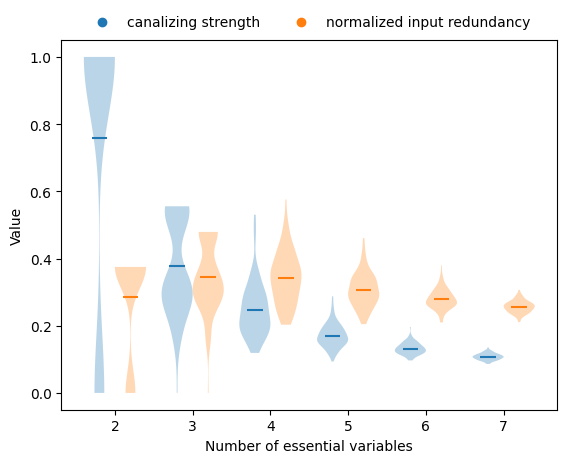
\includegraphics[keepaspectratio]{figures/tutorial05_ensemble_experiments_random_functions_fig7.png}}

Both measures decrease with increasing degree, but canalizing strength
declines more sharply.

\subsubsection{Stratification by canalizing
depth}\label{stratification-by-canalizing-depth}

If we stratify this analysis by canalizing depth (exact canalizing depth
using \texttt{exact\_depth=True} or minimal canalizing depth using the
default \texttt{exact\_depth=False}), we can confirm that functions with
more conditionally canalizing variables tend to also have higher average
collective canalization, irrespective of how it is measured. In other
words, the various measures of canalization are all highly correlated.

\begin{lstlisting}
n_simulations = 100
exact_depth = False
ns = np.arange(2, 7)

max_depth = max(ns)

canalizing_strengths = np.zeros((len(ns), max_depth + 1, n_simulations))
input_redundancies = np.zeros((len(ns), max_depth + 1, n_simulations))

for k in range(n_simulations):
    for i, n in enumerate(ns):
        for depth in np.append(np.arange(n - 1), n):
            f = bf.random_function(n, depth=depth, exact_depth=exact_depth)
            canalizing_strengths[i, depth, k] = f.get_canalizing_strength()
            input_redundancies[i, depth, k] = f.get_input_redundancy()

fig, ax = plt.subplots(2, 1, figsize=(6, 6), sharex=True)

base_gap = 1.0
intra_gap = 0.3
width = 0.28

for ii, (data, label) in enumerate(
    zip(
        [canalizing_strengths, input_redundancies],
        ["canalizing strength", "normalized input redundancy"],
    )
):
    positions = []
    values = []
    colors = []
    group_centers = []

    current_x = 0.0
    for i, n in enumerate(ns):
        depths = np.append(np.arange(n - 1), n)
        offsets = np.linspace(
            -(len(depths) - 1) * intra_gap / 2,
            (len(depths) - 1) * intra_gap / 2,
            len(depths),
        )
        group_positions = current_x + offsets
        positions.extend(group_positions)
        group_centers.append(current_x)

        for d in depths:
            values.append(data[i, d, :])
            colors.append("C" + str(d))

        group_width = (len(depths) - 1) * intra_gap
        current_x += group_width / 2 + base_gap + width + intra_gap

    for pos, val, c in zip(positions, values, colors):
        vp = ax[ii].violinplot(val, positions=[pos], widths=width, showmeans=True, showextrema=False)
        for body in vp["bodies"]:
            body.set_facecolor(c)
            body.set_alpha(0.85)
        vp["cmeans"].set_color("k")

    ax[ii].set_ylabel(label)
    ax[ii].set_ylim([-0.02, 1.02])

ax[1].set_xlabel("Number of essential variables (n)")
ax[1].set_xticks(group_centers)
ax[1].set_xticklabels(ns)

depth_handles = [
    plt.Line2D([0], [0], color="C" + str(d), lw=5, label=str(d))
    for d in range(max_depth + 1)
]

fig.legend(
    handles=depth_handles,
    loc="upper center",
    ncol=7,
    frameon=False,
    title="exact canalizing depth" if exact_depth else "minimal canalizing depth",
)
plt.show()
\end{lstlisting}

\pandocbounded{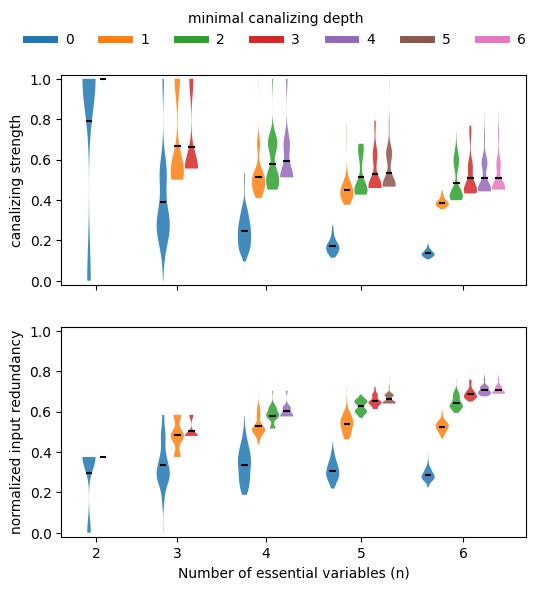
\includegraphics[keepaspectratio]{figures/tutorial05_ensemble_experiments_random_functions_fig0.png}}

\subsubsection{Correlation between canalizing strength and input
redundancy}\label{correlation-between-canalizing-strength-and-input-redundancy}

We can generate all (non-degenerate) Boolean functions of a certain
degree \(n\) (only feasible up to \(n=4\)) and compare canalizing
strength and input redundancy.

\begin{lstlisting}
n = 3
allow_degenerate_functions = False
degenerate = np.zeros(2   (2 n), dtype=bool)
strengths = np.zeros(2   (2 n))
redundancies = np.zeros(2   (2 n))

for i, fvec in enumerate(bf.get_left_side_of_truth_table(2 n)):
    f = bf.BooleanFunction(fvec)
    strengths[i] = f.get_canalizing_strength()
    redundancies[i] = f.get_input_redundancy()
    if not allow_degenerate_functions:
        degenerate[i] = f.is_degenerate()
        
if allow_degenerate_functions:
    which = np.ones(2   (2 n), dtype=bool)
else:
    which = ~degenerate
    

plt.figure(figsize=(5, 4))
plt.scatter(strengths[which], redundancies[which], alpha=0.7)
plt.xlabel("Canalizing strength")
plt.ylabel("Normalized input redundancy")
plt.tight_layout()
plt.show()

stats.spearmanr(strengths[which], redundancies[which])
\end{lstlisting}

\pandocbounded{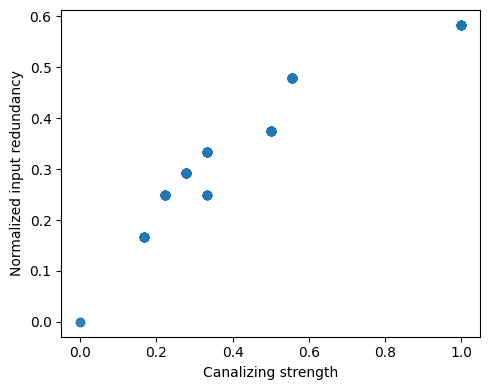
\includegraphics[keepaspectratio]{figures/tutorial05_ensemble_experiments_random_functions_fig1.png}}

\begin{lstlisting}
SignificanceResult(statistic=np.float64(0.9700304760700043), pvalue=np.float64(1.0759731607818433e-134))
\end{lstlisting}

Both measures are highly correlated but markedly not the same, which
becomes even more evident when rerunning the analysis for \(n=4\) (see
\citet{kadelka2026canalization}). Some functions possess relatively high
canalizing strength but low input redundancy, and vice versa. It remains
an open question what drives this behavior.

\subsection{Correlation between canalization and
bias}\label{correlation-between-canalization-and-bias}

All metrics used to assess the sensitivity of Boolean functions
(canalization, absolute bias, average sensitivity) are correlated. For
example, functions with higher absolute bias are more likely to be
canalizing.

\begin{lstlisting}
ns = np.arange(2, 6)
n_simulations = 3000
bias_values = np.linspace(0, 1, 21)

count_canalizing = np.zeros((len(ns), len(bias_values)), dtype=int)

for i, n in enumerate(ns):
    for _ in range(n_simulations):
        for j, bias in enumerate(bias_values):
            f = bf.random_function(n, bias=bias, allow_degenerate_functions=True)
            if f.is_canalizing():
                count_canalizing[i, j] += 1

fig, ax = plt.subplots()
for i, n in enumerate(ns):
    ax.plot(bias_values, count_canalizing[i] / n_simulations, label=f"n={n}")

xticks = [0, 0.25, 0.5, 0.75, 1]
ax.set_xticks(xticks)
ax.set_xticklabels([f"{p} ({round(200*abs(p-0.5))}%)" for p in xticks])
ax.set_xlabel("bias (absolute bias)")
ax.set_ylabel("probability canalizing")
ax.legend(
    loc="center",
    frameon=False,
    bbox_to_anchor=(0.5, 1.05),
    ncol=6,
)
plt.show()
\end{lstlisting}

\pandocbounded{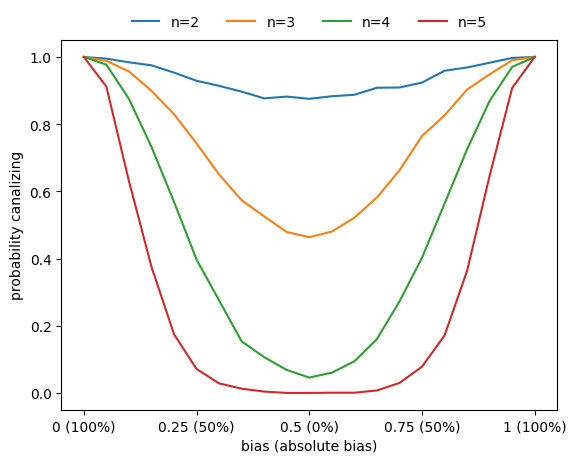
\includegraphics[keepaspectratio]{figures/tutorial05_ensemble_experiments_random_functions_fig2.png}}

\subsubsection{Degeneracy vs bias}\label{degeneracy-vs-bias}

Similarly, the probability that a function is degenerate (i.e., that it
does not depend on all its variables) also increases as the absolute
bias increases.

\begin{lstlisting}
count_degenerate = np.zeros((len(ns), len(bias_values)), dtype=int)

for i, n in enumerate(ns):
    for _ in range(n_simulations):
        for j, bias in enumerate(bias_values):
            f = bf.random_function(n, bias=bias, allow_degenerate_functions=True)
            if f.is_degenerate():
                count_degenerate[i, j] += 1

fig, ax = plt.subplots()
for i, n in enumerate(ns):
    ax.plot(bias_values, count_degenerate[i] / n_simulations, label=f"n={n}")

ax.set_xticks(xticks)
ax.set_xticklabels([f"{p} ({round(200*abs(p-0.5))}%)" for p in xticks])
ax.set_xlabel("bias (absolute bias)")
ax.set_ylabel("probability degenerate")
ax.legend(
    loc="center",
    frameon=False,
    bbox_to_anchor=(0.5, 1.05),
    ncol=6,
)
plt.show()
\end{lstlisting}

\pandocbounded{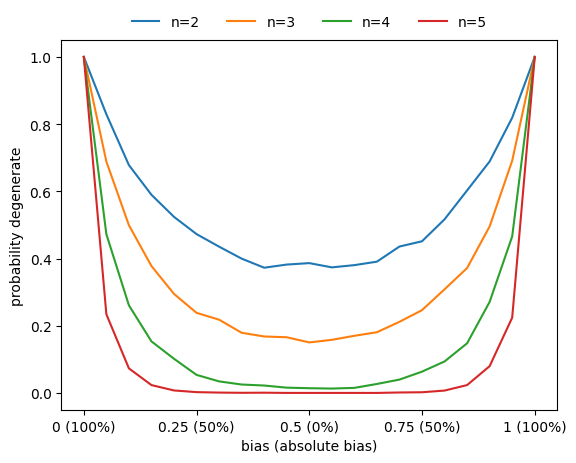
\includegraphics[keepaspectratio]{figures/tutorial05_ensemble_experiments_random_functions_fig3.png}}

\subsection{Analyzing functions with specific canalizing layer
structure}\label{analyzing-functions-with-specific-canalizing-layer-structure}

The average sensitivity of the Boolean functions governing the updates
in a Boolean network, determines the stability of the network to
perturbations. More generally, it determines the dynamical regime of the
network (see Tutorial 8). The ability to generate canalizing functions
with a specific canalizing layer structure enables us to investigate the
link between layer structure and average sensitivity, as well as other
properties, such as canalizing strength or effective degree.

For nested canalizing functions of a given degree \(n\), there exists a
bijection between their absolute bias and their canalizing layer
structure \citep{kadelka2017influence}. The function
\texttt{boolforge.hamming\_weight\_to\_ncf\_layer\_structure(degree,hamming\_weight)}
implements this. NCFs with the same layer structure have the same
dynamical properties. That is, they have the same average sensitivity,
canalizing strength and the same effective degree. Iterating over all
possible absolute biases (parametrized by the possible Hamming weights),
we can thus generate all dynamically different types of n-input NCFs and
investigate their average sensitivity, which we can compute exactly for
relatively low degree.

\begin{lstlisting}
n = 5
all_hamming = np.arange(1, 2   (n - 1), 2)
all_abs_bias = 2 * np.abs(all_hamming/2 n - 0.5)

avg_sens = np.zeros(2   (n - 2))
can_strength = np.zeros_like(avg_sens)
eff_degree = np.zeros_like(avg_sens)
layer_structures = []

for i, w in enumerate(all_hamming):
    layer = bf.hamming_weight_to_ncf_layer_structure(n, w)
    layer_structures.append(layer)
    f = bf.random_function(n, layer_structure=layer)
    avg_sens[i] = f.get_average_sensitivity(exact=True, normalized=False)
    can_strength[i] = f.get_canalizing_strength()
    eff_degree[i] = f.get_effective_degree()

df = pd.DataFrame(
    {
        "Hamming weight": all_hamming,
        "Absolute bias": all_abs_bias,
        "Layer structure": list(map(str, layer_structures)),
        "Average sensitivity": avg_sens,
        "Canalizing strength": np.round(can_strength, 4),
        "Effective degree": np.round(eff_degree, 4),
    }
)

print(df.to_string())
\end{lstlisting}

\begin{lstlisting}
   Hamming weight  Absolute bias Layer structure  Average sensitivity  Canalizing strength  Effective degree
0               1         0.9375             [5]               0.3125               1.0000            1.1250
1               3         0.8125          [3, 2]               0.6875               0.7705            1.3984
2               5         0.6875       [2, 1, 2]               0.9375               0.6369            1.5938
3               7         0.5625          [2, 3]               1.0625               0.5993            1.5833
4               9         0.4375       [1, 1, 3]               1.1875               0.5033            1.7266
5              11         0.3125    [1, 1, 1, 2]               1.3125               0.4657            1.8021
6              13         0.1875       [1, 2, 2]               1.3125               0.4657            1.7708
7              15         0.0625          [1, 4]               1.1875               0.5033            1.6094
\end{lstlisting}

We notice that nested canalizing functions with higher absolute bias
tend to be more sensitive to input changes and also less canalizing.
However, the relationship between absolute bias and these other metrics
is far from monotonic. Further, we notice that there is a perfect
correlation between the average sensitivity of a nested canalizing
function and its canalizing strength, and a near perfect correlation
between average sensitivity and effective degree.

To investigate the non-monotonic behavior further, we can vary the
degree and create line plots that reveal a clear pattern, as shown in
\citet{kadelka2017influence}.

\begin{lstlisting}
ns = np.arange(5, 9)
fig, ax = plt.subplots()

for n in ns:
    all_hamming_weights = np.arange(1, 2   (n - 1), 2)
    all_abs_bias = 2 * np.abs(all_hamming_weights/2 n - 0.5)
    avg_sens = np.zeros(2   (n - 2))

    for i, w in enumerate(all_hamming_weights):
        layer = bf.hamming_weight_to_ncf_layer_structure(n, w)
        f = bf.random_function(n, layer_structure=layer)
        avg_sens[i] = f.get_average_sensitivity(exact=True, normalized=False)

    ax.plot(all_abs_bias, avg_sens, "x--", label=f"n={n}")

ax.legend(frameon=False)
ax.set_xlabel("Absolute bias")
ax.set_ylabel("Average sensitivity")
plt.show()
\end{lstlisting}

\pandocbounded{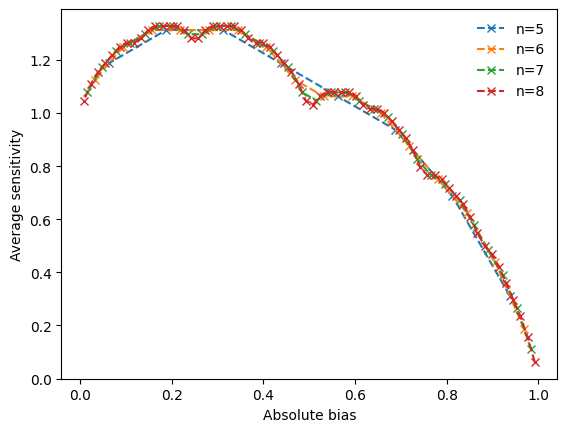
\includegraphics[keepaspectratio]{figures/tutorial05_ensemble_experiments_random_functions_fig4.png}}

\subsection{Summary}\label{summary-4}

This tutorial illustrated how ensembles of Boolean functions generated
under explicit constraints reveal systematic relationships between
canalization, bias, redundancy, and sensitivity.

The key findings include:

\begin{enumerate}
\def\labelenumi{\arabic{enumi}.}
\tightlist
\item
  Canalization is rare in random functions but common in biology.
\item
  Canalizing strength and input redundancy both decrease with degree.
\item
  Functions with high absolute bias are more likely to be highly
  canalizing.
\item
  For NCFs, layer structure is uniquely determined by bias.
\item
  Average sensitivity varies systematically with layer structure.
\end{enumerate}

These relationships constrain the space of biologically plausible
functions and suggest evolutionary optimization for robustness.

We now move on to Boolean networks, where Boolean functions serve as
node update rules and give rise to collective dynamical behavior.

\section{Working with Boolean
Networks}\label{working-with-boolean-networks}

While previous tutorials focused on individual Boolean functions, this
tutorial introduces Boolean networks, which combine multiple Boolean
functions into a dynamical system.

\subsection{What you will learn}\label{what-you-will-learn-5}

In this tutorial you will learn how to:

\begin{itemize}
\tightlist
\item
  create Boolean networks,
\item
  compute basic properties of the wiring diagram,
\item
  compute basic properties of Boolean networks.
\item
  transform Boolean networks through structural manipulations such as
  fixing node values or removing regulatory interactions.
\end{itemize}

\subsection{Setup}\label{setup-5}

\begin{lstlisting}
import boolforge as bf
import numpy as np
\end{lstlisting}

\subsection{Boolean network theory}\label{boolean-network-theory}

A Boolean network \(F = (f_1, \ldots, f_N)\) is a dynamical system
consisting of \(N\) Boolean update functions. Each node can be in one of
two states, 0 or 1, often interpreted as OFF/ON in biological contexts.

Under \emph{synchronous updating}, all nodes update simultaneously,
yielding a deterministic state transition graph on \(\{0,1\}^N\). Under
\emph{asynchronous updating}, only one node is updated at a time,
yielding a stochastic transition graph. BoolForge implements both
schemes.

Real biological networks are typically sparsely connected. The
\emph{in-degree} of a node is the number of essential inputs of its
update function. The \emph{wiring diagram} encodes which nodes regulate
which others.

Despite their simplicity, Boolean networks can:

\begin{itemize}
\tightlist
\item
  reproduce complex dynamics (oscillations, multistability),
\item
  predict gene knockout effects,
\item
  identify control strategies,
\item
  scale to genome-wide networks (1000s of nodes).
\end{itemize}

\subsection{Wiring diagrams}\label{wiring-diagrams}

We first construct wiring diagrams, which encode network structure
independently of specific Boolean functions. Separating topology
(encoded in BoolForge by \texttt{I}) from dynamics (\texttt{F}) allows:

\begin{itemize}
\tightlist
\item
  studying structural properties independent of specific Boolean rules,
\item
  swapping different rule sets on the same topology,
\item
  efficient storage (sparse I, local F vs dense full truth table).
\end{itemize}

\begin{lstlisting}

# Wiring diagram of a 3-node network
I = [
    [1],
    [0, 2],
    [1],
]

W = bf.WiringDiagram(I=I)

print("W.N:", W.N)
print("W.variables:", W.variables)
print("W.indegrees:", W.indegrees)
print("W.outdegrees:", W.outdegrees)

fig = W.plot(show=False);
\end{lstlisting}

\begin{lstlisting}
W.N: 3
W.variables: ['x0' 'x1' 'x2']
W.indegrees: [1 2 1]
W.outdegrees: [1 2 1]
\end{lstlisting}

\pandocbounded{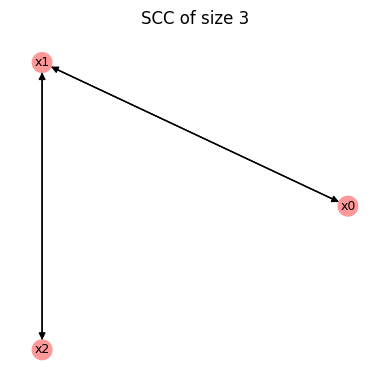
\includegraphics[keepaspectratio]{figures/tutorial06_boolean_networks_fig4.png}}

The wiring diagram above consists of \(N=3\) variables, and uses default
variable names \(x_0, \ldots, x_{N-1}\). The vectors \texttt{indegrees}
and \texttt{outdegrees} describe the number of incoming and outgoing
edges for each node.

\subsubsection{Example with constants and unequal
degrees}\label{example-with-constants-and-unequal-degrees}

The next wiring diagram contains a constant node (source) \(x_0\) and a
node that is only regulated but does not regulate any nodes (sink)
\(x_2\).

\begin{lstlisting}
I = [
    [],
    [0],
    [0, 1], 
]

W = bf.WiringDiagram(I=I)

print("W.N:", W.N)
print("W.variables:", W.variables)
print("W.indegrees:", W.indegrees)
print("W.outdegrees:", W.outdegrees)

fig = W.plot(show=False)
\end{lstlisting}

\begin{lstlisting}
W.N: 3
W.variables: ['x0' 'x1' 'x2']
W.indegrees: [0 1 2]
W.outdegrees: [2 1 0]
\end{lstlisting}

\pandocbounded{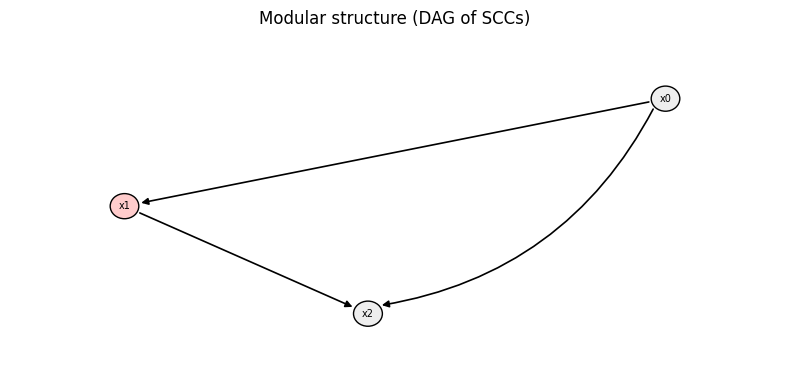
\includegraphics[keepaspectratio]{figures/tutorial06_boolean_networks_fig5.png}}

This wiring diagram encodes a \emph{feed-forward loop}, one of the most
common \emph{network motifs} in transcriptional networks. It can:

\begin{itemize}
\tightlist
\item
  filter transient signals (coherent FFL with AND gate),
\item
  accelerate response (incoherent FFL),
\end{itemize}

See \citet{mangan2003structure} for a detailed analysis.
\texttt{BoolForge} enables the identification of all feed-forward loops:

\begin{lstlisting}
print("W.get_ffls()", W.get_ffls())
\end{lstlisting}

\begin{lstlisting}
W.get_ffls() {'FFLs': [[0, 1, 2]]}
\end{lstlisting}

This tells us that \texttt{W} contains one FFL, in which \(x_0\)
regulates both \(x_1\) and \(x_2\), while \(x_2\) is also regulated by
\(x_1\).

\texttt{BoolForge} can also identify all feedback loops. For this, we
consider another wiring diagram:

\begin{lstlisting}
I2 = [
    [2,1],
    [0],
    [1],
]

W2 = bf.WiringDiagram(I=I2)
fig = W2.plot(show=False)
fig

print("W2.get_fbls()", W2.get_fbls())
\end{lstlisting}

\begin{lstlisting}
W2.get_fbls() {'FBLs': [[0, 1, 2], [0, 1]]}
\end{lstlisting}

\pandocbounded{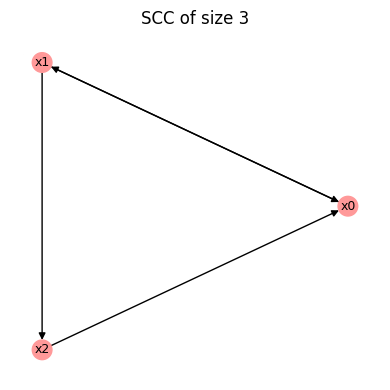
\includegraphics[keepaspectratio]{figures/tutorial06_boolean_networks_fig0.png}}

The function \texttt{.get\_fbls()} identifies all simple cycles in the
wiring diagram. In this case, there exists a 2-cycle
\(x_0 \leftrightarrow x_1\) and a 3-cycle
\(x_0 \to x_1 \to x_2 \to x_0\).

\subsection{Creating Boolean networks}\label{creating-boolean-networks}

To create a Boolean network, we must specify:

\begin{enumerate}
\def\labelenumi{\arabic{enumi}.}
\tightlist
\item
  A wiring diagram \texttt{I}, describing who regulates whom.
\item
  A list \texttt{F} of Boolean update functions (or truth tables), one
  per node.
\end{enumerate}

\begin{lstlisting}
I = [
    [1],
    [0, 2],
    [1],
]

F = [
    [0, 1],
    [0, 1, 1, 1],
    [0, 1],
]

bn = bf.BooleanNetwork(F=F, I=I)

print(bn.to_truth_table().to_string())
\end{lstlisting}

\begin{lstlisting}
   x0(t)  x1(t)  x2(t)  x0(t+1)  x1(t+1)  x2(t+1)
0      0      0      0        0        0        0
1      0      0      1        0        1        0
2      0      1      0        1        0        1
3      0      1      1        1        1        1
4      1      0      0        0        1        0
5      1      0      1        0        1        0
6      1      1      0        1        1        1
7      1      1      1        1        1        1
\end{lstlisting}

The full truth table of a Boolean network has size \(N \times 2^N\) and
therefore grows exponentially with the number of nodes.\\
In practice, however, \texttt{BoolForge} never stores this object
explicitly. Instead, a Boolean network is represented internally by its
wiring diagram \texttt{I} and the list of update functions \texttt{F},
which is far more memory-efficient -- especially for sparse networks
with few regulators per node.

When a Boolean network is constructed from \texttt{F} and \texttt{I},
\texttt{BoolForge} automatically performs a series of consistency checks
to guard against common modeling errors. For example, it verifies that
each update function has the correct length, namely \(2^n\), where \(n\)
is the number of regulators of the corresponding node as specified in
\texttt{I}. If any of these checks fail, an informative error is raised
immediately, helping ensure that the resulting network is well-defined.

\subsubsection{Creating networks from
strings}\label{creating-networks-from-strings}

Alternatively, Boolean networks can be specified using a human-readable
string representation, where each line defines the update rule of one
node. This format closely mirrors the way Boolean models are written in
the literature and is often more convenient than manually specifying
wiring diagrams and truth tables.

In the example below, each line has the form
\(x_i = f_i(\text{regulators of } x_i),\) where Boolean operators such
as \texttt{AND}, \texttt{OR}, and \texttt{NOT} can be used to define the
update functions.

\begin{lstlisting}
string = """
x = y
y = x OR z
z = y
"""

bn_str = bf.BooleanNetwork.from_string(string, separator="=")
print(bn_str.to_truth_table().to_string())
\end{lstlisting}

\begin{lstlisting}
   x(t)  y(t)  z(t)  x(t+1)  y(t+1)  z(t+1)
0     0     0     0       0       0       0
1     0     0     1       0       1       0
2     0     1     0       1       0       1
3     0     1     1       1       1       1
4     1     0     0       0       1       0
5     1     0     1       0       1       0
6     1     1     0       1       1       1
7     1     1     1       1       1       1
\end{lstlisting}

Here, the update rule \texttt{x\ =\ y} specifies that node \texttt{x}
copies the state of \texttt{y}, while \texttt{y\ =\ x\ OR\ z} indicates
that node \texttt{y} becomes activated (1) whenever \texttt{x}, or
\texttt{z}, or both are active.

From this symbolic description, \texttt{BoolForge} automatically:

\begin{itemize}
\tightlist
\item
  extracts the wiring diagram,
\item
  determines the regulators of each node,
\item
  constructs the corresponding Boolean update functions.
\end{itemize}

Internally, the string representation is converted into the same
\texttt{(F,\ I)} representation used throughout the package. As a
result, Boolean networks created from strings behave identically to
those created explicitly from wiring diagrams and truth tables.

This interface is particularly useful for loading Boolean network models
from external sources, such as \texttt{.bnet} files, or for quickly
prototyping models in an interactive setting.

\subsubsection{Interoperability with
CANA}\label{interoperability-with-cana}

\texttt{BoolForge} provides native interoperability with the
\href{https://www.github.com/CASCI-lab/CANA}{CANA package} for the
analysis of Boolean functions and Boolean networks
\citep{marcus2025cana}. Existing \texttt{BoolForge} networks can be
converted into \texttt{CANA} objects and back without loss of
information.

In the example below, we convert a \texttt{BoolForge} Boolean network
into its \texttt{CANA} representation using \texttt{to\_cana()}, and
then reconstruct a new \texttt{BoolForge} Boolean network from that
\texttt{CANA} object.

The final assertion verifies that this round-trip conversion preserves:

\begin{itemize}
\tightlist
\item
  the Boolean update functions,
\item
  the wiring diagram,
\item
  and the variable names.
\end{itemize}

This guarantees that \texttt{BoolForge} and \texttt{CANA} can be used
interchangeably within a workflow, allowing users to leverage
\texttt{CANA}'s analytical tools while continuing to build and
manipulate models using \texttt{BoolForge}.

\begin{lstlisting}
cana_bn = bn.to_cana()
bn_from_cana = bf.BooleanNetwork.from_cana(cana_bn)

assert (
    np.all([np.all(bn.F[i].f == bn_from_cana.F[i].f) for i in range(bn.N)])
    and np.all([np.all(bn.I[i] == bn_from_cana.I[i]) for i in range(bn.N)])
    and np.all(bn.variables == bn_from_cana.variables)
), "BooleanNetwork CANA conversion failed"
\end{lstlisting}

\subsection{Types of nodes in Boolean
networks}\label{types-of-nodes-in-boolean-networks}

Nodes in a Boolean network can be classified as follows:

\begin{itemize}
\tightlist
\item
  \emph{Constant nodes}:\\
  Nodes with constant update functions (always 0 or always 1). These
  nodes act as parameters and they are eliminated at construction time
  by substituting their constant value into all dependent update
  functions.
\item
  \emph{Identity nodes}:\\
  Nodes whose update function is the identity, i.e., \(f(x_i) = x_i.\)
  Their value is determined by the initial condition and remains
  constant over time. Identity nodes are retained as part of the Boolean
  network state. They may be viewed as nodes with a self-loop and no
  other incoming edges.
\item
  \emph{Regulated nodes}:\\
  Nodes whose update functions depend on one or more other nodes.
\end{itemize}

\begin{lstlisting}
F = [
    [0, 0, 0, 1],  # regulated
    [0, 1, 1, 1],  # regulated
    [0, 1],        # identity
    [0],           # constant
]

I = [
    [1, 2],        # regulated
    [0, 3],        # regulated
    [2],           # identity
    [],            # constant
]

bn = bf.BooleanNetwork(F, I)

print("bn.variables:", bn.variables)
print("bn.constants:", bn.constants)
print("bn.I:", bn.I)
print("bn.F:")
for i, f in enumerate(bn.F):
    print(f"  F[{i}] = {f!r}")
\end{lstlisting}

\begin{lstlisting}
bn.variables: ['x0' 'x1' 'x2']
bn.constants: {'x3': 0}
bn.I: [array([1, 2]), array([0]), array([2])]
bn.F:
  F[0] = BooleanFunction(name='x0', f=[0, 0, 0, 1])
  F[1] = BooleanFunction(name='x1', f=[0, 1])
  F[2] = BooleanFunction(name='x2', f=[0, 1])
\end{lstlisting}

The constant node is removed, and its value is propagated into
downstream update functions.

If we now change the value of the constant node from 0 to 1, the network
is constructed in the same way, and the constant value 1 is substituted
directly into all downstream update functions, before removal of the
constant node.

As a result, the Boolean update functions of downstream nodes may
simplify, potentially reducing the number of regulators or changing the
logical form of the function. This illustrates how constant nodes act as
parameters whose values influence the effective dynamics of the network.

Importantly, this simplification is performed symbolically at
construction time and does not depend on the dynamical evolution of the
network.

\begin{lstlisting}
F = [
    [0, 0, 0, 1],
    [0, 1, 1, 1],
    [0, 1],
    [1],
]

I = [
    [1, 2],
    [0, 3],
    [2],
    [],
]

bn = bf.BooleanNetwork(F, I)

print("bn.variables:", bn.variables)
print("bn.constants:", bn.constants)
print("bn.I:", bn.I)
print("bn.F:")
for i, f in enumerate(bn.F):
    print(f"  F[{i}] = {f!r}")
\end{lstlisting}

\begin{lstlisting}
bn.variables: ['x0' 'x1' 'x2']
bn.constants: {'x3': 1}
bn.I: [array([1, 2]), array([0]), array([2])]
bn.F:
  F[0] = BooleanFunction(name='x0', f=[0, 0, 0, 1])
  F[1] = BooleanFunction(name='x1', f=[1, 1])
  F[2] = BooleanFunction(name='x2', f=[0, 1])
\end{lstlisting}

Although \(x_1\) becomes fixed at 1 after one update, it is not treated
as a constant node. In \texttt{BoolForge}, constant nodes are identified
by their update functions (always 0 or always 1), not by their long-term
dynamical behavior. In other words, BoolForge distinguishes structural
constants (defined by update rules) from dynamical constants (states
that become fixed along trajectories). Since \(x_1 = 0\) remains a valid
initial condition, the node is retained as part of the network state.

\subsection{Boolean network
properties}\label{boolean-network-properties}

The class \texttt{BooleanNetwork} inherits basic structural properties
and methods from \texttt{WiringDiagram}. In particular, all
graph-theoretic attributes of the wiring diagram -- such as the number
of nodes, in-degrees, and out-degrees -- are directly accessible on a
Boolean network object.

Moreover, \texttt{BooleanNetwork} inherits visualization utilities from
\texttt{WiringDiagram}, including methods for plotting the wiring
diagram and its modular structure, using \texttt{.plot()}. This allows
users to inspect the topology of a Boolean network independently of the
specific update functions.

Beyond these inherited features, \texttt{BooleanNetwork} provides a rich
collection of additional methods for analyzing the dynamics, structure,
and control properties of Boolean networks. These include functionality
for:

\begin{itemize}
\tightlist
\item
  computing fixed points and attractors,
\item
  analyzing transient dynamics and state transition graphs,
\item
  studying robustness and sensitivity to perturbations,
\item
  performing node and edge interventions.
\end{itemize}

Many of these methods will be introduced and discussed in detail in the
following tutorials. Here, we focus only on a few basic and commonly
used properties.

\begin{lstlisting}
print("bn.N:", bn.N)
print("bn.indegrees:", bn.indegrees)
print("bn.outdegrees:", bn.outdegrees)
print("bn.variables:", bn.variables)

bn.plot();
\end{lstlisting}

\begin{lstlisting}
bn.N: 3
bn.indegrees: [2 1 1]
bn.outdegrees: [1 1 2]
bn.variables: ['x0' 'x1' 'x2']
\end{lstlisting}

\pandocbounded{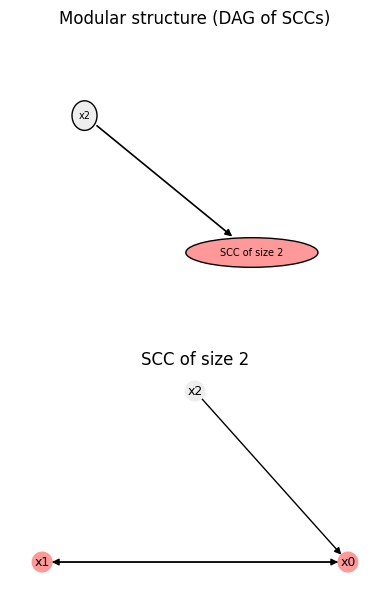
\includegraphics[keepaspectratio]{figures/tutorial06_boolean_networks_fig1.png}}

Just like BooleanFunction objects, BooleanNetwork possesses a
\texttt{.summary()} method, which prints a human-readable overview of
basic properties. If more advanced properties have already been
computed, e.g., attractors, this information is also displayed (or if
the optional keyword \texttt{compute\_all} is set to True, default
False).

\begin{lstlisting}
print(bn.summary())
print()
print(bn.summary(compute_all=True)) #or simply print(bn.summary(True))
\end{lstlisting}

\begin{lstlisting}
BooleanNetwork
--------------
Number of nodes:              3
Number of regulated nodes:    2
Number of identity nodes:     1
Number of constants (removed):1
Average degree:               1.333
Largest in-degree:            2
Largest out-degree:           2
Regulated nodes:              ['x0', 'x1']
Identity nodes (inputs):      ['x2']
Constants:                    {'x3': 1}

BooleanNetwork
--------------
Number of nodes:              3
Number of regulated nodes:    2
Number of identity nodes:     1
Number of constants (removed):1
Average degree:               1.333
Largest in-degree:            2
Largest out-degree:           2
Regulated nodes:              ['x0', 'x1']
Identity nodes (inputs):      ['x2']
Constants:                    {'x3': 1}
Number of attractors:         2
Largest basin size:           0.500
Basin size entropy:           0.693
Derrida value:                0.667
Coherence:                    0.667
Fragility:                    0.222
\end{lstlisting}

The more advanced properties displayed here are the subject of the next
two tutorials.

\subsection{Manipulation and control of Boolean
networks}\label{manipulation-and-control-of-boolean-networks}

Identity nodes can represent external inputs or environmental
conditions. Fixing their values allows us to study the behavior of the
network under specific contexts. BoolForge enables users to obtain a
reduced network, in which the identity nodes are set to specific values.

\begin{lstlisting}
cn = bn.get_network_with_fixed_identity_nodes(values_identity_nodes=[0])
print("cn.F:")
for i, f in enumerate(cn.F):
    print(f"  F[{i}] = {f!r}")
print()
print(cn.summary())
\end{lstlisting}

\begin{lstlisting}
cn.F:
  F[0] = BooleanFunction(name='x0', f=[0, 0])
  F[1] = BooleanFunction(name='x1', f=[1, 1])

BooleanNetwork
--------------
Number of nodes:              2
Number of regulated nodes:    2
Number of constants (removed):2
Average degree:               1.000
Largest in-degree:            1
Largest out-degree:           1
Regulated nodes:              ['x0', 'x1']
Constants:                    {'x2': 0, 'x3': 1}
\end{lstlisting}

Fixing identity nodes converts them into constant nodes, which are then
eliminated via constant propagation. Only the identity nodes are removed
from \texttt{cn}. Nodes that become dynamically constant after fixing
identity nodes (e.g., \(x_0\) and \(x_1\)) are retained, since their
initial values may still vary. For example, \(x_0(t=0) = 1\) or
\(x_1(t=0) = 0\) remain valid initial values, despite the fact that
\(x_0(t) = 0\) and \(x_1(t) = 1\) at any time \(t>0\).

\subsubsection{Node controls}\label{node-controls}

Boolean network control is an active area of research (see e.g.,
\citet{murrugarra2016identification} or \citet{borriello2021basis}). For
example, the knock-out of a certain gene can be simulated in a Boolean
network by setting this gene to a constant value of zero. Likewise,
overexpression can be modeled by setting it to a constant value of one.
BoolForge enables users to implement node and edge controls of existing
Boolean networks. This provides a simple framework for simulating
interventions such as gene knock-outs or overexpression.

To implement node controls, we need to specify which nodes should be
controlled and the constant values that they should be set to. As an
example, we consider a classical Boolean network model, the three-node
repressilator \citep{elowitz2000synthetic}.

\begin{lstlisting}
string = """
A = not B
B = not C
C = not A
"""

bn = bf.BooleanNetwork.from_string(string, separator="=")
bn.plot();
cn = bn.get_network_with_node_controls(indices_controlled_nodes=[2],
                                       values_controlled_nodes=[0])
cn.plot();
print("cn.F:")
for i, f in enumerate(cn.F):
    print(f"  F[{i}] = {f!r}")
print("cn.constants:", cn.constants)
\end{lstlisting}

\pandocbounded{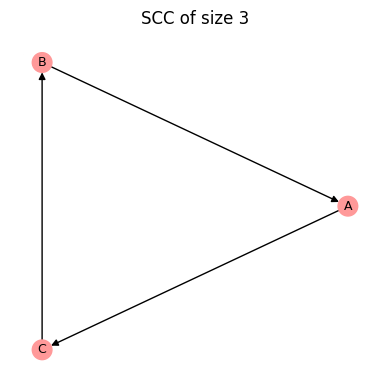
\includegraphics[keepaspectratio]{figures/tutorial06_boolean_networks_fig2.png}}

\pandocbounded{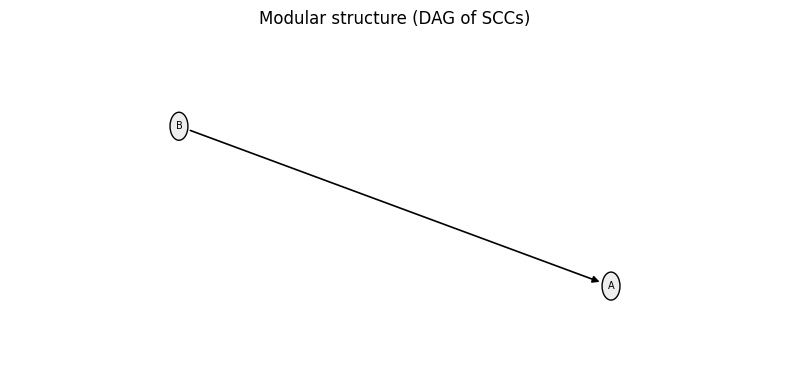
\includegraphics[keepaspectratio]{figures/tutorial06_boolean_networks_fig3.png}}

\begin{lstlisting}
cn.F:
  F[0] = BooleanFunction(name='A', f=[1, 0])
  F[1] = BooleanFunction(name='B', f=[1, 1])
cn.constants: {'C': 0}
\end{lstlisting}

Setting \(C = 0\) removes \(C\) from the reduced network \texttt{cn} (it
becomes a constant). Moreover, since \(B = \neg C\), we get \(B = 1\)
always, while the update rule for \(A\) is not changed.

\subsubsection{Edge controls}\label{edge-controls}

Similarly, we can implement edge controls. Edge control removes the
influence of a source node on a target node by fixing the source to a
specified value within the target's update function. The resulting
function is then simplified, and the corresponding edge is removed. As
an example, we consider a more connected Boolean network with different
types of update rules.

\begin{lstlisting}
string = """
A = B and C
B = A or C
C = A and not B
"""
bn = bf.BooleanNetwork.from_string(string, separator="=")
print("bn.I:", bn.I)
print("bn.F:")
for i, f in enumerate(bn.F):
    print(f"  F[{i}] = {f!r}")
print()

cn = bn.get_network_with_edge_controls(control_targets=[0],
                                       control_sources=[1],
                                       values_edge_controls=[0])
print("cn.I:", cn.I)
print("cn.F:")
for i, f in enumerate(cn.F):
    print(f"  F[{i}] = {f!r}")
\end{lstlisting}

\begin{lstlisting}
bn.I: [array([1, 2]), array([0, 2]), array([0, 1])]
bn.F:
  F[0] = BooleanFunction(name='A', f=[0, 0, 0, 1])
  F[1] = BooleanFunction(name='B', f=[0, 1, 1, 1])
  F[2] = BooleanFunction(name='C', f=[0, 0, 1, 0])

cn.I: [array([2]), array([0, 2]), array([0, 1])]
cn.F:
  F[0] = BooleanFunction(name='A', f=[0, 0])
  F[1] = BooleanFunction(name='B', f=[0, 1, 1, 1])
  F[2] = BooleanFunction(name='C', f=[0, 0, 1, 0])
\end{lstlisting}

By setting \(B=0\) in the regulation of \(A\), we remove \(B\)'s
influence on \(A\). Moreover, since \(A = B \wedge C\), we now have
\(A=0\) always.

\subsection{Outlook}\label{outlook}

In the remaining tutorials, we build on this foundation to study the
dynamical behavior of Boolean networks, including attractors, basins of
attraction, and stability under perturbations.

\section{Dynamics of Boolean
Networks}\label{dynamics-of-boolean-networks}

In this tutorial, we study the \emph{dynamics} of Boolean networks.
Building on the construction and structural analysis from previous
tutorials, we now focus on characterizing the long-term behavior of
Boolean networks.

\subsection{What you will learn}\label{what-you-will-learn-6}

You will learn how to:

\begin{itemize}
\tightlist
\item
  simulate Boolean network dynamics under different updating schemes,
\item
  compute and classify attractors,
\item
  analyze basins of attraction,
\item
  relate network structure to dynamical behavior.
\end{itemize}

\subsection{Setup}\label{setup-6}

\begin{lstlisting}
import boolforge as bf
import numpy as np
import pandas as pd
import matplotlib.pyplot as plt
\end{lstlisting}

\subsection{State space of a Boolean
network}\label{state-space-of-a-boolean-network}

A Boolean network with \(N\) nodes defines a dynamical system on the
discrete state space \(\{0,1\}^N\).

Each state is a binary vector

\[
\mathbf{x} = (x_0, \ldots, x_{N-1}) \in \{0,1\}^N,
\]

where \(x_i\) denotes the state of node \(i\).

We use a small Boolean network as a running example.

\begin{lstlisting}
string = """
x = y
y = x OR z
z = y
"""

bn = bf.BooleanNetwork.from_string(string, separator="=")

print("Variables:", bn.variables)
print("N:", bn.N)
print("bn.I:", bn.I)
print("bn.F:")
for i, f in enumerate(bn.F):
    print(f"  F[{i}] = {f!r}")
\end{lstlisting}

\begin{lstlisting}
Variables: ['x' 'y' 'z']
N: 3
bn.I: [array([1]), array([0, 2]), array([1])]
bn.F:
  F[0] = BooleanFunction(name='x', f=[0, 1])
  F[1] = BooleanFunction(name='y', f=[0, 1, 1, 1])
  F[2] = BooleanFunction(name='z', f=[0, 1])
\end{lstlisting}

All state vectors follow the variable order given by
\texttt{bn.variables}. For small networks, we can enumerate all \(2^N\)
states explicitly.

\begin{lstlisting}
all_states = bf.get_left_side_of_truth_table(bn.N)
print(pd.DataFrame(all_states, columns=bn.variables).to_string())
\end{lstlisting}

\begin{lstlisting}
   x  y  z
0  0  0  0
1  0  0  1
2  0  1  0
3  0  1  1
4  1  0  0
5  1  0  1
6  1  1  0
7  1  1  1
\end{lstlisting}

\subsection{Dynamics of synchronous Boolean
networks}\label{dynamics-of-synchronous-boolean-networks}

Under \emph{synchronous updating}, all nodes are updated simultaneously,
defining a deterministic update map

\[
\mathbf{x}(t+1) = F(\mathbf{x}(t)).
\]

\subsubsection{Exact computation}\label{exact-computation}

The update map \(F\) can be evaluated directly for any state vector. In
BoolForge, this is implemented by the method
\texttt{update\_network\_synchronously}. For convenience, Boolean
networks are callable, so that \texttt{bn(state)} evaluates the update
map and is equivalent to
\texttt{bn.update\_network\_synchronously(state)}.

\begin{lstlisting}
for state in all_states:
    print(state, "-->", bn(state))
\end{lstlisting}

\begin{lstlisting}
[0 0 0] --> [0 0 0]
[0 0 1] --> [0 1 0]
[0 1 0] --> [1 0 1]
[0 1 1] --> [1 1 1]
[1 0 0] --> [0 1 0]
[1 0 1] --> [0 1 0]
[1 1 0] --> [1 1 1]
[1 1 1] --> [1 1 1]
\end{lstlisting}

This output matches the synchronous truth table representation:

\begin{lstlisting}
print(bn.to_truth_table().to_string())
\end{lstlisting}

\begin{lstlisting}
   x(t)  y(t)  z(t)  x(t+1)  y(t+1)  z(t+1)
0     0     0     0       0       0       0
1     0     0     1       0       1       0
2     0     1     0       1       0       1
3     0     1     1       1       1       1
4     1     0     0       0       1       0
5     1     0     1       0       1       0
6     1     1     0       1       1       1
7     1     1     1       1       1       1
\end{lstlisting}

Each state has exactly one successor, so the dynamics consist of
transient trajectories leading into \emph{attractors} (steady states or
cycles).

In this example, the network has:

\begin{itemize}
\tightlist
\item
  two steady states: \((0,0,0)\) and \((1,1,1)\),
\item
  one cyclic attractor of length 2: \((0,1,0) \leftrightarrow (1,0,1)\).
\end{itemize}

\subsubsection{Exhaustive attractor
computation}\label{exhaustive-attractor-computation}

BoolForge contains a dedicated method to identify all attractors of a
network under synchronous update.

\begin{lstlisting}
dict_dynamics = bn.get_attractors_synchronous_exact()
\end{lstlisting}

The returned dictionary contains:

\begin{itemize}
\tightlist
\item
  \texttt{STG}: the synchronous state transition graph,
\item
  \texttt{NumberOfAttractors},
\item
  \texttt{Attractors},
\item
  \texttt{AttractorID},
\item
  \texttt{BasinSizes}.
\end{itemize}

For computational reasons, binary states in \(\{0,1\}^N\) are identified
by their decimal representation. The state transition graph can be
decoded as follows:

\begin{lstlisting}
for state in range(2   bn.N):
    next_state = dict_dynamics["STG"][state]
    print(
        state,
        "=",
        bf.dec2bin(state, bn.N),
        "-->",
        next_state,
        "=",
        bf.dec2bin(next_state, bn.N),
    )
\end{lstlisting}

\begin{lstlisting}
0 = [0, 0, 0] --> 0 = [0, 0, 0]
1 = [0, 0, 1] --> 2 = [0, 1, 0]
2 = [0, 1, 0] --> 5 = [1, 0, 1]
3 = [0, 1, 1] --> 7 = [1, 1, 1]
4 = [1, 0, 0] --> 2 = [0, 1, 0]
5 = [1, 0, 1] --> 2 = [0, 1, 0]
6 = [1, 1, 0] --> 7 = [1, 1, 1]
7 = [1, 1, 1] --> 7 = [1, 1, 1]
\end{lstlisting}

After repeated updates, the system settles into periodic behavior. That
is, irrespective of the initial state, an attractor is reached. The list
of all attractors (in decimal representation) can be displayed.

\begin{lstlisting}
print(dict_dynamics['Attractors'])
\end{lstlisting}

\begin{lstlisting}
[[0], [2, 5], [7]]
\end{lstlisting}

Attractors can be printed in binary representation:

\begin{lstlisting}
for attractor in dict_dynamics["Attractors"]:
    print(f"Attractor of length {len(attractor)}:")
    for state in attractor:
        print(state, bf.dec2bin(state, bn.N))
    print()
\end{lstlisting}

\begin{lstlisting}
Attractor of length 1:
0 [0, 0, 0]

Attractor of length 2:
2 [0, 1, 0]
5 [1, 0, 1]

Attractor of length 1:
7 [1, 1, 1]
\end{lstlisting}

The information which state transitions to which attractor is stored in
a dictionary. Here, the indices correspond to the list of attractors in
\texttt{dict\_dynamics{[}\textquotesingle{}Attractors\textquotesingle{}{]}}.

\begin{lstlisting}
for state_dec,attr_id in enumerate(dict_dynamics['AttractorID']):
    print(state_dec,'--> attractor',attr_id,
          'which is',dict_dynamics['Attractors'][attr_id])
\end{lstlisting}

\begin{lstlisting}
0 --> attractor 0 which is [0]
1 --> attractor 1 which is [2, 5]
2 --> attractor 1 which is [2, 5]
3 --> attractor 2 which is [7]
4 --> attractor 1 which is [2, 5]
5 --> attractor 1 which is [2, 5]
6 --> attractor 2 which is [7]
7 --> attractor 2 which is [7]
\end{lstlisting}

Finally, the basin size of each attractor is determined by the number of
states that eventually transition to an attractor. By definition, the
sum of all basin sizes is always \(2^N\). To simplify the comparison of
the basin size distribution for networks of different size,
\texttt{BoolForge} normalizes the basin sizes by default.

\begin{lstlisting}
print(dict_dynamics['BasinSizes'])
\end{lstlisting}

\begin{lstlisting}
[0.125 0.5   0.375]
\end{lstlisting}

From the previous two outputs, we see that there is no state (other than
000) that eventually transitions to 000. Half the states transition to
the 2-cycle, while 3 out of 8 states transition to the attractor 111.

\subsubsection{Monte Carlo simulation}\label{monte-carlo-simulation}

For larger networks, exhaustive enumeration is infeasible. Monte Carlo
simulation approximates the attractor landscape.

\begin{lstlisting}
dict_dynamics = bn.get_attractors_synchronous(n_simulations=1000)
print('Discovered attractors:',dict_dynamics['Attractors'])
print('Basin size approximation:',dict_dynamics['BasinSizesApproximation'])
\end{lstlisting}

\begin{lstlisting}
Discovered attractors: [[7], [5, 2], [0]]
Basin size approximation: [0.373 0.514 0.113]
\end{lstlisting}

The simulation returns additional information:

\begin{itemize}
\tightlist
\item
  sampled initial states,
\item
  the number of timeouts (trajectories not reaching an attractor before
  timeout).
\end{itemize}

\begin{lstlisting}
for key in dict_dynamics:
    print(key)
\end{lstlisting}

\begin{lstlisting}
Attractors
NumberOfAttractorsLowerBound
BasinSizesApproximation
AttractorID
InitialSamplePoints
STG
NumberOfTimeouts
\end{lstlisting}

In the absence of timeouts: If an attractor has relative basin size
\(q\), the probability that it is found from \(m\) random
initializations is \(1 - (1-q)^m\).

\begin{lstlisting}
qs = [0.0001, 0.001, 0.01, 0.1]
ms = np.logspace(0, 4, 1000)

fig, ax = plt.subplots()
for q in qs:
    ax.semilogx(ms, 1 - (1 - q)   ms, label=str(q))

ax.legend(title=r"$q$", frameon=False)
ax.set_xlabel("number of initial states ($m$)")
ax.set_ylabel("probability attractor of basin size q is found")
plt.show()
\end{lstlisting}

\pandocbounded{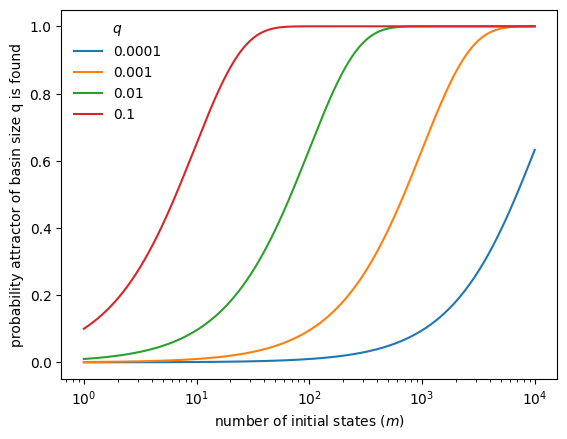
\includegraphics[keepaspectratio]{figures/tutorial07_network_dynamics_fig0.png}}

\subsection{Dynamics of asynchronous Boolean
networks}\label{dynamics-of-asynchronous-boolean-networks}

Synchronous updating is computationally convenient but biologically
unrealistic. Asynchronous updating assumes that only one node changes at
a time.

\subsubsection{Steady states under general asynchronous
update}\label{steady-states-under-general-asynchronous-update}

BoolForge can compute steady states under \emph{general asynchronous
updating}, where at each step only a single node updates according to
its Boolean rule.

\begin{lstlisting}
dict_dynamics = bn.get_steady_states_asynchronous_exact()
print('Discovered steady states:',dict_dynamics['SteadyStates'])
print('Number of steady states (lower bound):',dict_dynamics['NumberOfSteadyStates'])
\end{lstlisting}

\begin{lstlisting}
Discovered steady states: [0, 7]
Number of steady states (lower bound): 2
\end{lstlisting}

The result reveals the same two steady states as in the synchronous
case. However, the limit cycle observed under synchronous updating
disappears under asynchronous dynamics.

In addition, BoolForge returns the \emph{full asynchronous state
transition graph}.

\begin{lstlisting}
for state, successors in dict_dynamics["STGAsynchronous"].items():
    print(state,'-->',successors)
\end{lstlisting}

\begin{lstlisting}
0 --> {0: 1.0}
1 --> {1: 0.3333333333333333, 3: 0.3333333333333333, 0: 0.3333333333333333}
2 --> {6: 0.3333333333333333, 0: 0.3333333333333333, 3: 0.3333333333333333}
3 --> {7: 0.3333333333333333, 3: 0.6666666666666666}
4 --> {0: 0.3333333333333333, 6: 0.3333333333333333, 4: 0.3333333333333333}
5 --> {1: 0.3333333333333333, 7: 0.3333333333333333, 4: 0.3333333333333333}
6 --> {6: 0.6666666666666666, 7: 0.3333333333333333}
7 --> {7: 1.0}
\end{lstlisting}

The state transition graph describes for each state the possible next
states that the system may transition to, in addition to the transition
probabilities. This graph can be interpreted as a \emph{sparse
transition matrix} of a Markov chain. Each directed edge corresponds to
a possible single-node update.

By repeatedly composing this transition matrix with itself
(equivalently, raising it to higher powers), BoolForge computes the
\emph{absorption probabilities}, i.e., the probability that a trajectory
starting from any state eventually reaches each steady state.

\begin{lstlisting}
print(dict_dynamics['FinalTransitionProbabilities'])
\end{lstlisting}

\begin{lstlisting}
[[1.         0.        ]
 [0.5        0.5       ]
 [0.33333333 0.66666667]
 [0.         1.        ]
 [0.5        0.5       ]
 [0.33333333 0.66666667]
 [0.         1.        ]
 [0.         1.        ]]
\end{lstlisting}

The size of each basin of attraction is the (column-wise) average of
these probabilities.

\begin{lstlisting}
assert np.all(dict_dynamics['BasinSizes'] == 
              np.mean(dict_dynamics['FinalTransitionProbabilities'],0))
print('Basin sizes:',dict_dynamics['BasinSizes'])
\end{lstlisting}

\begin{lstlisting}
Basin sizes: [0.33333333 0.66666667]
\end{lstlisting}

Note that \texttt{BoolForge} currently does not detect complex cyclic
attractors under asynchronous update; for this task, specialized tools
such as \href{https://github.com/jcrozum/pystablemotifs}{pystablemotifs}
are recommended \citep{rozum2022pystablemotifs}.

In fact, some of BoolForge's asynchronous update methods fail when the
network contains no steady state.

\subsubsection{Monte Carlo
approximation}\label{monte-carlo-approximation}

As in the synchronous case, \texttt{BoolForge} also contains a Monte
Carlo routine for sampling asynchronous dynamics.

The simulation provides:

\begin{itemize}
\tightlist
\item
  a lower bound on the number of steady states,
\item
  approximate basin size distributions,
\end{itemize}

\begin{lstlisting}
dict_dynamics = bn.get_steady_states_asynchronous(n_simulations=500)
print('Discovered steady states:', dict_dynamics['SteadyStates'])
print('Number of steady states (lower bound):',dict_dynamics['NumberOfSteadyStatesLowerBound'])
print('Basin size approximation:',dict_dynamics['BasinSizesApproximation'])
\end{lstlisting}

\begin{lstlisting}
Discovered steady states: [7, 0, 11]
Number of steady states (lower bound): 3
Basin size approximation: [0.556 0.366 0.078]
\end{lstlisting}

\subsubsection{Sampling from a fixed initial
condition}\label{sampling-from-a-fixed-initial-condition}

In biological Boolean network models, a specific state
\(\mathbf x \in \{0,1\}^N\) is frequently considered the initial state,
e.g., corresponding to the G0 phase of the cell cylce. To enable
exploration of the stochastic trajectories from a specific state,
BoolForge contains the following method.

\begin{lstlisting}
dict_dynamics = bn.get_steady_states_asynchronous_given_one_initial_condition(
    initial_condition=[0, 0, 1], n_simulations=500
)
print('Discovered steady states:', dict_dynamics['SteadyStates'])
print('Number of steady states (lower bound):',dict_dynamics['NumberOfSteadyStatesLowerBound'])
print('Basin size approximation:',dict_dynamics['BasinSizesApproximation'])
\end{lstlisting}

\begin{lstlisting}
Discovered steady states: [0, 7, 2]
Number of steady states (lower bound): 3
Basin size approximation: [0.522 0.212 0.266]
\end{lstlisting}

Note the equivalent analysis under synchronous update is trivial because
the dynamics are deterministic and the long-term behavior when starting
in a specific initial condition can be found by

\begin{lstlisting}
dict_dynamics = bn.get_attractors_synchronous(n_simulations=1,
                                              initial_sample_points=[[0,0,1]],
                                              initial_sample_points_are_vectors=True)
dict_dynamics
\end{lstlisting}

\begin{lstlisting}
{'Attractors': [[2, 5]],
 'NumberOfAttractorsLowerBound': 1,
 'BasinSizesApproximation': array([1.]),
 'AttractorID': {2: 0, 5: 0},
 'InitialSamplePoints': [[0, 0, 1]],
 'STG': {1: 2},
 'NumberOfTimeouts': 0}
\end{lstlisting}

\subsection{Summary}\label{summary-5}

In this tutorial you learned how to:

\begin{itemize}
\tightlist
\item
  simulate Boolean network dynamics,
\item
  compute synchronous attractors exactly and approximately,
\item
  analyze basin sizes,
\item
  compute steady states under asynchronous updating.
\end{itemize}

This concludes the function- and network-level analysis. Subsequent
tutorials focus on analyzing stability to perturbations, control
analysis, and ensemble experiments.

\section{Perturbation and sensitivity analysis of Boolean
networks}\label{perturbation-and-sensitivity-analysis-of-boolean-networks}

In this tutorial, we study how Boolean networks respond to
perturbations. Rather than implementing perturbations manually, we
leverage BoolForge's built-in robustness and sensitivity measures.

\subsection{What you will learn}\label{what-you-will-learn-7}

You will learn how to:

\begin{itemize}
\tightlist
\item
  quantify robustness and fragility of Boolean networks under
  synchronous update,
\item
  interpret basin-level and attractor-level robustness measures,
\item
  perform exact and approximate robustness computations, and
\item
  compute Derrida values as a measure of dynamical sensitivity.
\end{itemize}

Together, these tools allow us to assess dynamical stability and
resilience of Boolean network models in a principled and computationally
efficient way.

\subsection{Setup}\label{setup-7}

\begin{lstlisting}
import boolforge as bf
import pandas as pd
\end{lstlisting}

We reuse the small Boolean network from the previous tutorial as a
running example.

\begin{lstlisting}
string = """
x = y
y = x OR z
z = y
"""

bn = bf.BooleanNetwork.from_string(string, separator="=")

print("Variables:", bn.variables)
print("Number of nodes:", bn.N)
\end{lstlisting}

\begin{lstlisting}
Variables: ['x' 'y' 'z']
Number of nodes: 3
\end{lstlisting}

\subsection{Exact attractors and robustness
measures}\label{exact-attractors-and-robustness-measures}

BoolForge provides a single method that computes:

\begin{itemize}
\tightlist
\item
  all attractors,
\item
  basin sizes,
\item
  overall network coherence and fragility,
\item
  basin-level coherence and fragility, and
\item
  attractor-level coherence and fragility.
\end{itemize}

These quantities are defined via systematic single-bit perturbations in
the Boolean hypercube and can be computed \emph{exactly} for small
networks.

\begin{lstlisting}
results_exact = bn.get_attractors_and_robustness_synchronous_exact()
for key in results_exact.keys():
    print(key)
\end{lstlisting}

\begin{lstlisting}
Attractors
NumberOfAttractors
BasinSizes
AttractorID
Coherence
Fragility
BasinCoherences
BasinFragilities
AttractorCoherences
AttractorFragilities
\end{lstlisting}

For convenience, information about the dynamics (attractors, basin
sizes, etc), described in detail in the previous tutorial, is also
returned by this method.

\begin{lstlisting}
print("Number of attractors:", results_exact["NumberOfAttractors"])
print("Attractors (decimal states):", results_exact["Attractors"])
print("Eventual attractor of each state:", results_exact["AttractorID"])

print("Basin sizes:", results_exact["BasinSizes"])
\end{lstlisting}

\begin{lstlisting}
Number of attractors: 3
Attractors (decimal states): [[0], [2, 5], [7]]
Eventual attractor of each state: [0 1 1 2 1 1 2 2]
Basin sizes: [0.125 0.5   0.375]
\end{lstlisting}

\subsection{Network-, basin- and attractor-level
robustness}\label{network--basin--and-attractor-level-robustness}

Robustness can be resolved at different structural levels. Network-level
metrics report the average robustness of any network state when
subjected to perturbation.

\begin{lstlisting}
print("Overall coherence:", results_exact["Coherence"])
print("Overall fragility:", results_exact["Fragility"])
\end{lstlisting}

\begin{lstlisting}
Overall coherence: 0.3333333333333333
Overall fragility: 0.3333333333333333
\end{lstlisting}

The same robustness metrics, coherence and fragility, can also be
averaged across a smaller set of states, e.g., all states in one basin
of attraction (see \citet{bavisetty2025upper}), or an even smaller set
of states, e.g., all states that form an attractor (see
\citet{bavisetty2025attractors}).

\begin{lstlisting}
df_basins = pd.DataFrame({
    "BasinSizes": results_exact["BasinSizes"],
    "BasinCoherences": results_exact["BasinCoherences"],
    "BasinFragilities": results_exact["BasinFragilities"],
})

df_attractors = pd.DataFrame({
    "AttractorCoherences": results_exact["AttractorCoherences"],
    "AttractorFragilities": results_exact["AttractorFragilities"],
})

print("Basin-level robustness:")
print(df_basins)

print("Attractor-level robustness:")
print(df_attractors)
\end{lstlisting}

\begin{lstlisting}
Basin-level robustness:
   BasinSizes  BasinCoherences  BasinFragilities
0       0.125         0.000000          0.500000
1       0.500         0.333333          0.333333
2       0.375         0.444444          0.277778
Attractor-level robustness:
   AttractorCoherences  AttractorFragilities
0             0.000000              0.500000
1             0.333333              0.333333
2             0.666667              0.166667
\end{lstlisting}

Interpretation:

\begin{itemize}
\tightlist
\item
  \emph{Coherence} measures the fraction of single-bit perturbations
  that do \emph{not} change the final attractor \citep{willadsenwiles}.
\item
  \emph{Fragility} measures how much the attractor state changes
  \citep{park2023models}.
\end{itemize}

The robustness metrics considered thus far describe how a single
perturbation affects the network dynamics in the long-term, i.e., at the
attractor. These metrics are very meaningful biologically because
attractors typically correspond to cell types of phenotypes.

It turns out that attractors in biological networks are often less
stable than their basins, a phenomenon explored in detail in Tutorial
10.

\subsection{Approximate robustness for larger
networks}\label{approximate-robustness-for-larger-networks}

For larger networks, exact enumeration of all \(2^N\) states is
infeasible. BoolForge therefore provides a Monte Carlo approximation
that samples random initial conditions and perturbations.

\begin{lstlisting}
results_approx = bn.get_attractors_and_robustness_synchronous(n_simulations=500)

print("Number of attractors (lower bound):", results_approx["NumberOfAttractorsLowerBound"])
print("Approximate coherence:", results_approx["CoherenceApproximation"])
print("Approximate fragility:", results_approx["FragilityApproximation"])
\end{lstlisting}

\begin{lstlisting}
Number of attractors (lower bound): 3
Approximate coherence: 0.306
Approximate fragility: 0.347
\end{lstlisting}

Even when only using 500 random initial states, the approximate values
closely match the exact ones. For larger networks, these approximations
are often the only feasible option.

\subsection{Derrida value: dynamical
sensitivity}\label{derrida-value-dynamical-sensitivity}

An older and very popular robustness metric, the Derrida value, measures
how perturbations \emph{propagate} after one synchronous update
\citep{derrida1986random}. It is defined as the expected Hamming
distance between updated states that initially differed in exactly one
bit.

BoolForge includes routines for the exact calculation and estimation of
Derrida values. For networks with low degree, the exact calculation is
strongly preferable. It is faster and more accurate.

\begin{lstlisting}
derrida_exact = bn.get_derrida_value(exact=True)
derrida_approx = bn.get_derrida_value(n_simulations=2000)

print("Exact Derrida value:", derrida_exact)
print("Approximate Derrida value:", derrida_approx)
\end{lstlisting}

\begin{lstlisting}
Exact Derrida value: 1.0
Approximate Derrida value: 1.0
\end{lstlisting}

Interpretation:

\begin{itemize}
\tightlist
\item
  Small Derrida values indicate ordered, stable dynamics.
\item
  Large Derrida values indicate sensitive or chaotic dynamics.
\end{itemize}

Derrida values are closely related to average sensitivity of the update
functions, and provide a complementary notion of robustness.

\subsection{Summary}\label{summary-6}

In this tutorial you learned how to:

\begin{itemize}
\tightlist
\item
  compute exact robustness measures for small Boolean networks,
\item
  interpret coherence and fragility at network, basin, and attractor
  levels,
\item
  approximate robustness measures for larger networks, and
\item
  assess dynamical sensitivity using the Derrida value.
\end{itemize}

In Tutorial 9, we will finally analyze biological Boolean network models
and design ensemble experiments.

\section{Random Boolean network
generation}\label{random-boolean-network-generation}

This tutorial demonstrates how to generate \emph{random Boolean networks
with controlled structural and functional properties} using BoolForge.
This ability enables ensemble studies, which are exemplified in the next
tutorial.

\subsection{What you will learn}\label{what-you-will-learn-8}

In this tutorial you will learn how to generate random Boolean networks
with

\begin{itemize}
\tightlist
\item
  prescribed structural properties (e.g., degree, degree distribution,
  strongly connected),
\item
  prescribed functional properties (e.g., canalization, bias),
\end{itemize}

It is strongly recommended to complete Tutorials 4 and 5 on random
function generation first.

\subsection{Setup}\label{setup-8}

\begin{lstlisting}
import boolforge as bf
import numpy as np
import matplotlib.pyplot as plt
\end{lstlisting}

\subsection{Generating random wiring
diagrams}\label{generating-random-wiring-diagrams}

The function \texttt{random\_network(N,\ n,\ *args)} generates a random
\(N\)-node Boolean network with degree parameter \texttt{n}. The
generation follows a two-step process:

\begin{itemize}
\tightlist
\item
  A random wiring diagram is created using
  \texttt{random\_wiring\_diagram(N,\ n,\ *args)}.
\item
  Random Boolean functions with prescribed properties are generated
  using \texttt{random\_function(n,\ *args)}, which was discussed in
  depth in Tutorials 4 and 5.
\end{itemize}

We first consider only the structural parameters that concern the
generation of the random wiring diagram. In the absence of optional
arguments, the in-degree distribution is assumed to be constant. That
is, each node in the network is regulated by \texttt{n} nodes.

\begin{lstlisting}
N = 5
n = 2

W = bf.random_wiring_diagram(N, n, rng=2)

W.plot();
\end{lstlisting}

\pandocbounded{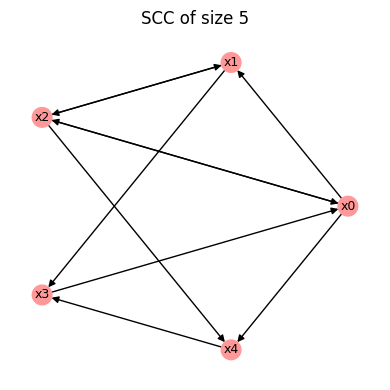
\includegraphics[keepaspectratio]{figures/tutorial09_random_Boolean_network_generation_fig1.png}}

The argument \texttt{rng} seeds the random number generator, ensuring
reproducible results.

The rest of this tutorial describes the various constraints / optional
arguments. Each optional argument restricts the family of networks from
which \texttt{random\_wiring\_diagram()} and \texttt{random\_network()}
samples.

\subsubsection{Allowing self-regulation}\label{allowing-self-regulation}

BoolForge selects the \texttt{n} regulators of each node uniformly at
random from the set of all other nodes. Thus, self-regulation is
disallowed by default. Setting \texttt{allow\_self\_loops=True} allows
nodes to regulate themselves.

\begin{lstlisting}
N = 5
n = 2

W = bf.random_wiring_diagram(N,n,allow_self_loops=True,rng = 2)

W.plot();
\end{lstlisting}

\pandocbounded{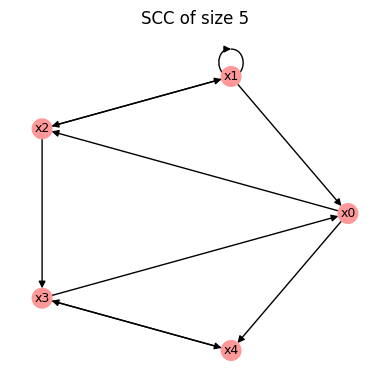
\includegraphics[keepaspectratio]{figures/tutorial09_random_Boolean_network_generation_fig2.png}}

\subsubsection{Poisson in-degree
distributions}\label{poisson-in-degree-distributions}

Classical random Boolean network theory (NK Kauffman models) assume a
fixed in-degree, the default in BoolForge. However, this is a strong
assumption since the in-degree in curated biological Boolean network
models often appears approximately Poisson distributed. BoolForge
provides the option to generate random wiring diagrams with Poisson
distributed in-degree, using the optional parameter
\texttt{indegree\_distribution}.

\begin{lstlisting}
N = 5
n = 2

W = bf.random_wiring_diagram(N,n,indegree_distribution='poisson',rng = 5)

W.plot();
\end{lstlisting}

\pandocbounded{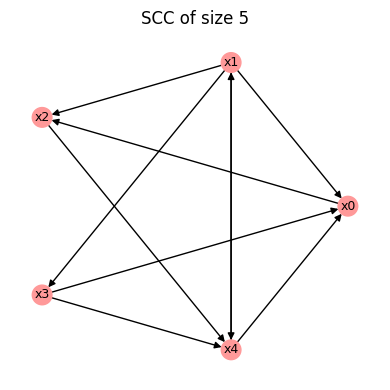
\includegraphics[keepaspectratio]{figures/tutorial09_random_Boolean_network_generation_fig3.png}}

We see that some nodes (\(x_1\) and \(x_3\)) are only regulated by one
node, while others (\(x_0\) and \(x_4\)) possess three regulators each.

When using a Poisson-distributed in-degree, the in-degree of every node
is always at least 1. This avoids the artificial creation of identity
nodes (with in-degree 0).

\subsubsection{Avoiding output nodes}\label{avoiding-output-nodes}

In general, it is possible that some nodes in a generated Boolean
network will not regulate other nodes. By setting
\texttt{min\_out\_degree\_one=True}, we can force every node to regulate
at least one node. That is, output nodes can be disallowed.

\subsubsection{Strong connectedness}\label{strong-connectedness}

The wiring diagram of the generated Boolean network may or may not be
strongly connected. Setting \texttt{strongly\_connected=True} (default
False) forces strong connectedness. Uniform sampling among strongly
connected networks cannot be achieved by a simple construction method.
BoolForge therefore generates candidate networks and rejects them until
a strongly connected network is obtained.

Careful: When the number of nodes \texttt{N} is large and the degree
\texttt{n} is small, this may take a long time. The number of
unsuccessful attempts before raising an error is controlled by the
optional parameter \texttt{max\_strong\_connectivity\_attempts}.

\subsubsection{Fixed wiring diagrams}\label{fixed-wiring-diagrams}

All optional parameters discussed thus far describe properties of the
wiring diagram. Instead of generating a new wiring diagram, an existing
one (e.g., from a curated biological network model) can be passed
directly to \texttt{random\_network}.

In that case, \texttt{random\_network(I,\ *args)} does not require
\texttt{N} and \texttt{n}, because these quantities are inferred from
the wiring diagram, provided via optional parameter \texttt{I}. As
described in detail in Tutorial 6, \texttt{I} can be either a
\texttt{WiringDiagram} object or a list of lists describing the
regulators of each node.

For example, using the previously generated wiring diagram, we can write

\begin{lstlisting}
bn = bf.random_network(I=W)
\end{lstlisting}

This feature allows multiple Boolean networks with different update
functions to be generated on the same wiring diagram.

\subsection{Specifying functional
constraints}\label{specifying-functional-constraints}

Once the wiring diagram is generated, the number of nodes \texttt{N} and
the in-degree of each node are determined. In step 2,
\texttt{random\_network} now repeatedly calls \texttt{random\_function}
to generate the random Boolean functions. The optional parameters
regulating the functional constraints are practically identical to the
ones discussed in depth in Tutorial 4, with one important distinction:
Most parameters can be sequences of length \texttt{N}, in order to
specify distinct functional behavior for the different nodes.

In the following, we summarize the key concepts.

\subsubsection{Parity functions}\label{parity-functions-1}

If \texttt{parity=True} (default False), parity functions (also known as
linear functions) are chosen for all nodes, yielding a linear Boolean
network (see \citet{chandrasekhar2023stability}). Note that for any
degree \texttt{n}, there are only two parity functions.

\subsubsection{Canalizing functions}\label{canalizing-functions}

If a specific \texttt{layer\_structure} is provided, all functions
possess at least these canalizing layers.

\begin{lstlisting}
bn = bf.random_network(N=4,n=3,layer_structure=[1],rng = 2)
for f in bn.F:
    print(f,f.get_layer_structure()['LayerStructure'])
\end{lstlisting}

\begin{lstlisting}
[0 1 1 0 0 0 0 0] [1]
[0 0 1 1 0 1 1 1] [1, 2]
[0 0 0 0 0 0 0 1] [3]
[1 1 1 0 1 1 1 1] [3]
\end{lstlisting}

As we see, it is however possible for some functions to randomly possess
more canalizing variables in a larger and/or more layers. To ensure
\texttt{layer\_structure} is interpreted as exact layer structure, set
\texttt{exact\_depth=True}.

\begin{lstlisting}
bn = bf.random_network(N=4,n=3,layer_structure=[1],exact_depth=True,rng = 2)
for f in bn.F:
    print(f,f.get_layer_structure()['LayerStructure'])
\end{lstlisting}

\begin{lstlisting}
[0 1 1 0 0 0 0 0] [1]
[1 0 1 1 0 1 1 1] [1]
[1 1 0 1 0 1 1 1] [1]
[0 1 1 0 1 1 1 1] [1]
\end{lstlisting}

Rather than specifying the exact layer structure, we can also describe
the desired \emph{canalizing depth} (i.e., the number of conditionally
canalizing variables) via \texttt{depth}. As before, the optional
argument \texttt{exact\_depth} (default False) determines if
\texttt{depth} is interpreted as exact canalizing depth, or as minimum
canalizing depth.

\begin{lstlisting}
#Boolean network whose rules all have minimal canalizing depth 1
bn1 = bf.random_network(N=4,n=3,depth=1,exact_depth=False,rng = 2)
for f in bn1.F:
    print(f.get_canalizing_depth(),f) 
print()    

#Boolean network whose rules all have exact canalizing depth 1
bn2 = bf.random_network(N=4,n=3,depth=1,exact_depth=True,rng = 2)
for f in bn2.F:
    print(f.get_canalizing_depth(),f) 
\end{lstlisting}

\begin{lstlisting}
1 [0 1 1 0 0 0 0 0]
3 [0 0 0 0 0 0 1 0]
3 [1 1 0 0 1 1 1 0]
3 [0 1 1 1 0 0 0 0]

1 [0 1 1 0 0 0 0 0]
1 [1 0 0 0 0 0 1 0]
1 [1 1 0 1 0 1 1 1]
1 [0 0 1 0 1 0 0 0]
\end{lstlisting}

Most optional parameters (e.g., \texttt{n}, \texttt{depth},
\texttt{layer\_structure}, \texttt{bias}, \texttt{absolute\_bias}) can
also be specified as sequences of length \texttt{N}. In that case, each
entry applies to one node in the network, allowing different functional
constraints for different nodes.

\begin{lstlisting}
bn = bf.random_network(
    N=4,
    n=[3,3,2,2],
    depth=[3,1,2,0],
    exact_depth=True,
    rng=2
)

for f in bn.F:
    print(f.get_canalizing_depth(),f) 
\end{lstlisting}

\begin{lstlisting}
3 [1 1 1 1 0 1 1 1]
1 [1 1 0 1 0 1 1 1]
2 [1 1 0 1]
0 [0 1 1 0]
\end{lstlisting}

\subsubsection{Biased functions}\label{biased-functions}

When \texttt{parity=False} and all canalization parameters are also at
their default values, \texttt{random\_network} generates each update
function with a specified \emph{bias}, i.e.

\begin{itemize}
\tightlist
\item
  probability of output 1: \texttt{bias}
\item
  probability of output 0: \texttt{1-bias}
\end{itemize}

The unbiased case (\texttt{bias=0.5}) is the default. Instead of the
bias, users can also specify the absolute bias to generate functions
with a bimodal Hamming weight distribution. For BoolForge to use the
parameter provided via \texttt{absolute\_bias},
\texttt{use\_absolute\_bias=True} is required. The default is
\texttt{use\_absolute\_bias=False}, i.e., by default \texttt{bias} is
used, resulting in a unimodal Hamming weight distribution.

\begin{lstlisting}
N = 1000 #network size
n = 4   #constant in-degree

bn1 = bf.random_network(N=N,n=n,bias=0.75)
bn2 = bf.random_network(N=N,n=n,absolute_bias=0.5,use_absolute_bias=True)
bn3 = bf.random_network(N=N,n=n,absolute_bias=0.5)
bns = [bn1,bn2,bn3]

labels = ["bias = 0.75", "absolute bias = 0.5", "bias = 0.5 (balanced)"]
possible_hamming_weights = np.arange(2 n + 1)
width = 0.3

fig, ax = plt.subplots()
for i,bn in enumerate(bns):
    count = np.zeros(2 n + 1)
    for f in bn.F:
        count[f.hamming_weight] += 1
    ax.bar(possible_hamming_weights - width + i * width, 
           count / N, 
           width=width, label=labels[i])

ax.legend(frameon=False)
ax.set_xticks(possible_hamming_weights)
ax.set_xlabel("Hamming weight")
ax.set_ylabel("Proportion of update functions");
\end{lstlisting}

\pandocbounded{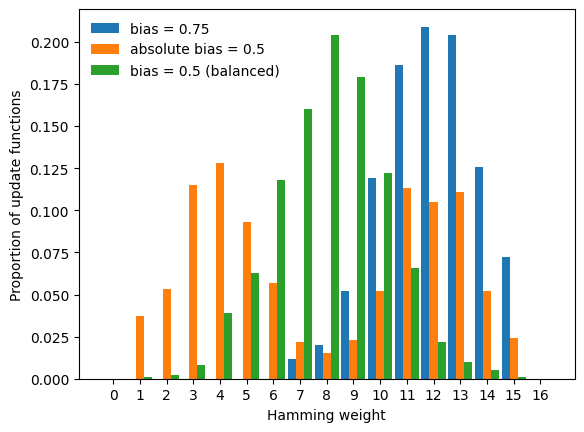
\includegraphics[keepaspectratio]{figures/tutorial09_random_Boolean_network_generation_fig0.png}}

\subsection{Summary}\label{summary-7}

In this tutorial you learned how to:

\begin{itemize}
\tightlist
\item
  generate random wiring diagrams with prescribed structural
  constraints,
\item
  generate, for each node in a wiring diagram, random update functions
  with prescribed functional constraints.
\end{itemize}

In the next tutorial, we will explore several situations, in which the
ability to generate large ensembles of controlled random Boolean
networks is very useful.

\section{Ensemble experiments with random Boolean
networks}\label{ensemble-experiments-with-random-boolean-networks}

This tutorial demonstrates how BoolForge's ability to generate
\emph{random Boolean networks with controlled structural and functional
properties} is essential for many types of studies. Specifically, it
enables:

\begin{enumerate}
\def\labelenumi{\arabic{enumi}.}
\item
  Null model comparisons:\\
  Are biological networks structurally or dynamically different from
  random networks?
\item
  Ensemble studies: How do structural properties such as degree or
  canalization affect network dynamics?
\end{enumerate}

\subsection{What you will learn}\label{what-you-will-learn-9}

In this tutorial you will learn how to generate random Boolean networks
with:

\begin{itemize}
\tightlist
\item
  specific structural properties (e.g., degree, degree distribution,
  strongly connected),
\item
  prescribed functional properties (e.g., canalization, bias),
\end{itemize}

It is strongly recommended to complete Tutorials 4 and 5 on random
function generation first.

\subsection{Setup}\label{setup-9}

\begin{lstlisting}
import boolforge as bf
import numpy as np
import matplotlib.pyplot as plt
\end{lstlisting}

\subsection{NK Kauffman networks}\label{nk-kauffman-networks}

One of the classical models of complex systems is the \emph{NK random
Boolean network} introduced by Stuart Kauffman.

In this model:

\begin{itemize}
\item
  The network contains N nodes.
\item
  Each node is regulated by k inputs.
\item
  Each update function is generated randomly with \emph{bias} \(p\),
  i.e.

  \begin{itemize}
  \tightlist
  \item
    probability of output 1: \texttt{p}
  \item
    probability of output 0: \texttt{1-p}
  \end{itemize}
\end{itemize}

A key theoretical result due to \citet{derrida1986random} predicts how a
single-node perturbation propagates in large random Boolean networks.
They showed that if two network states differ in one node, the expected
number of differences after one update step is \(2kp(1-p)\).

If this value is

\begin{itemize}
\tightlist
\item
  \(< 1\), then perturbations decrease on average (ordered regime)
\item
  \(> 1\), then perturbations increase on average (chaotic regime)
\item
  \(= 1\), then perturbations remain on average of equal size (critical
  boundary)
\end{itemize}

The expected number of propagated perturbations is called the
\emph{Derrida value}.

\begin{lstlisting}
N = 100          # network size
ks = range(1,5)  # constant in-degree
n_networks = 50  # ensemble size
p = 0.5          # bias p: probability of ones in truth table

derrida_values = []
for k in ks:
    derrida_values.append([])
    for _ in range(n_networks):
        bn = bf.random_network(N, k, bias = p, allow_degenerate_functions=True)
        derrida_values[-1].append( bn.get_derrida_value(exact=True) )

plt.boxplot(derrida_values, positions=list(ks))
plt.axhline(1, linestyle="--", color="gray", label="critical value")
plt.plot(ks, [2*k*p*(1-p) for k in ks], "o-", label=r"$2kp(1-p)$ (annealed theory)")
plt.xlabel("Constant in-degree k")
plt.ylabel("Derrida value")
plt.legend(frameon=False);
\end{lstlisting}

\pandocbounded{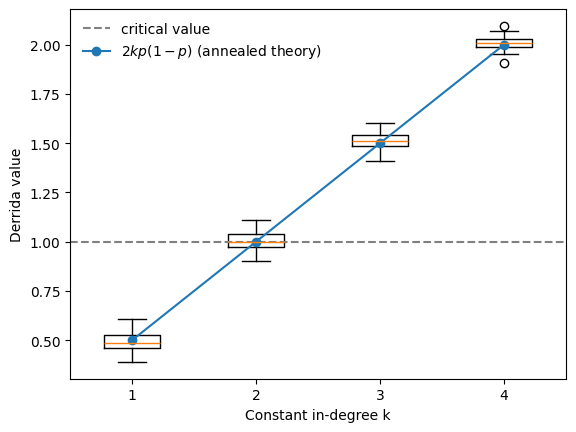
\includegraphics[keepaspectratio]{figures/tutorial10_ensemble_experiments_random_networks_fig0.png}}

The numerical results closely follow the theoretical prediction
\(2kp(1-p)\) derived under the \emph{annealed approximation}. The phase
transition occurs when the Derrida value crosses 1.

For unbiased Boolean functions (with bias \(p=0.5\)), the theory
predicts the critical connectivity \(k=2\), which we also observe in
this BoolForge ensemble experiment.

We encourage the reader to vary the bias \(p\) in the above example. As
the bias becomes more extreme, the Derrida value declines and networks
with higher connectivity exhibit critical dynamics.

\subsection{BoolForge philosophy: regulatory functions are
non-degenerate}\label{boolforge-philosophy-regulatory-functions-are-non-degenerate}

The classical NK model assumes that a Boolean function with \(k\) inputs
may \emph{not actually depend on all of them}. Such functions are called
\emph{degenerate}.

While this assumption is natural in statistical physics models
(e.g.~spin glasses), it is biologically questionable. In gene regulatory
networks, an input typically represents a \emph{specific regulatory
interaction}. If a transcription factor does not affect the gene, it
should not appear as an input in the first place. \emph{Therefore
BoolForge assumes non-degenerate Boolean functions by default.}

Degeneracy occurs frequently for small input sizes:

\begin{itemize}
\tightlist
\item
  \(k=1\): 2 out of 4 functions are degenerate (50\%)
\item
  \(k=2\): 6 out of 16 functions are degenerate
\item
  larger \(k\): degeneracy becomes increasingly rare
\end{itemize}

Disallowing degenerate functions therefore mainly affects sparse
networks, precisely the regime most biological networks operate in
(typical average in-degree \(\approx\) 2-3).

We now repeat the previous experiment, \emph{disallowing degenerate
functions}.

\begin{lstlisting}
derrida_values = []
for k in ks:
    derrida_values.append([])
    for _ in range(n_networks):
        bn = bf.random_network(N, k, bias = p, allow_degenerate_functions=False)
        derrida_values[-1].append( bn.get_derrida_value(exact=True) )

plt.boxplot(derrida_values, positions=list(ks))
plt.axhline(1, linestyle="--", color="gray", label="critical value")
plt.plot(ks, [2*k*p*(1-p) for k in ks], "o-", label=r"$2kp(1-p)$ (annealed theory)")
plt.xlabel("Constant in-degree k")
plt.ylabel("Derrida value")
plt.legend(frameon=False);
\end{lstlisting}

\pandocbounded{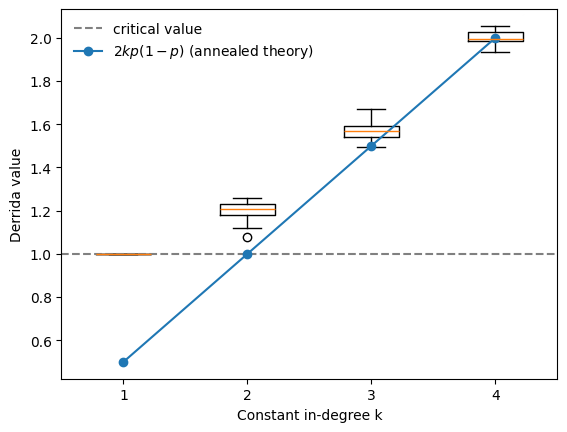
\includegraphics[keepaspectratio]{figures/tutorial10_ensemble_experiments_random_networks_fig1.png}}

The behavior changes substantially. For \emph{unbiased, non-degenerate
Boolean networks (with bias \(p=0.5\))} the phase transition occurs
already at \(k=1\), rather than \(k=2\), as predicted by the classical
NK theory.

This illustrates how biologically motivated modeling assumptions can
significantly affect the predicted dynamical regime of Boolean networks.

\subsection{Random networks with prescribed
canalization}\label{random-networks-with-prescribed-canalization}

A major advantage of BoolForge is its ability to generate Boolean
functions with \emph{controlled canalization properties}. This is
important because canalization is a common feature of biological
regulatory networks.

To display the impact of the canalizing layer structure, we generate
ensembles of Boolean networks of fixed size and fixed in-degree, which
are governed by nested canalizing functions of variable layer structure.

\begin{lstlisting}
N = 12           # network size
n = 5            # constant in-degree
n_networks = 100 # ensemble size

all_hamming = np.arange(1, 2   (n - 1), 2)
all_abs_bias = 2 * np.abs(all_hamming/2 n - 0.5)

number_attractors = []
number_steady_states = []
for i, w in enumerate(all_hamming):
    layer_structure = bf.hamming_weight_to_ncf_layer_structure(n, w)
    number_attractors.append([])
    number_steady_states.append([])
    for _ in range(n_networks):
        bn = bf.random_network(N, n, layer_structure=layer_structure)
        attr_info = bn.get_attractors_synchronous_exact()
        n_attractors = attr_info['NumberOfAttractors']
        number_attractors[-1].append( n_attractors )
        number_steady_states[-1].append( 
            sum([len(a)==1 for a in attr_info['Attractors']]) 
        )

fig,ax = plt.subplots()
mean, std = np.mean(number_attractors,1), np.std(number_attractors,1)
ax.plot(all_abs_bias, mean, 'rx:', label='attractors')
ax.fill_between(all_abs_bias, mean-std, mean+std, color='r', alpha = 0.2)
mean, std = np.mean(number_steady_states,1), np.std(number_steady_states,1)
ax.plot(all_abs_bias, mean, 'bo--', label='steady states')
ax.fill_between(all_abs_bias, mean-std, mean+std, color='b', alpha = 0.2)
ax.set_xlabel("Absolute bias")
ax.set_ylabel("Number")
ax.legend(frameon=False,loc='best');
\end{lstlisting}

\pandocbounded{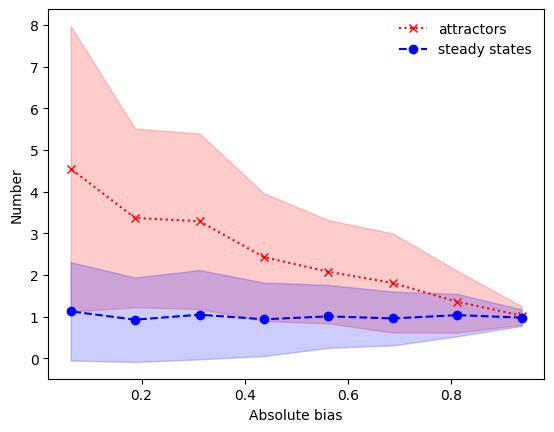
\includegraphics[keepaspectratio]{figures/tutorial10_ensemble_experiments_random_networks_fig2.png}}

This plot shows: The higher the absolute bias of the governing nested
canalizing functions, the more ordered the dynamics, characterized by
the presence of only a few network attractors, which are primarily
steady states.

\subsection{Summary and outlook}\label{summary-and-outlook}

In this tutorial you learned how to:

\begin{itemize}
\tightlist
\item
  compute exact robustness measures for small Boolean networks,
\item
  interpret coherence and fragility at network, basin, and attractor
  levels,
\item
  approximate robustness measures for larger networks, and
\item
  assess dynamical sensitivity using the Derrida value.
\end{itemize}

In Tutorial 11, we will finally analyze biological Boolean network
models and design null models and ensemble experiments.

\section{Curated biological Boolean networks and null
models}\label{curated-biological-boolean-networks-and-null-models}

In this tutorial, we study how to analyze curated biological Boolean
networks.

\subsection{What you will learn}\label{what-you-will-learn-10}

You will learn how to:

\begin{itemize}
\tightlist
\item
  load repositories of curated biological Boolean network models,
\item
  analyze these models,
\item
  generate null models to test the statistical significance of features
  in biological models.
\end{itemize}

These tools enable real research findings, namely the identification of
design principles of regulatory functions and networks.

\subsection{Setup}\label{setup-10}

\begin{lstlisting}
import boolforge as bf
import numpy as np
import matplotlib.pyplot as plt
from scipy.stats import ttest_rel
\end{lstlisting}

\subsection{Loading model
repositories}\label{loading-model-repositories}

BoolForge makes it very easy to load all models included in three
different repositories of curated biological Boolean networks.

\begin{lstlisting}
models = bf.get_bio_models_from_repository(simplify_functions=True)
bns = models['BooleanNetworks']
n_models = len(bns)
\end{lstlisting}

The function \texttt{get\_bio\_models\_from\_repository} loads, by
default, all 122 distinct biological Boolean network models, analyzed in
\citet{kadelka2024meta}, and deposited in a
\href{https://github.com/ckadelka/DesignPrinciplesGeneNetworks}{Github
repository}. The models are parsed directly from the associated Github
repository, meaning a wireless connection is required to successfully
execute this function. Setting the optional parameter
\texttt{simplify\_functions=True} ensures that all update functions are
non-degenerate. This is important for correct null model computation. By
default, because this procedure may be very time-confusing for networks
with very high degree, \texttt{simplify\_functions=False}. Note that any
\texttt{BooleanNetwork} object \texttt{bn} can be simplified at any
time, using \texttt{bn.simplify\_functions()}.

Models from the two other available repositories can be loaded by
selecting the respective Github repository name:

\begin{itemize}
\tightlist
\item
  \href{https://github.com/jcrozum/pystablemotifs}{`pystablemotifs
  (jcrozum)'}
\item
  \href{https://github.com/sybila/biodivine-boolean-models}{`biodivine
  (sybila)'}
\end{itemize}

\begin{lstlisting}
models_sm = bf.get_bio_models_from_repository('pystablemotifs (jcrozum)',
                                              simplify_functions=True)
bns_sm = models_sm['BooleanNetworks']
n_models_sm = len(bns_sm)

#models_bd = bf.get_bio_models_from_repository('biodivine (sybila)',

#                                              simplify_functions=True)
#n_models_bd = len(models_bd)
#bns_bd = models_bd['BooleanNetworks']
\end{lstlisting}

Note that the last repository is very large, which is why this code is
commented out.

\subsection{Analyzing model
repositories}\label{analyzing-model-repositories}

By applying BoolForge functions to all models in a repository, we can
swiftly generate summary statistics, such as the size distribution of
the models, or their average degree.

\begin{lstlisting}
sizes = [bn.N for bn in bns]
average_degrees = [np.mean(bn.indegrees) for bn in bns]
\end{lstlisting}

Plotting the size of a model against its average essential degree
(essential because we removed all non-essential inputs by setting
\texttt{simplify\_functions=True}), we observe that, for these models,
there exists no strong correlation between size and degree.

\begin{lstlisting}
sizes_sm = [bn.N for bn in bns_sm]
average_degrees_sm = [np.mean(bn.indegrees) for bn in bns_sm]

f,ax = plt.subplots()
ax.semilogx(sizes, average_degrees, 'rx', 
            label = 'expert-curated (ckadelka)')
ax.semilogx(sizes_sm, average_degrees_sm, 'bo', 
            label = 'pystablemotifs (jcrozum)')
ax.set_xlabel('network size')
ax.set_ylabel('average essential degree')
ax.legend(loc='best',frameon=False);
\end{lstlisting}

\pandocbounded{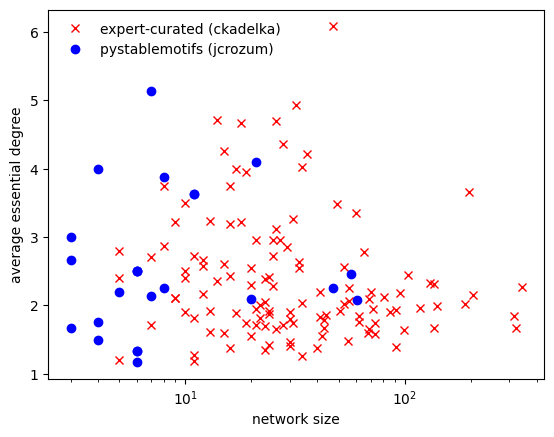
\includegraphics[keepaspectratio]{figures/tutorial11_bio_models_fig0.png}}

\subsection{Null models}\label{null-models}

Observed properties of Boolean networks are often difficult to interpret
in isolation. For example, a network may exhibit a certain number of
attractors, a particular robustness to perturbations, or a specific
Derrida value. However, it is not immediately clear whether such
properties are meaningful or simply typical for networks with the same
size and structural characteristics.

To address this question, researchers compare observed networks with
\emph{null models}: randomly generated Boolean networks that preserve
selected structural features, such as the number of nodes, the wiring
diagram, or the bias of regulatory functions. By analyzing ensembles of
such randomized networks, it becomes possible to determine whether the
behavior of a given network is unusual or expected (see e.g.,
\citet{kadelka2024canalization}).

The BoolForge function
\texttt{random\_null\_model(BooleanNetwork,\ *args)} provides extensive
tools for generating these null models and for performing ensemble-based
analyses that connect structural properties of Boolean functions and
networks with their dynamical behavior.

The function takes as required input a Boolean network. Important: This
network may not contain any degenerate update functions. If it does,
these functions must be simplified via \texttt{bn.simplify\_functions()}
prior to generating null models. The avoid repeating this step many
times, this simplification is not performed inside
\texttt{random\_null\_model}. The type of null model is specified by
optional arguments. Both the wiring diagram and the Boolean update rules
can be randomized subject to specified invariants.

\subsubsection{Randomization of the wiring
diagram}\label{randomization-of-the-wiring-diagram}

By default, the wiring diagram of the provided Boolean network is not
changed. However, setting \texttt{wiring\_diagram="fixed\_indegree"}
generates a new wiring diagram using \texttt{random\_wiring\_diagram}.
Each node in the new wiring diagram has exactly the same in-degree as in
the provided Boolean network.

\begin{lstlisting}
bn_orig = bf.random_network(N=8, n=2, indegree_distribution='Poisson', rng = 3)

bn_null = bf.random_null_model(bn_orig, 
                               wiring_diagram='fixed_indegree')

print('bn_orig.in-degrees:',bn_orig.indegrees)
print('bn_null.in-degrees:',bn_null.indegrees)
print()
print('bn_orig.out-degrees:',bn_orig.outdegrees)
print('bn_null.out-degrees:',bn_null.outdegrees)
\end{lstlisting}

\begin{lstlisting}
bn_orig.in-degrees: [1 2 1 2 1 2 3 2]
bn_null.in-degrees: [1 2 1 2 1 2 3 2]

bn_orig.out-degrees: [4 3 1 0 1 0 1 4]
bn_null.out-degrees: [1 3 1 2 3 2 1 1]
\end{lstlisting}

We see that the in-degrees of the original Boolean network are
preserved, while the out-degrees change substantially. Additional
optional arguments in the \texttt{fixed\_indegree} mode include
\texttt{strongly\_connected}, \texttt{allow\_self\_loops}, and
\texttt{min\_out\_degree\_one}, as described in detail in Tutorial 9.

A more constrained null model fixes the out-degree in addition to the
in-degree. This can be obtained by setting
\texttt{wiring\_diagram="fixed\_in\_and\_outdegree"}.

\begin{lstlisting}
bn_orig = bf.random_network(N=8, n=2, indegree_distribution='Poisson', rng = 3)

bn_null = bf.random_null_model(bn_orig, 
                               wiring_diagram='fixed_in_and_outdegree')

print('bn_orig.in-degrees:',bn_orig.indegrees)
print('bn_null.in-degrees:',bn_null.indegrees)
print()
print('bn_orig.out-degrees:',bn_orig.outdegrees)
print('bn_null.out-degrees:',bn_null.outdegrees)
\end{lstlisting}

\begin{lstlisting}
bn_orig.in-degrees: [1 2 1 2 1 2 3 2]
bn_null.in-degrees: [1 2 1 2 1 2 3 2]

bn_orig.out-degrees: [4 3 1 0 1 0 1 4]
bn_null.out-degrees: [4 3 1 0 1 0 1 4]
\end{lstlisting}

In the \texttt{fixed\_in\_and\_outdegree} mode, the original wiring
diagram is rewired through an edge-swapping algorithm. Additional
optional arguments that can be used in this mode include
\texttt{allow\_new\_self\_loops} and
\texttt{allow\_self\_loop\_rewiring}.

\subsubsection{Randomization of the update
functions}\label{randomization-of-the-update-functions}

In addition to the wiring diagram, the Boolean update functions can also
be randomized. This behavior is controlled by two Boolean flags:

\begin{itemize}
\item
  \texttt{preserve\_bias}: If True (default), the newly generated update
  function of each node has the same Hamming weight (number of ones in
  the truth table) as the original update function.
\item
  \texttt{preserve\_canalizing\_depth}: If True (default), the newly
  generated update function of each node has the same canalizing depth
  as the original update function.
\end{itemize}

If both flags are True (the default), both properties are preserved
simultaneously. If neither flag is True, the newly generated update
rules may be any non-degenerate Boolean function consistent with the
given in-degree.

\begin{lstlisting}

# 8-node network governed by 3-input functions with minimum canalizing depth 1
bn_orig = bf.random_network(N=8, n=3, depth=1, rng = 6)

bn_null00 = bf.random_null_model(bn_orig, 
                                preserve_bias=False, 
                                preserve_canalizing_depth=False)
bn_null01 = bf.random_null_model(bn_orig, 
                                preserve_bias=False, 
                                preserve_canalizing_depth=True)
bn_null10 = bf.random_null_model(bn_orig, 
                                preserve_bias=True, 
                                preserve_canalizing_depth=False)
bn_null11 = bf.random_null_model(bn_orig, 
                                preserve_bias=True, 
                                preserve_canalizing_depth=True)

print('Canalizing depths:')
print('bn_orig:  ',
      [f.get_canalizing_depth() for f in bn_orig.F])
print('bn_null00:',
      [f.get_canalizing_depth() for f in bn_null00.F])
print('bn_null01:',
      [f.get_canalizing_depth() for f in bn_null01.F])
print('bn_null10:',
      [f.get_canalizing_depth() for f in bn_null10.F])
print('bn_null11:',
      [f.get_canalizing_depth() for f in bn_null11.F])
print()
print('Hamming weights:')

print('bn_orig:  ',
      [f.hamming_weight for f in bn_orig.F])
print('bn_null00:',
      [f.hamming_weight for f in bn_null00.F])
print('bn_null01:',
      [f.hamming_weight for f in bn_null01.F])
print('bn_null10:',
      [f.hamming_weight for f in bn_null10.F])
print('bn_null11:',
      [f.hamming_weight for f in bn_null11.F])
\end{lstlisting}

\begin{lstlisting}
Canalizing depths:
bn_orig:   [3, 3, 1, 1, 3, 3, 1, 3]
bn_null00: [0, 1, 0, 0, 0, 0, 0, 0]
bn_null01: [3, 3, 1, 1, 3, 3, 1, 3]
bn_null10: [3, 3, 2, 1, 3, 0, 2, 3]
bn_null11: [3, 3, 1, 1, 3, 3, 1, 3]

Hamming weights:
bn_orig:   [3, 5, 6, 6, 1, 5, 2, 7]
bn_null00: [4, 6, 4, 4, 5, 4, 4, 3]
bn_null01: [5, 5, 6, 6, 3, 3, 6, 1]
bn_null10: [3, 5, 6, 6, 1, 5, 2, 7]
bn_null11: [3, 5, 6, 6, 1, 5, 2, 7]
\end{lstlisting}

We see that the preserved structural constraints determine which
properties of the original network are retained in the null models. Such
controlled randomization allows systematic investigation of how
structural features influence network dynamics.

\subsection{Example use case: high coherence of biological
networks}\label{example-use-case-high-coherence-of-biological-networks}

As an example, we compare the \emph{coherence} of curated biological
Boolean network models with the coherence expected under randomized null
models (see \citet{bavisetty2025attractors}). Coherence measures the
long-term resilience of a network to small perturbations.

For each biological network, we generate an ensemble of randomized null
models in which the wiring diagram is preserved but the Boolean update
rules are replaced by random Boolean functions. We then compare the
coherence of the biological model with the average coherence of its
corresponding null models.

\begin{lstlisting}
n_null_models = 50

bns_to_analyze = [bn for bn in bns if bn.N <= 16]
bio_data = [bn.get_attractors_and_robustness_synchronous_exact()['Coherence']
            for bn in bns_to_analyze]

null_data = []
for bn in bns_to_analyze:
    null_data.append([])
    for _ in range(n_null_models):
        null_model = bf.random_null_model(bn,
                                   preserve_bias=False,
                                   preserve_canalizing_depth=False)
        null_data[-1].append(
            null_model.get_attractors_and_robustness_synchronous_exact()['Coherence']
        )

f,ax = plt.subplots()
ax.plot(bio_data,np.mean(null_data,1),'x')
ax.plot([0,1],[0,1],'r--')
ax.set_aspect('equal', adjustable='box')
ax.set_xlabel('Biological network coherence')
ax.set_ylabel('Average null model coherence')
stat, p = ttest_rel(bio_data,np.mean(null_data,1), alternative='greater')
p_str = f"{p:.2g}" if p >= 1e-3 else "< 0.001"
ax.set_title(f"One-sided paired t-test: p {('= ' if p >= 1e-3 else '')}{p_str}");
\end{lstlisting}

\pandocbounded{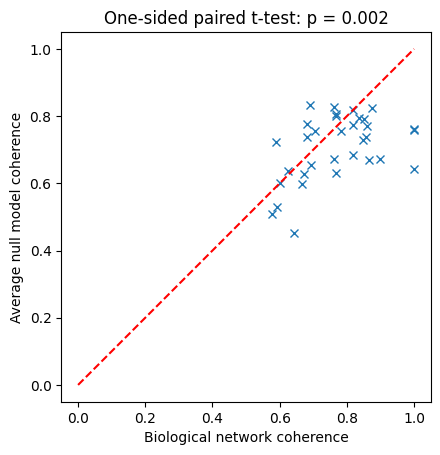
\includegraphics[keepaspectratio]{figures/tutorial11_bio_models_fig1.png}}

We see that most biological networks exhibit higher than expected
coherence. Even for this small ensemble of biological networks
(restricted here to networks with at most 16 nodes to allow exact
dynamical analysis), this is a statistically significant difference, as
exemplified by the one-sided paired t-test.

The higher coherence observed in biological networks is likely due to
their highly biased and canalized regulatory logic (see
\citet{bavisetty2025attractors}). To test this in BoolForge, we can
rerun the computational experiment, this time with null models where
bias and/or canalizing depth are preserved.

\begin{lstlisting}
null_data = []
for i,bn in enumerate(bns_to_analyze):
    null_data.append([])
    for _ in range(n_null_models):
        null_model = bf.random_null_model(bn,
                                   preserve_bias=True,
                                   preserve_canalizing_depth=True)
        null_data[-1].append(
            null_model.get_attractors_and_robustness_synchronous_exact()['Coherence']
        )

f,ax = plt.subplots()
ax.plot(bio_data,np.mean(null_data,1),'x')
ax.plot([0,1],[0,1],'r--')
ax.set_aspect('equal', adjustable='box')
ax.set_xlabel('Biological network coherence')
ax.set_ylabel('Average null model coherence');
stat, p = ttest_rel(bio_data,np.mean(null_data,1), alternative='greater')
p_str = f"{p:.2g}" if p >= 1e-3 else "< 0.001"
ax.set_title(f"One-sided paired t-test: p {('= ' if p >= 1e-3 else '')}{p_str}");
\end{lstlisting}

\pandocbounded{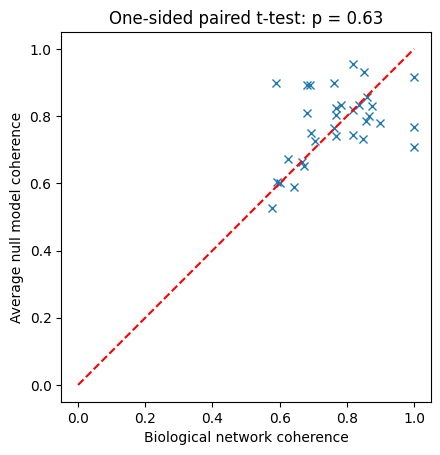
\includegraphics[keepaspectratio]{figures/tutorial11_bio_models_fig2.png}}

We observe that matching canalizing depth and bias (or just one of them,
try it!) suffices to eliminate the significant difference in coherence
between biological networks and their null models.

This illustrates how controlled null models can reveal which structural
properties of biological regulatory logic are responsible for observed
dynamical behavior.

\subsection{Summary}\label{summary-8}

In this tutorial, we introduced \emph{null models for Boolean networks}
and demonstrated how BoolForge can generate randomized networks while
preserving selected structural properties. Such null models provide a
statistical baseline that helps determine whether observed structural or
dynamical properties of a Boolean network are unusual or simply typical
for networks with similar characteristics.

We considered two main classes of null models:

\begin{itemize}
\tightlist
\item
  \emph{Wiring diagram randomization}, where the regulatory graph is
  modified while preserving invariants such as node in-degrees or both
  in- and out-degrees.
\item
  \emph{Update function randomization}, where Boolean update rules are
  replaced by new functions that preserve properties such as bias or
  canalizing depth.
\end{itemize}

In addition, we demonstrated how Boolean network models can be loaded
from biological model repositories and analyzed using the same
structural and dynamical tools provided by BoolForge. This enables
systematic investigation of curated regulatory network models and
comparison with appropriate null models.

Together, these capabilities allow researchers to study how structural
features of regulatory networks influence their dynamical behavior and
to place biological models in the broader context of ensembles of
randomized networks.

\section*{References}\label{references}
\addcontentsline{toc}{section}{References}

\bibliography{references.bib}

\end{document}
